\documentclass[a4paper,12pt]{report}
% Alternative Options:
%	Paper Size: a4paper / a5paper / b5paper / letterpaper / legalpaper / executivepaper
% Duplex: oneside / twoside
% Base Font Size: 10pt / 11pt / 12pt

\usepackage{hyperref}
\hypersetup{
    colorlinks,
    citecolor=blue,
    filecolor=black,
    linkcolor=blue,
    urlcolor=blue,
    bookmarksopen = false,
    pdfstartview = {XYZ null null 1.00}
 	%pdfpagemode=None
}
\usepackage{enumerate}

%for showing sub sub section number and table of content upto level 3
\setcounter{secnumdepth}{3}
\setcounter{tocdepth}{3}
%for landscape image
\usepackage{lscape}


\hypersetup{linktocpage}

%% Language %%%%%%%%%%%%%%%%%%%%%%%%%%%%%%%%%%%%%%%%%%%%%%%%%
\usepackage[USenglish]{babel} %francais, polish, spanish, ...
\usepackage[T1]{fontenc}
\usepackage[ansinew]{inputenc}
\usepackage{amsmath}
\usepackage{lmodern} %Type1-font for non-english texts and characters
%\usepackage{hyperref}
%\usepackage[hypertex,backref=false,bookmarks=true]{hyperref}
%% Packages for Graphics & Figures %%%%%%%%%%%%%%%%%%%%%%%%%%
\usepackage{graphicx} %%For loading graphic files
%\usepackage{subfig} %%Subfigures inside a figure
%\usepackage{tikz} %%Generate vector graphics from within LaTeX
\usepackage{caption}
\usepackage{subcaption}
%% Please note:
%% Images can be included using \includegraphics{filename}
%% resp. using the dialog in the Insert menu.
%% 
%% The mode "LaTeX => PDF" allows the following formats:
%%   .jpg  .png  .pdf  .mps
%% 
%% The modes "LaTeX => DVI", "LaTeX => PS" und "LaTeX => PS => PDF"
%% allow the following formats:
%%   .eps  .ps  .bmp  .pict  .pntg


%% Math Packages %%%%%%%%%%%%%%%%%%%%%%%%%%%%%%%%%%%%%%%%%%%%
%\usepackage{amsmath}
%\usepackage{amsthm}
%\usepackage{amsfonts}

%\usepackage[pdftex]{graphicx}
%% Line Spacing %%%%%%%%%%%%%%%%%%%%%%%%%%%%%%%%%%%%%%%%%%%%%
%\usepackage{setspace}
%\singlespacing        %% 1-spacing (default)
%\onehalfspacing       %% 1,5-spacing
%\doublespacing        %% 2-spacing


%% Other Packages %%%%%%%%%%%%%%%%%%%%%%%%%%%%%%%%%%%%%%%%%%%
%\usepackage{a4wide} %%Smaller margins = more text per page.
%\usepackage{fancyhdr} %%Fancy headings
%\usepackage{longtable} %%For tables, that exceed one page

%%%%%%%%%%%%%%%%%%%%%%%%%%%%%%%%%%%%%%%%%%%%%%%%%%%%%%%%%%%%%
%% Remarks
%%%%%%%%%%%%%%%%%%%%%%%%%%%%%%%%%%%%%%%%%%%%%%%%%%%%%%%%%%%%%
%

\usepackage[titletoc]{appendix} % use the appendices environment for Appendix
\usepackage[numbers]{natbib}
%\setcitestyle{numbers}
%\citestyle{plainnat}
\usepackage{tabularx}
\usepackage{cleveref}
\crefname{subsection}{subsection}{subsections}
%\usepackage{pdfpages}
%%%%%%%%%%%%%%%%%%%%%%%%%%%%%%%%%%%%%%%%%%%%%%%%%%%%%%%%%%%%%
%% DOCUMENT
%%%%%%%%%%%%%%%%%%%%%%%%%%%%%%%%%%%%%%%%%%%%%%%%%%%%%%%%%%%%%
\begin{document}

%Title
\begin{titlepage}
\pagestyle{plain}

\thispagestyle{empty}
\begin{center}

 \LARGE UNIVERSIT\`A DEGLI STUDI DI TRENTO\\

\textbf{\large Facolt\`a di Scienze Matematiche, Fisiche e Naturali
   }\\

\begin{figure}[h!]
 \centerline{
\includegraphics[width=0.7\textwidth,height=2in]{Logo/ulogo}}
\end{figure}
%\normalsize
%\vspace{0.1 cm}
\begin{center}
Corso di Laurea Magistrale in Informatica
\end{center}
\hrulefill
\begin{center}
Final Thesis
\end{center}
\end{center}
\vspace{0.3 cm} %\LARGE\textsc{Adaptive Human-Computer Interaction For An Interactive Mobile Application\\Case Study : Smart Cafeteria\\}
\begin{center}
 \LARGE \textsc{\textbf{``Smart Cafeteria'' Adaptive And Interactive Mobile Application} \\}
\end{center}
\vspace{2cm}

\begin{minipage}{0.5\textwidth}
\begin{flushleft} 
\large
\emph{Supervisor:} \\
\textbf{Antonella De Angeli}\\
Associate Professor(DISI)\\
University of Trento(Italy).
\end{flushleft}
\end{minipage}
\begin{minipage}{0.5\textwidth}
\begin{flushright} 
\large
\emph{Author:}\\
\textbf{Supta Richard Philip}\\
\small supta.philip@gmail.com
\end{flushright}
\end{minipage}

\vspace{1.4cm}
\begin{center}
%\normalsize
July $2013$
\end{center}
\end{titlepage}

\newpage
\thispagestyle{empty}
\mbox{}
%Abstract
\begin{abstract}
\phantomsection
\addcontentsline{toc}{chapter}{Abstract}
\thispagestyle{plain}
\pagenumbering{roman}
\setcounter{page}{1}
% \noindent
Mobile Human-Computer Interaction is the relationship (interaction) between
people and their handheld mobile systems and the applications which we use in
our everyday life. In a word, mobile applications are interactive products to
support users in their day to day life no matter where they are. Since
technology is moving fast and changing rapidly, it is very important to
understand the mobile interaction techniques and the impact of possible mobile
technologies on human life. Mobile HCI concerns about the mobile applications
and PDA which discusses the different possible interaction techniques with those
applications. In the university cafeteria provides services manually to the
students which cause different kinds of problems such as losing time in
cafeteria queue, unable to browse and choose meal in advance, does not provides
any kind of dieting advices to students which help them to keep proper dieting.
In this thesis, I have proposed an adaptive, interactive mobile application
which is called ``Smart Cafeteria'' that will provide services to the university
students and faculties for managing their meal in the universities' cafeterias
which in consequence makes their life more easy and comfortable. In this work
from beginning to end, I have followed HCI interaction design methodology in
every step such as problem define, data gathering, requirement analysis,
prototype development and usability evaluation for ``Smart Cafeteria''
application.\\ \\
\textbf{Keywords:} Mobile Human-Computer Interaction, Adaptive HCI, Interactive
Mobile Application, Smart Cafeteria.
\end{abstract}
\newpage

\newpage
%\thispagestyle{empty}
\mbox{}
%Acknowledgement
\setcounter{page}{2}
\phantomsection
\addcontentsline{toc}{chapter}{Acknowledgement}
\chapter*{Acknowledgement}
First of all, I would like thank Almighty God for His kindness.

Then I would like to thank my honorable adviser Professor Antonella De Angeli
who give me the opportunity to work with her and to carry out this thesis work.
During my work, her guidance and advice, especially in the time of my research
helped me come across a long way to accomplish this thesis work. Unless her
supports, inspirations, and encouragements it would have been impossible to finish
this thesis.

I would like to thank Silvia Torsi for providing ideas and some materials
related to this  work.

I am grateful to my beloved Tithi Florence D'Costa to encourage me all the time
to complete this work.

My heartiest gratitude to all Bangladeshi Students in Trento, especially Ashish
Kumer Basak, Miah Raihan Mahmud Arman, Kazi Asad Robin, Abarat Hossain, Tohedul
Islam to support me all the time and unless their help, it would have been
impossible to complete this work.

\newpage

\newpage
%\thispagestyle{empty}
\mbox{}
%Dedication
\phantomsection
\addcontentsline{toc}{chapter}{Dedication}
\chapter*{Dedication}%

This work is dedicated to my Family Members who are been long waiting for my
return back to home with success.
\newpage

\newpage
%\thispagestyle{empty}
\mbox{}
%Table of Content
\phantomsection
\addcontentsline{toc}{chapter}{Table of Contents}
\renewcommand{\contentsname}{Table of Contents}
\tableofcontents 

\clearpage
\newpage
%\thispagestyle{empty}
\mbox{}
%List of Fiqure
\cleardoublepage
\phantomsection
\addcontentsline{toc}{chapter}{\listfigurename}
\listoffigures

%List of Table
\cleardoublepage
\phantomsection
\addcontentsline{toc}{chapter}{\listtablename}
\listoftables

\newpage
%\thispagestyle{empty}
\mbox{}

\newpage
\setcounter{page}{1}
\pagenumbering{arabic}


\chapter{Introduction}
\label{chap:Introduction}
One of the most common and fundamental necessity of life is food. It is not only
about the joy of eating, it also has an intimate relationship with the important
factors of human life such as health, dietary, entertainment. Many people who
are busy in their work place, have to take their breakfast and lunch at
cafeteria or Restaurant. In that case, time, quality of food and appropriate
food are very important fact. Those people needs some extra facilities for
planning their menu and save their time for searching food and also spend less
time in the queue for food. It is obvious that, good and enjoyable food in a
short time would improve the quality of life\footnote{Some ideas \& contents
have taken from Silvia Torsi, Researcher, University of Trento.}.

``Smart Cafeteria'' is a part of Smart Campus project\footnote{This work is a
part of \href{http://www.smartcampuslab.it/}{Smart Campus} project funded by
\href{http://www.trentorise.eu/}{Trento RISE}.} funded by Trento RISE. The goal
of the project is to provide advanced Information and Communication Technology
(ICT) solutions to all people  involved in a University campus; namely to
provide innovative services to support their lives.

\section{Problem Statement}

In this section, I will discuss two real life scenarios which happens quite
often students and professors.

\subsection{Scenario 1: Hungry Student}
\label{HungryStudent}
XXX is a second year student, he has a lot of friend, he spends most of his day
at the University. His classes usually ends at 13.00 then he always have to
wait for his friends. Eventually when he reaches the canteen to eat with his
friends, he always finds long queue of students waiting to take food.
Furthermore he would prefer to know the menu of the canteen before standing in
the queue but he has to wait because of the huge gathering of students in queue.
Even when he reaches the food counter it takes a long time to prepare the food
he ordered. He is also not happy with the decreasing quality of the food in the
canteen. He also finds the canteen a  boring place to sit and chat with friends
as there is always huge gathering of students during the lunch break.

\subsection{Scenario 2: Busy Professor}
\label{BusyProfessor}
Mr. YYY is a professor of Computer Science who is busy with a lot of things like
research work, teaching in class, presentation talk, meetings. He does not have
enough time to choose food standing in the queue of the canteen. So he is
thinking if there will be a system where user can choose and order their lunch
even before going to the canteen, it would be even better if the system can
suggest dietary as well. If he can access the system through his mobile phone
from anywhere around the university it would make him a really happy professor.
\subsection{Real Life Problem}
In the previous section [\ref{HungryStudent},\ref{BusyProfessor}], I have
discussed two real life scenarios where technological service will make our life
more easy. Providing good facilities for eating can be a simple way to improve
campus life by the university cafeteria. Standing in long queues in cafeteria
for food takes out a good amount of time from student's and staff's
daily working routine. Additionally waiting in the queue without knowing the
menu for a particular day can be time killing if someone finds nothing
satisfactory to eat. The facility of knowing the menus in advance is a recurring
request. The canteen is a space for students to pass some quality time eating
and discussing with their friends similar for that university staff's with their
colleague's.

Daily and weekly menu are not available at cafeteria in advance and there is no
way to know cafeteria is open or not before going to the cafeteria physically.
It is always important to maintain proper diet from dieting suggestions
to keep healthy life. Healthy and happy life always has a great impact on daily
works such as study, research, job.

In this research, I have tried to figure out the possible answeres and solutions
of following questions:
\textbf{
\begin{enumerate}[(I)]
  \item How to skip the long queue of cafeteria such that no waiting more than 5 minutes to
  take food.
  \item How to know the menu of the cafeteria before standing in the queue;
  namely from any another places.
  \item How technology can help us in selecting meal from cafeteria more comfortably.
  \item How to know the most appropriate menu for me in terms of calorie contains and price.
  \item How to collaborate and share my feeling with others when I am in cafeteria.
\end{enumerate}
}


\section{Objectives}
In this thesis work, I have applied user centered design methodology and found
some possible services of Smart Cafeteria. First of all, I have applied
PACT\footnote{\href{http://hci.ilikecake.ie/requirements/pact.htm}{PACT
Analysis}} analysis on Smart cafeteria and figured out the following factors
through this analysis.

\textit{\textbf{Places:}} Meeting places for students, researchers and professors; the
canteen, the queue.

\textit{\textbf{Activities:}} Finding food menu to eat, avoid queue, choosing
the meals, eating, choose diet menu.

\textit{\textbf{Context:}} The university life, The activity of eating.

\textit{\textbf{Technologies:}} Web 2.0, SmartPhone.

Finally there are some services which should be considered in case of smart
cafeteria. In the thesis work, I will try to emphasize and develop such an
interactive, adaptive system to provide the following services:
% \begin{itemize}

\begin{enumerate}
%\addtocounter{enumi}{-1}
\item  \textit{\textbf{Mensa Queue Skipper:}} A system of booking food menu from
the canteen that makes the students wait no more than 5 minutes.
Queues in the canteen and at the administration services results loosing time.
Students often feel that the University cafeteria system is not enough to
provide them good supports for their daily lunch activities. This is due to
large number of students with respect to the number of personnel's providing
services in cafeteria. Technology could easily help them avoid queue. If all
member of the university could be able to access everydays food menu as a list
or search for their preferable menu with the help of an application as well as
ordering food and paying for the food through the application, It could be a
solution to skip queue in the cafeteria.

\item \textit{\textbf{Menu Finder:}} Daily and weekly menus of the University of
Trento cafeteria' are available on the website which is offered by cafeteria's
stuff in a specific format. But most of university's members do not notice that
information and the system does not notify them. So it is obvious that
university's cafeteria must need a menu finder to help them to search their
appropriate food menu which is offered by the cafeteria.

\item \textit{\textbf{Menu Suggester and Dieting Adviser:}} Students' dieting is
a very important issue that should not be left to chance. Some research
\cite{HealthyDiet} shows that the students' recurrent lack of information about
dieting, proper food combining meal plans, balance dieting and this could be an
obstacle to improve their general health and well being. So indications of
dieting measures in a cafeteria system such as Menu Suggester and Dieting
adviser depend on users' choice and how much calories they consumed in the last
couple of weeks could be a very good solution for Smart Cafeteria.

\item \textit{\textbf{Create Customized Menu:}} People can order food and make their
own menu in the restaurant according to their own choice and as much as food
they need. In the system application point of view, giving the user freedom to
create their own menu from different food could be a very smart thinking.

\item \textit{\textbf{Lunch with Friend:}} Create a collaborative application
where user can follow their friends; can see the activities of friends and share
the activity of meals. This may give newcomers and foreign students the
possibility to exchange language or psychological peer supporting.

\end{enumerate}

%\end{itemize}

The goal of the thesis is to develop just in time service where students,
professors, rersearchers do not need to wait too long to order food, we will
imposed such a system where students and staffs will be able to order their food
online even before going to the cafeteria physically. Daily and weekly menu will
be made available in the system which will also give suggestions of dieting
measures. The system will also suggest food according for their choice and the
calorie requirement. So the main objectives of this thesis are to:
\textbf{
\begin{enumerate}[(I)]
\item Create ``Smart Cafeteria'' which will be supported by web 2.0 system and
Smartphone application.
\item The application should be adaptive and interactive.
\end{enumerate}
}
There is also couple of sub goals which overlap with the main objectives of this
thesis. The sub goals are:
\textbf{ \begin{enumerate}[(i)] 
\item Provide online cafeteria services.
\item Provide dieting services to the students.
\item  Provide social collaboration services in the application.
\end{enumerate}
}

\section{Structure of Thesis}
The thesis is organized as follows:

% Chapter~\ref{chap:Introduction}, \textit{Introduction}, describes the set of
% scenarios, defines the problem statement and state the contribution of this
% work. This chapter also includes the organization of the thesis reflexively.

Chapter~\ref{chap:StateofArt}, \textit{State of Art}, highlights Human Computer
Interaction (HCI), its goals and adaptive HCI. It is also described Interaction
Design and its Process, Goals, Principles and Usability Heuristics. In the last
two sections of this chapter are discussed Interactive Mobile HCI and Benchmark
Analysis using some related mobile applications.

Chapter~\ref{chap:AnalysisofSmartCafeteria}, \textit{Analysis of Smart
Cafeteria}, discusses Requirements and Data Gathering techniques and processes
of ``Smart Cafeteria'' which help to find Stakeholders, initial Functional
Requirements and Non Functional Requirements as well as stable requirement using
Studying Document, Focus Group and Questionnaires. Finally Data Analysis has
been done using UML 2.0 such as use cases, class diagram and activity diagrams.

Chapter~\ref{chap:DesignofSmartCafeteria}, \textit{Smart Cafeteria Design},
presents Conceptual Architecture and Design, Mid-fadelity UI for both desktop
and Mobile version of Smart Cafeteria; and finally discusses Key Features of
the application as a mobile application.

Chapter~\ref{chap:EvaluationSC}, \textit{Usability Evaluation of Smart
Cafeteria}, reports Evaluation Methodology and Evaluation Result such as user
observation and Questionnaire for usability evaluation for both desktop and
mobile prototype. Finally Suggestions for Improvement has been presented.

Chapter~\ref{chap:Conclusion}, \textit{Conclusion}, concludes the overall
achievements of the thesis work and possible extensions of the work are being
presented.



\newpage
%\thispagestyle{empty}
\mbox{}

\chapter{State of Art}
\label{chap:StateofArt}
In this chapter, first section [\ref{sec:HCI}] is dedicated for discussion
related to HCI, its goal and adaptive HCI. In the second section [\ref{sec:ID}],
I have discussed interaction design, its processes, goals, principles and
usability heuristics. In the following sections [\ref{sec:IMA}, \ref{sec:RMA}],
I have discussed interactive mobile application and some related mobile
applications from google play store, which offers some similar feature as like
our proposed ``Smart Cafeteria'' application respectively.

\section{Human Computer Interaction}
\label{sec:HCI}
Human Computer Interaction is a area of research and study which deal with
analysis, design of interactive application by involving its users in
the design process; and focuses on the interaction between Human and computer
application. In some cases, HCI is also known as man-machine interaction (MMI) or
computer-human interaction (CHI). In recent years, there was a great progress in
the field of Mobile human interaction which invloves interaction between users
and mobile applications.

According to \citet{Love:2005:UMH:1076935},  HCI is concerned with looking into
the relationship between human and computer systems and applications that people
use on their everyday life. Since HCI or Mobile Human Interaction is concerned
with investigating the relationship between people and systems or applications,
we are always concerned with understanding the users as well as their various
capabilities and expectations and how these can be taken place into the mobile
system or application design. In the any HCI design process or Interactive
mobile system design, User should be emphasized first and then the other key
aspects are firstly what tasks users want to perform when using the system;
secondly which characteristics of the user could have a significant effect on
their performance with the system; thirdly developing  the system which meet the
users needs and finally the evaluation of the developed system should check if
it meets users' needs as well as satisfying to use and getting users' feedback
which helps to develop updated version of the system. So this includes the
factors such as an understanding of the user and their task what they want to
perform in the system,  the design tools and software packages that are needed
to achieve usability of the system.

\citet{Yang2009} state that the ultimate goal of Human-Computer Interaction
research is exploring how to design the computer or system application to help
people to complete the necessary tasks more safely and efficiently. However the
computer is still a tool and in that case, people and the computer communicate
with each other through the system interface consisting hardware and software. To
achieve that communication effectively and efficiently is called interactive
system design methodology. The main thing is that are those communication really
efficient and effective or enjoyable during usage? All these questions
and answers we will figure out in HCI research work.


\subsection{HCI Goals}
The basic goal of Human-Computer Interaction is to improve interaction between
users and computer  by making applications and computers more usable and
receptive to the user's needs. That means that we want to make the system easy,
safe, effective and enjoyable and to decrease  barrier as much as possible
between human's cognitive model and  user tasks \cite{Sandrahci}. The principle
aim of Human Computer Interaction is to design interactive and safe functional
software system with good usability.

Basically Human Computer Interaction concerns about:
\begin{itemize}
\item \textbf{Process of design interfaces, prototypes and their methodologies:}
HCI concerns about designing the best possible interface, prototype and
development considering user needs and  optimizing the design to achieve desired
functionality in term of learnability ,efficiency of use, effectiveness of use,
enjoyable to use.
\item \textbf{Methods for implementing interfaces and prototype:} HCI also
concerns about methods of software developments, software toolkits and
libraries, efficient algorithms for developing inferface, prototypes and
implementing in real products.
\item \textbf{Methods of evaluating and comparing interfaces and prototypes:}
This is one of the most important part in HCI and interactive product design
which involves user interview, review of application that ensure usability of
application.
\item \textbf{Developing new interfaces, prototypes and interaction techniques:}
This part involves in re-design and evaluating the design of the application.
\end{itemize}

\subsection{Adaptive HCI}
Even the most sophisticated machines will be worthless if user cannot use them.
With time HCI has travelled a long way forward from the start of the concept.
Intelligent and Adaptive HCI is a part of HCI with the goal of research to
improve HCI by using smarter and newer technology. HCI has been influenced a lot
by all the researches of AI technology as AI addresses to topics important for
HCI like adaptability and problem solving.

The main aim of the Intelligent HCI is to enhance the flexibility, usability and
the human-computer interaction. This interaction between men and machine is not
limited to computers only but also with all other machine used in our day to day
life like, television, refrigerator, mobile phones, cars. Nowadays most of the
Intelligent HCIs have the ability to learn from the environment and work
accordingly to reach its goal. Intelligent technologies are used to achieve the
intelligent and adaptive HCI but the goal always remains the same which is to
improve the communication between users and machines. Several techniques are
used to achieve this goal like intelligent input technology, user modeling, user
adaptivity, explanation generation.


An adaptive HCI might be a website using regular GUI for selling various
products. This website would be adaptive -to some extent- if it has the ability
to recognize the user and remembers his searches and purchases and intelligently
search, find, and suggest products on sale that it thinks user might need. Most
of these kind of adaptation are the ones that deal with cognitive and affective
levels of user activity \cite{karray2008human}.

\citet{Lo2006} discussed in his paper that identifying the user's
characteristics is the key for developing adaptive Web-based systems. He also
proposed an adaptive architecture
[Figure-~\ref{AdaptiveApplicationArchitecture}] according to that architecture, 
adaptation decision in an adaptive web-based system depends on user
characteristics which is represented in the user model. An adaptive Web-based
system is helpful to deliver information to users more efficiently and
effectively.
\begin{figure}[h!t]
    \centering
        \fbox{
      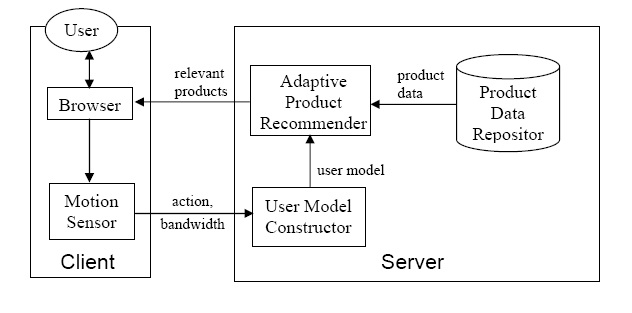
\includegraphics[width=5.5in]{ch2/AdaptiveApplicationArchitecture/adaptive_application_architecture}
      }
  \caption{Adaptive Application Architecture}
  \label{AdaptiveApplicationArchitecture}
\end{figure}

According to his architecture, there are three components in the server: Product
Data Repository, User Model Constructor, and Adaptive Product Recommender. The
Product Data Repository stores the product into database. The User Model
Constructor, together with the observed user browsing behavior, are responsible
for building and updating the temporary user model for incremental learning of
the user's interests. The Adaptive Product Recommender is responsible for
determining the recommendation sequence and the presentation of products in the
user interface based on Product Data Repository and the user model.

\section{Interaction Design}
\label{sec:ID}
A main goal of interaction design is to develop interactive software products
that are usable which means the software should be easy to learn, effective to
use, and should provide an enjoyable experience from the user's perspective
\cite{preece2002interaction}. Designing usable interactive products
requires consideration of the users of software product and the context; means who is
going to use the product and where they are going to be used. Another important
aspect is understands the type of activities performed by users when they
try to interact with the products. The perfectness of different kind of
interfaces and arrangements of input and output factors depends on different type of
activities need to be supported. The aim of interaction design is to provide
redress this concern by bringing usability into the design process. Through
interaction design process, we design interactive products to support people in
their everyday  lives. The main key view of Interactive design is easy,
effortless, and enjoyable.

Interactive system design being a part of Human Computer Interaction is a
multidisciplinary area where various subjects and disciplines such as
Psychology, Computer Science, Sociology, Design contribute its knowledge and
research works supporting on both the machine and the human factors such as
computer user satisfaction. Interactive system design involves several
disciplines and some of them are shown in Figure~\ref{DisciplinesInvolvedID}.
\begin{figure}[h!t]
    \centering
      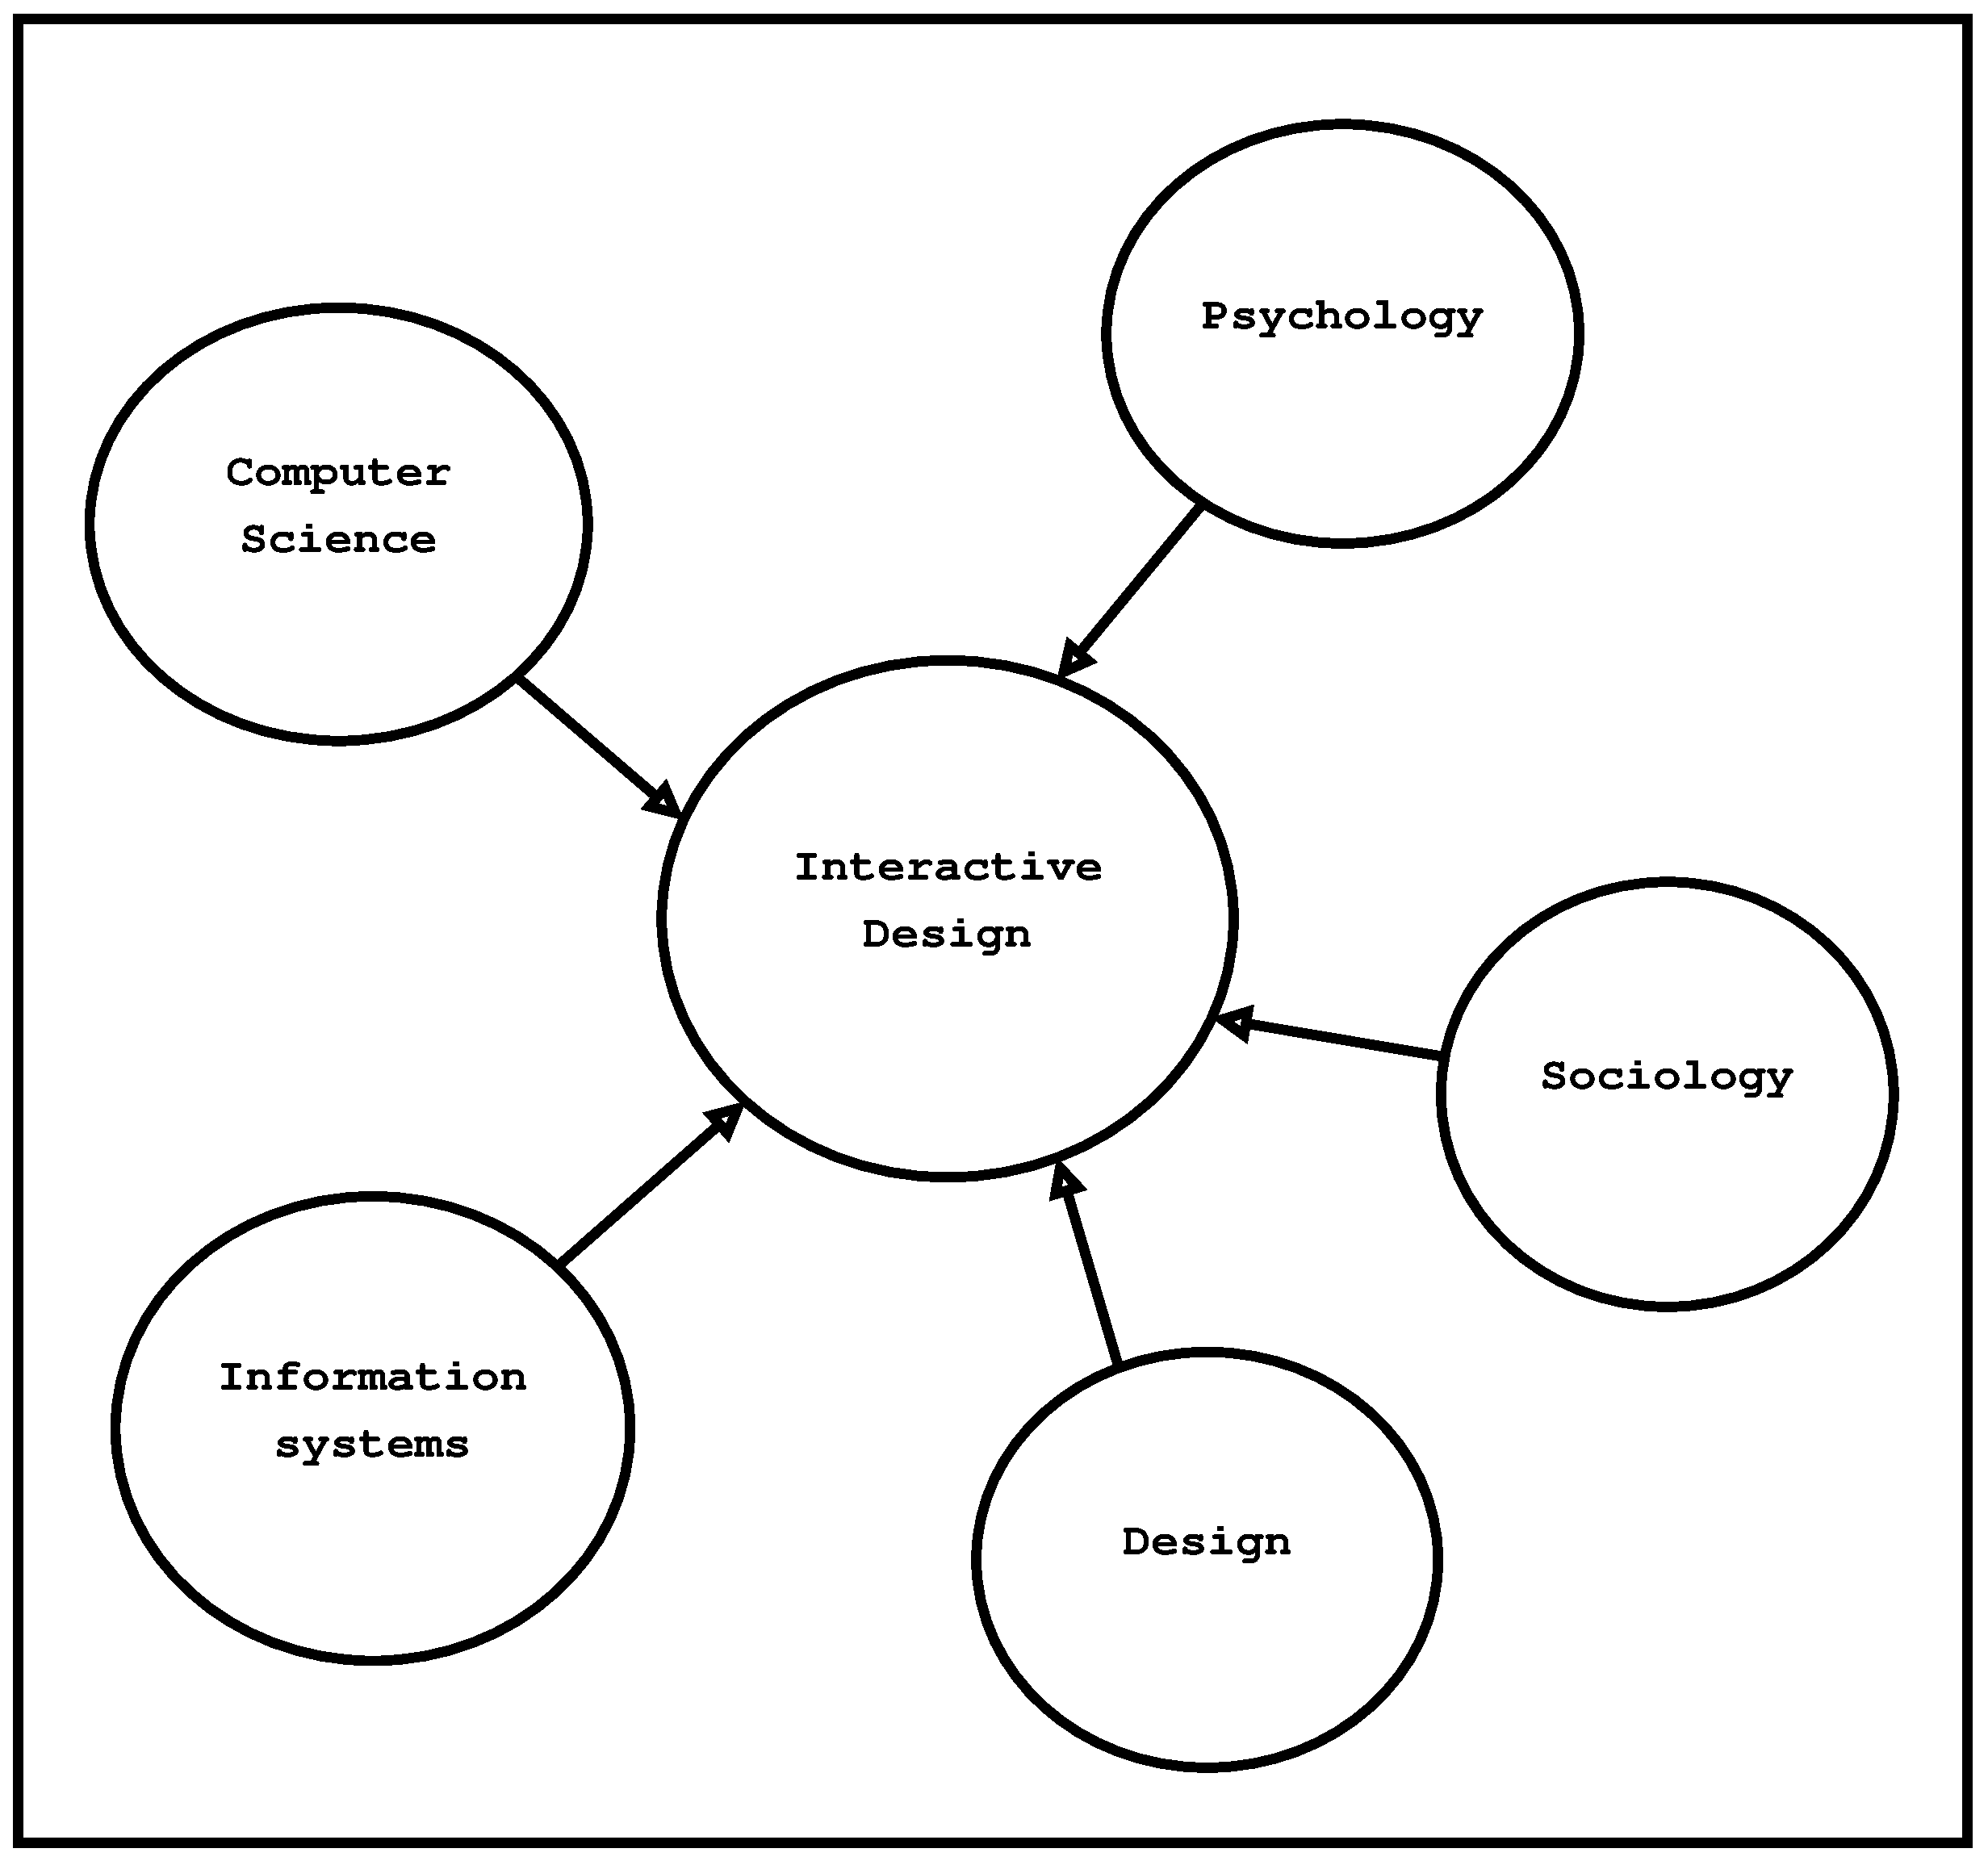
\includegraphics[width=5.5in,height=4in]{ch2/DisciplinesInvolvedID}
  \caption{Disciplines involved in Interactive system design [adapted from \cite{Love:2005:UMH:1076935,preece2002interaction}]}
  \label{DisciplinesInvolvedID}
\end{figure}


\subsection{Interactive Design Process}
According to \citet{Yang2009}, there has not any unique
standard for interactive design in theory, and there's still mainly concept and
model from the software industry. In the field of product design, many new
subjects and situations could happen and the industrial designers need to keep
in practice and study to use the old theory of interaction design principles and
should do more research to sum up  interactive principle and theory which can
suit for target product design and planning. There are three key characteristics
of the interaction design process \cite{preece2002interaction} which should be kept
in mind when we are going to develop any interactive product:
\begin{itemize}
\item Users need to be involved in the development  process.
\item  Specify usability and user experience goals, identify them clearly and
document them properly  at the beginning of the project.
\item  Iteration through the basic four interaction design activities.
\end{itemize}

Fundamentally, the process of interaction design \cite{preece2002interaction} involves four basic
activities:
\begin{enumerate}
\item \textbf{Identifying needs and establishing requirements:} In order to
design some interactive system, we must know about target users and what kind of
services an interactive product could usefully provide.
We should always find out goals and needs of product from the point of view
users. And finally establish a set of requirements which will help to design and
develop product.
\item \textbf{Developing alternative designs that meet those requirements:} This
is the core activity of designing an interactive product which basically suggesting
ideas to meet the requirements. This could  be divided into two sub parts:
conceptual design that means  developing a conceptual model of the product which
describes what the product should do, behave and seems like; and physical design
considers the detail of the product including the colors, sounds, and images of
the product template namely  menu design, icon and interface design.
\item \textbf{Building interactive versions of the designs:} There are sensible
ways for users to evaluate interactive versions of the designs which should be
built, but that does not mean that the final version of the software is required.
There are several techniques to achieve interactive version of product; namely
prototyping, but it does not require a complete software. There are different
prototyping techniques; among them paper-based prototypes are very quick and
cheap for building demo and those are very effective for identifying problems at
the very beginning stages of software design, and through  that  users can get a
real sense of  the product to interact with.
\item \textbf{Evaluating the designs:} Evaluation is the way to determine the
usability and acceptability of product design, which means it is measured
variety of criteria namely the number of errors user make when they are using
it, how attracting it is, how well it matches the requirements, and so on.
Interaction design need  user involvement throughout the development and this
increases quality of the product and confirm final product's quality.
\end{enumerate}
These four steps in interaction design model contains iteration and involves
user in evaluation. From these steps, perhaps some alternative designs could be
generated in some attempts that meet the needs and requirements of the
application. Then interactive design versions of application are developed and
evaluated iteratively. Based on the feedback of the evaluations namely
interviews, users group;  it could return to the step for identifying needs or
refining the previous requirements. In the figure \ref{fig:SimpleLifeCycleID} a
simple lifecycle model of interaction design has been shown\footnote{This image
is adapted from Interaction design: beyond human-computer interaction.}.
\begin{figure}[h!t]
    \centering
      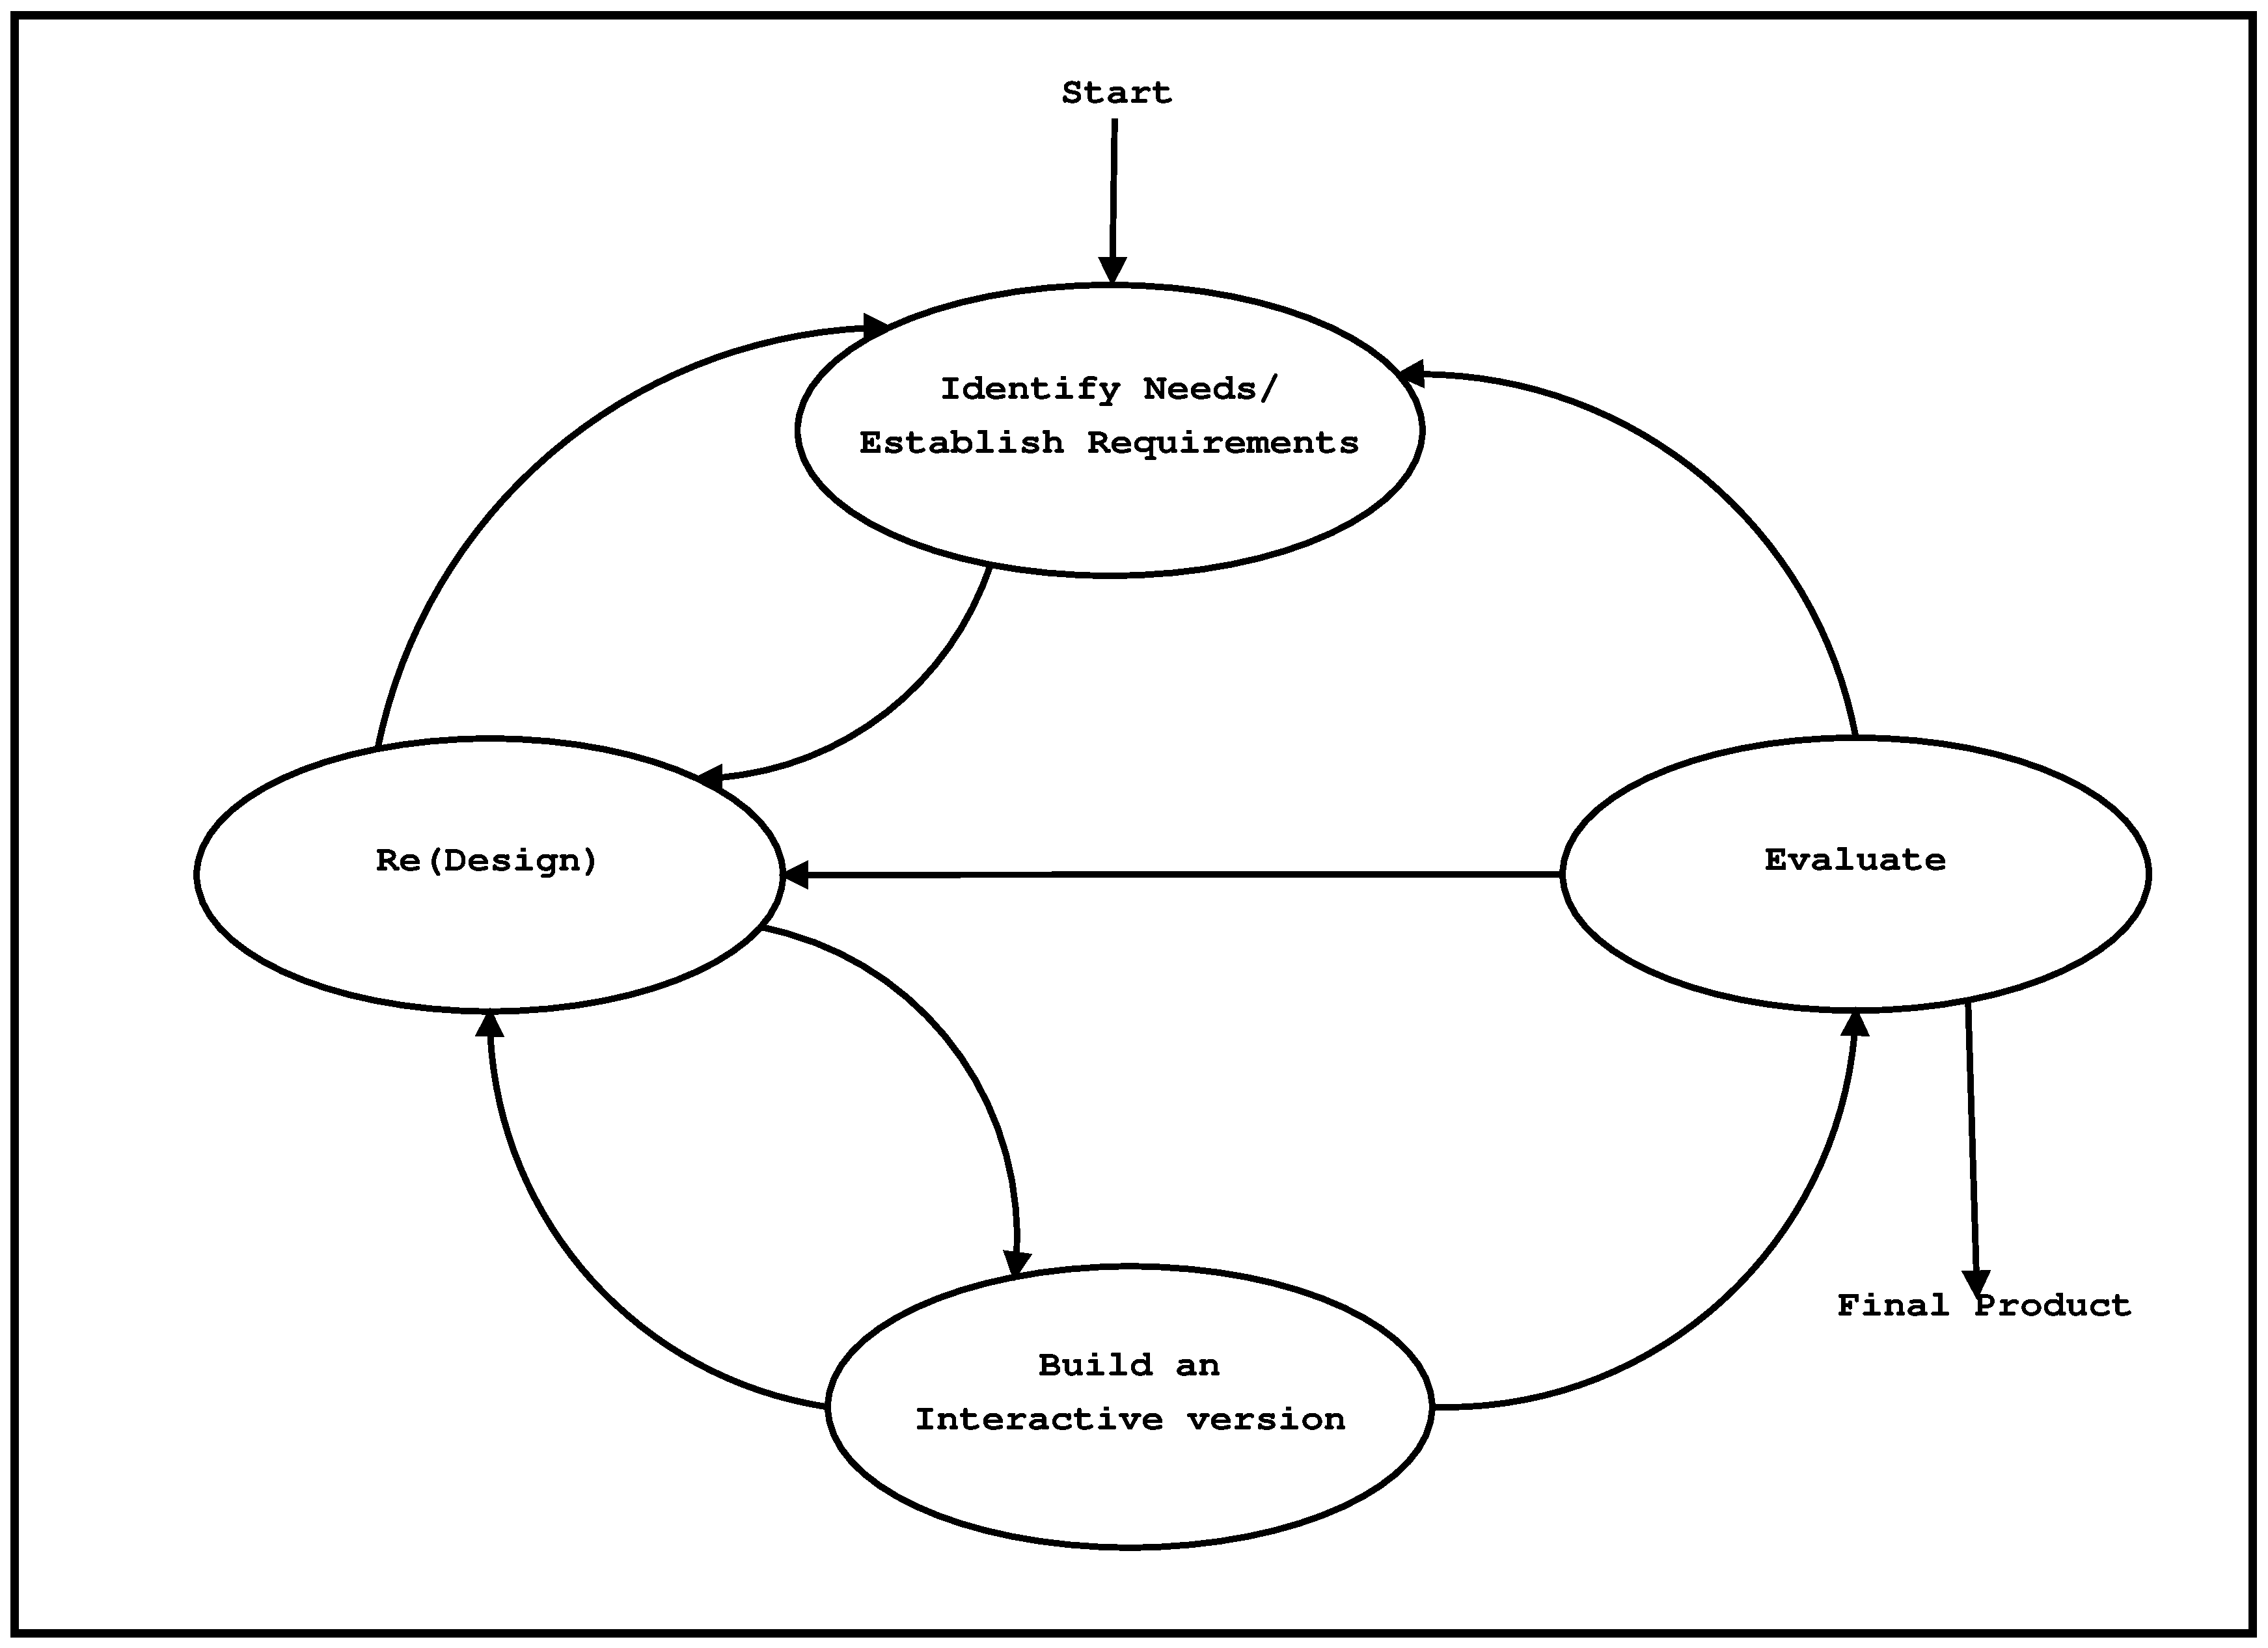
\includegraphics[width=5.5in,height=4in]{ch2/SimpleLifeCycleID}
  \caption{A Simple Life Cycle of Interaction Design Process.}
  \label{fig:SimpleLifeCycleID}
\end{figure}

\subsection{Goals and Principles}
The goals of interactive software design mainly concentrates on usability goals
which ensure that developed applications are easy to learn, efficient to use,
safe to use, effective to use, easy to remember and enjoyable from users'
perspective \cite{preece2002interaction}.
Optimizing alternative connection of people and products are the main objective
of interactive product design. It requires the designers to consider the great
anticipations of the users. Satisfying users' expectation and extending them
to potential needs. Here are the basic principles \cite{Yang2009} of Interactive
product design:

\begin{enumerate}
\item \textbf{Visibility:} In the implementation of application's controls and
functions should follow user perception of the application's operation and the
user's mental model of that application as much as possible. To be compatible
with psychological needs of the users, functions of the product should be
developed in a way so that users can understand and control it properly.

\item  \textbf{Correct and clear feedback:} Somehow  correct and clear feedback
is related with Visibility. Application receives command from different
functions, for execution it should follow a variety of sensory feedback in the
right manner to make access and control of the  system pleasurable, efficient
and canonical.

\item  \textbf{Constraints:} It can be put to practice through physical, logical
and common sense of cultural aspects of interactive product design. Users must
take the correct actions of cross-function to control the enter into the system
forcefully to avoid human errors. To enhance the interaction easy to learn, the
design can be created with safe and reliable use of the environment.

\item  \textbf{Mapping and Matching:} Control of information and
feedback should be able to establish a direct relationship efficiently and
accurately. This is the assurance of user's interactive behavior.

\item \textbf{Consistency:} The psychological vulnerability and memory of user
has a direct impact on the efficiency of the control of the application.  All
the above principles should be followed by the designers in successful
interactive system designs. The designers have to take the psychological feeling
into account and should make the product in a way so that it have a positive
effect in the day-to-day use when they executes the functions.

\end{enumerate}

\subsection{Usability Heuristics}
\label{sec:HeuristicsUsability}
Interactive Design principles incline to be used mainly for developing a new
design, whereas usability principles known as Usability Heuristics are used
mostly as the basis for evaluating prototypes and existing applications. Below
ten usability principles are described which were developed by Nielsen
\cite{Nielsen1990}. Observe that some of them overlap with the interactive
design principles.

\begin{enumerate}
\item \textbf{Visibility of system status:} The system should always inform
users about what is going on in the system and should also provide appropriate
feedback within reasonable time.
\item \textbf{Match between system and the real world:} The system should
provide services using the users' language, rather than system oriented terms
and should follow real world conventions, making information appear in a natural
and logical order.
\item \textbf{User control and freedom:} The system should provide the ways such
as control and freedom to users; if somehow they are stuck somewhere within
system, they could easily escape from that unexpected situation themselves 
using clearly marked emergency exits.
\item \textbf{Consistency and standards:} The system should avoid making users
wonder where different words, actions and situations  mean the same thing and
should follow standard  conventions.
\item \textbf{Help users recognize, diagnose, and recover from errors:} The
system should use plain and easy  language to describe the nature of the problem
and suggest a way to solve it.
\item \textbf{Error prevention:} The system should show relavent error messages
but it is always better to prevent occurrence of errors as much as possible.

\item \textbf{Recognition rather than recall:} The system should minimize the
user's memory load by making objects, actions, and options visible.
\item  \textbf{Flexibility and efficiency of use:} The system should provide
accelerators and flexibility that are invisible to novice users, but allow more
experienced users to carry out tasks more quickly.
\item \textbf{Aesthetic and minimalist design:} The system should avoid using
information which are irrelevant or rarely needed.
\item \textbf{Help and documentation:} The system should provide information
that can be easily searched and help in a set of concrete steps that can easily
be followed.
\end{enumerate}

\section{Interactive Mobile HCI}
\label{sec:IMA}
Mobile Human-Computer Interaction is the relationship (interaction) between
people and their handheld computer systems and the applications which we use in
our everyday life. In a word, mobile applications are interactive products to
support users in their day to day life no matter where they are 
\cite{Love:2005:UMH:1076935}. Since we know from the definition of
interactive system that if a system maintains and follows usability heuristics
and interactive design principles then we can call that system interactive. So
most of the mobile applications are more or less interactive because of their
effectiveness, efficiency, usability and also for their portability.

Mobile applications commonly known as mobile apps are applications developed for
small handheld devices, such as mobile phones, Smartphone's, tablets, PDA and so
on.

Generally mobile application provides the users with similar services which can
be acquired from PCs. Apps are generally small, individual software units with
limited function. They offer limited and confined functionality such as a game,
calculator or even a mobile web browser \cite{JanssenMobileApp}.

The use of mobile application is rapidly growing now a days because of its
portability and usability. In the last couple of year many company and vendor
launched their mobile OS and software platforms to support their PDA. Among
them, Android OS from Google Inc. to support for Android-based devices, iOS from
Apple Inc. to support the iPhone, iPad and iTouch; and Windows Phone from
Microsoft are mostly popular in the market. According to The Telegraph
\cite{Barnett:appslaunched}, in 2011 an average of 701 apps were launched in the
UK version of Apple's App Store every day.  According to The New York Times
\cite{Freierman:appslaunched}, in 2011 an average of 543 apps were released each
day for Android-based devices.

In the Figure \ref{fig:InteractiveMobileApplication} has shown basic interaction
between human and mobile application; and its communication flows.

\begin{figure}[h!t]
    \centering
      
\includegraphics[width=5.5in]{ch2/InteractiveMobileApplication/InteractiveMobileApplication}
  \caption{Interactive Mobile Application}
  \label{fig:InteractiveMobileApplication}
\end{figure}
\newpage
\section{Benchmark Analysis}
\label{sec:RMA}
In order to get the idea about smart cafeteria, I have found some android
applications from Google play store which are similar to my targeted
application. Most of the applications are very light. Although I have not found
all functionalities in single application, so I have chosen couple of
applications to find more requirements and functionalities. In the following
paragraphs I will discuss about some applications which were really helpful for smart
cafeteria.

\begin{enumerate}
\item Calorie Counter-MyFitnessPal\footnote{
\href{https://play.google.com/store/apps/details?id=com.myfitnesspal.android}{Google
Play Store Application-Calorie Counter-MyFitnessPal}.} : This is an Android app
that has largest food database and exercise entry by analyzing those, a fastest
and easiest app to use calorie counter  to diet . It takes input your basic
information such as height, weight, age, gender, your daily activities type and
durations; and your daily food consumptions and exercises; gives you perfect
diet suggestions and generates different reports such as charts of progress over
time and daily nutrition. This application also support social networking such
as friends request and friend invitation.
\begin{figure}[h!t]
\centering
\fbox{
\begin{subfigure}[b]{.33\textwidth}
  \centering
  \fbox{
  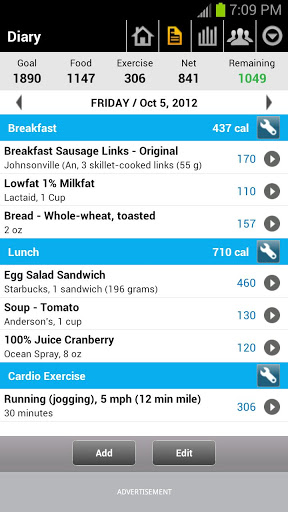
\includegraphics[width=0.9\textwidth]{ch2/RelatedApps/MyFitnessPal/1.jpg}
  }
\end{subfigure}%
\begin{subfigure}[b]{.33\textwidth}
  \centering
  \fbox{
  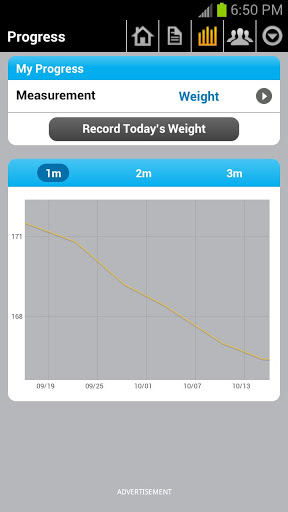
\includegraphics[width=0.9\linewidth]{ch2/RelatedApps/MyFitnessPal/2.jpg}
  }
\end{subfigure}
\begin{subfigure}[b]{.33\textwidth}
  \centering
  \fbox{
  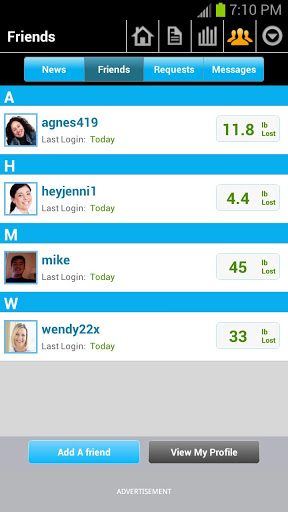
\includegraphics[width=0.9\textwidth]{ch2/RelatedApps/MyFitnessPal/3.jpg}
  }
\end{subfigure}%
}
\caption{Users' Food Diary (left). Users' Progress Report(middle). Users' friends activities (right).}
\label{fig:MyFitnessPal}
\end{figure}
\newpage
\item My Food
Circle\footnote{\href{https://play.google.com/store/apps/details?id=com.multipie.slimcircle}{Google
Play Store Application-My Food Circle}.} : This is a
social~\cite{North51digital} app that helps you instantly share pictures of what
you are eating with your friends. Through this you can connect with people and
friends or you can maintain private food diary.
This app is not only great fun but also can be a big help to stay healthy, lose
weight, eat for fitness, or just enjoy tasty nutritious food. This has also
functionalities like rate one another's meals and share comments, ideas,
encouragement and advice.
\begin{figure}[h!t]
\centering
\fbox{
\begin{subfigure}[b]{.33\textwidth}
  \centering
  \fbox{
  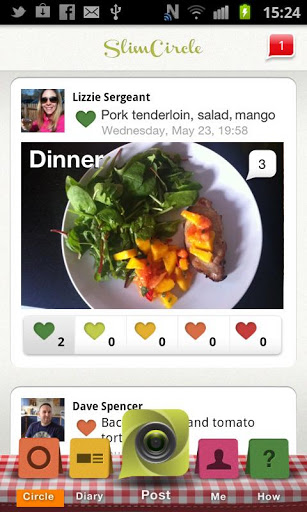
\includegraphics[width=0.9\textwidth]{ch2/RelatedApps/MyFoodCircle/1.jpg}
  }
\end{subfigure}%
\begin{subfigure}[b]{.33\textwidth}
  \centering
  \fbox{
  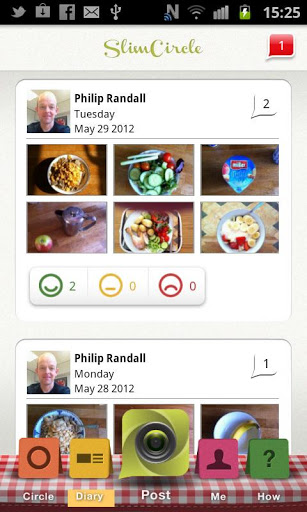
\includegraphics[width=0.9\linewidth]{ch2/RelatedApps/MyFoodCircle/2.jpg}
  }
\end{subfigure}
\begin{subfigure}[b]{.33\textwidth}
  \centering
  \fbox{
  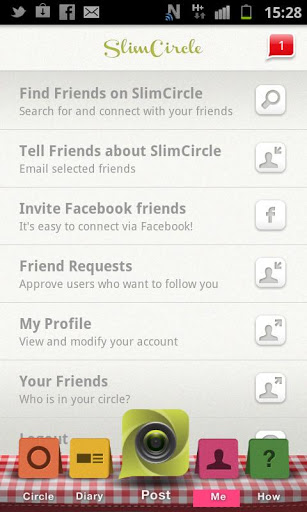
\includegraphics[width=0.9\linewidth]{ch2/RelatedApps/MyFoodCircle/3.jpg}
  }
\end{subfigure}
  }
\caption{Users' wall of My Food Circle (left). User's Food Diary (middle).  Users' functionalities of My Food Circle (right).}
\label{fig:MyFoodCircle}
\end{figure}

\item Restaurant
System\footnote{\href{https://play.google.com/store/apps/details?id=com.aadhk.restaurant}{Google
Play Store Application-Restaurant System}.} :
Restaurant System is a demo android application where customers could order
foods before going to restaurent and also can reserve a table. Waiters also can
use application to check orders from customers' and Chefs receives orders
directly, which are displayed in the monitors placed in the kitchen.

\begin{figure}[h!t]
\centering
\fbox{
\begin{subfigure}[b]{.33\textwidth}
  \centering
  \fbox{
  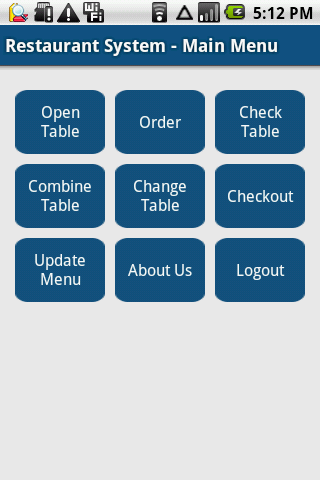
\includegraphics[width=0.9\textwidth]{ch2/RelatedApps/RestaurantSystem/1.png}
  }
\end{subfigure}%
\begin{subfigure}[b]{.33\textwidth}
  \centering
  \fbox{
  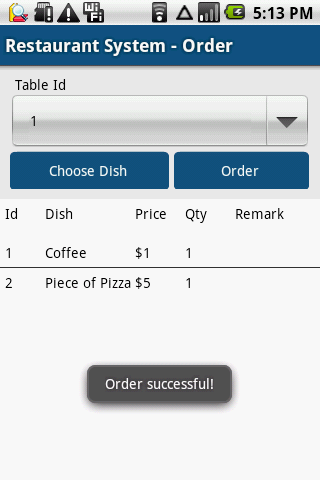
\includegraphics[width=0.9\linewidth]{ch2/RelatedApps/RestaurantSystem/2.png}
  }
\end{subfigure}
\begin{subfigure}[b]{.33\textwidth}
  \centering
  \fbox{
  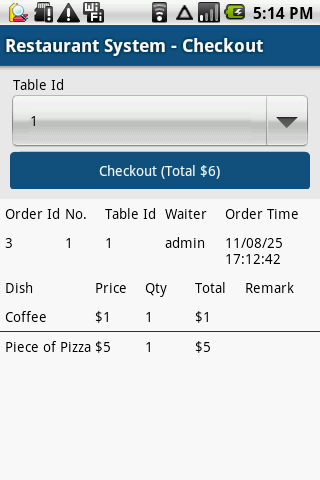
\includegraphics[width=0.9\linewidth]{ch2/RelatedApps/RestaurantSystem/3.png}
  }
\end{subfigure}
}
\caption{Users' Dashboard of Restaurant System(left). Restaurant System Order Dish(middle).  Restaurant System checkout Dish(right).}
\label{fig:RestaurantSystem}
\end{figure}

\end{enumerate}



\clearpage
\newpage
%\thispagestyle{empty}
\mbox{}
%\enlargethispage*{1000pt}

\chapter{Analysis of Smart Cafeteria}
\label{chap:AnalysisofSmartCafeteria}

In this chapter, I will explain the methodology
[\ref{sec:RequirementDataGathering}] and the result of analysis phase
[\ref{sec:DataAnalysis}] of ``Smart Cafeteria''. In the first section, I have
provided the definition of Requirements and Data Gathering techniques; and also
mentioned different data gathering techniques which were required to collect
requirements for ``Smart Cafeteria''. I have used some data gathering techniques
that are used to find and clarify the users' needs and requirements for ``Smart
Cafeteria''.


At the very beginning of analysis, I have started to study documents and
researched about ``Smart Cafeteria'' and found a set of stakeholders
[\ref{subsec:Stakeholders}], initial functional requirements [\ref{subsec:FR}]
and non functional requirements [\ref{subsec:NFR}].
Then I have studied Opera universitaria's documents related to Mensa and found a
few new requirements [\ref{subsec:MensaDocuments}]. To find out more
requirements for ``Smart Cafeteria'' I have made a focus group discussion
[\ref{subsec:FocusGroup}] and finally went through questionnaire
[\ref{subsec:Questionnaires}].


In the second section [\ref{sec:DataAnalysis}], I have presented data analysis and
result using previous set of requirements. The result was presented using UML
2.0 e.g. Use Case diagram [\ref{subsec:usecase}], Class Diagram
[\ref{subsec:classdiagram}] and Activity Diagram [\ref{subsec:activity}].


\section{Requirements and Data Gathering}
\label{sec:RequirementDataGathering}
\textbf{A Requirement} \cite{preece2002interaction} is a statement about a
proposed system that specifies what it should do or how it should perform it's
activities. One of the aim of the requirement activity is to make them as
specific, unambiguous, and clear as possible. Traditionally, there exists two
different kind of requirement; \textbf{functional requirements} which concerns
about what the system should do, and \textbf{non functional requirements} which
states about the constraints of the system and its development. The main reason
of the requirement analysis is to understand about the users, their work, and
the context , so that the system can be developed such a way which could satisfy
the requirements of the users. This is called identifying needs. On the other
hand, second aim is to produce a set of stable requirements that drive to next
phase which is design phase.
Identifying needs and establishing requirements is itself an iterative activity
in which the sub activities inform and refine one another. It does not last for
a precise number of weeks or months, it lasts until it achieves usability goals.

The purpose of \textbf{data gathering} is to find  a set of stable requirements
even though a set of initial requirement exists, data accumulation will help to
expand, clarify, and confirm those initial requirements. Data accumulation needs
to cover a wide spectrum of issues because the different kind of requirements
needed to be established~\cite{preece2002interaction}.

There are very few number of basic techniques to gather data, but they are very
important and flexible which could be combined and extended in many ways.
These will give scope to understand the  variety of requirements and these
techniques are commonly studying documentation, questionnaires, interviews,
focus groups and workshops, users' observation.

\subsection{Stakeholders}
\label{subsec:Stakeholders}
Stakeholders are the people from whom all requirements will be gathered, the
people who has the most influence on design and the people who will get 
benefited from the completed project. Here is the list of all stakeholders of the
smart cafeteria.
\begin{enumerate}
\item \textbf{System Users:} System user is those who are going to use and get
services from our system ``smart cafeteria''. They are usually students,
professors, researchers, University administration officers and University
technical staffs who are closely involved with our system. Their main goal is to
search food menu in online system application and order menu through online to
reduce mensa queue time.
\item \textbf{Students:} Students are one of the most important stakeholder who
belongs to system users. Basically most of the students are busy with their
classes, examinations and they stay at the university almost entire day and
generally take their breakfast, lunch and some cases even their dinner in
cafeteria.
\item \textbf{Professors:} Professors are one of the most important stakeholder
who will be system users. They are mostly busy with their classes, seminars,
projects in all day long at the university.
\item \textbf{Researchers:} Researchers are another kind of stakeholder and
system users who are going to use this system to get services.
\item \textbf{Administrative Officer \& Technical Staff:} University
administrative officers \& technical staffs are system users and stakeholder.
They stays busy with their work all day long and also take their lunch at
university cafeteria. So they will also get services and facilities from this
system.
% \item \textbf{University's Technical Staff:} University's technical staffs are
% system users and also will be one stakeholder of this system.
\item \textbf{System Administrator:} System administrator is a kind of
stakeholder of this system who is going to manage the system, update menu in the
system, check the order and add all kind of information related to cafeteria in
the system. Cafeteria staffs are the mainly system administrator and their main
goal is to spread food menu information through online.
\item \textbf{Cafeteria Staff:} They are one kind of stakeholder and a
kind of system administrator who is going to check the order and serve the menu
for the other stakeholders.
\end{enumerate}

\subsection{Initial Functional Requirements}
\label{subsec:FR}
As a cafeteria user I have done initial analysis and found some initial
functional requirements from my previous experience and knowledge  which is
discussed in this section. To find out more requirements and make the system
stable, I have studied cafeteria's food menu and related documents
[\ref{subsec:MensaDocuments}], built focus group [\ref{subsec:FocusGroup}] and
conducted interview with questionnaires [\ref{subsec:Questionnaires}].

In software engineering, a functional requirement defines the functions of a
software system and its component \cite{Karthika2012}. A function is described
as a set of input, it's behavior, and outputs. Functional requirements may be
calculations, technical details, data manipulation, processing and other
specific functionality that describes what a system will do. The system uses the
functional requirements that are captured in use cases. All functional
requirements are supported by non functional requirements which impose some
constraints  such as security, reliability, portability on the design and
implementation of the system. Functional requirement catches the proposed
behavior as services, tasks or functions of the system that is required to
achieve goals.

The functional requirements of ``Smart Cafeteria'' as follows which is
categorized by different roles and tasks in the application.
\begin{enumerate}[(I)]
\item \textbf{System Users:} System users have the principle role in the system
application. They are basically students, professors, researchers, university
administration officers and university technical staffs who are going to use the
system. After research, I have found the following functionalities of the system
users into the ``Smart Cafeteria'' which has been shown in table
\ref{tab:FRSystemUsers}.

\begin{table}[h!t]
\centering
%\captionof{table}{Usefulness} \label{tab:Usefulness} 
 \begin{tabular}{| p{2cm} | p{10cm} |}
    \hline
    Serial No. & Functional Requirements \\ \hline
    F1 & User should register in the system to get services. \\ \hline
    F2 & Registration confirmation through email. \\ \hline
    F3 & Forgot user name or password. \\ \hline
    F4 & Login into the system. \\ \hline 
  	F5 & Login into system through application login function. \\ \hline 
    F6 & Login into system through university's login service. \\ \hline 
    F7 & Check users own dashboard after login. \\ \hline 
 	F8 & User can update user's own information and credential (change profile information, password). \\ \hline
 	F9 & follow users. \\ \hline 
 	F10 & view User's activities. \\ \hline 
 	F11 & View list of food menu. \\ \hline 
 	F12 & Search food menu. \\ \hline 
 	F13 & View menu details. \\ \hline 
 	F14 & Place oder menu. \\ \hline 
  	F15 & Payment for order. \\ \hline 
   	F16 & View order statistics. \\ \hline
   	F17 & View dieting report and calorie consumption per day. \\ \hline
   	F18 & Generate dieting report. \\ \hline
   	F19 & Rating in food menu . \\ \hline
   	F20 & Give comments in individual food menu. \\ \hline
   	F21 & Generate report. \\ \hline 
   	F22 & Take food menu receipt after placing order by punching student card into the POS terminal. \\ \hline 
    \end{tabular}
 \caption{Functional Requirements of System Users.}
\label{tab:FRSystemUsers}
\end{table}

\item \textbf{System Administrator:} System administrators who are basically
cafeteria's staffs have the following functionalities that has been shown in the
table \ref{tab:FRSystemAdministrator}.

\begin{table}[h!t]
\centering
%\captionof{table}{Usefulness} \label{tab:Usefulness} 
 \begin{tabular}{| p{2cm} | p{10cm} |}
    \hline
    Serial No. & Functional Requirements \\ \hline
    F23 & Login in admin panel. \\ \hline
    F24 & Add food menu in the system. \\ \hline
    F25 & Edit food menu. \\ \hline
    F26 & Delete food menu. \\ \hline 
  	F27 & Manage order. \\ \hline 
    F28 & View order. \\ \hline 
    F29 & View order statistic per day (Total order). \\ \hline 
 	F30 & View order statistic per week. \\ \hline
 	F31 & View order statistic by menu. \\ \hline 
 	F32 & view User's activities. \\ \hline 
  	F33 & Search order by food menu. \\ \hline
  	F34 & Search food menu by name and key word. \\ \hline 
  	F35 & Generate report. \\ \hline 
    \end{tabular}
 \caption{Functional Requirements of System Administrator.}
\label{tab:FRSystemAdministrator}
\end{table}

\item \textbf{System Application:} System application itself has some
functionality which has to be performed to make the system more interactive. The
functionalities of system application has been shown in table
\ref{tab:FRSystemApplication}.

\begin{table}[h!t]
\centering
%\captionof{table}{Usefulness} \label{tab:Usefulness} 
 \begin{tabular}{| p{2cm} | p{10cm} |}
    \hline
    Serial No. & Functional Requirements \\ \hline
    F36 & Generate daily food menu notification through email or sms. \\ \hline
    F37 & Generate weekly food menu notification to users. \\ \hline
    F38 & Suggesting list of food menu to users based on their choice rating and
which food menu they have took daily and how much calorie they have took in the last
couple of weeks. \\ \hline
    F39 &  Order status will be kept pending until user takes the receipt from POS
terminal. \\ \hline 
  	F40 & Order status confirm after users take food menu receipts by punching
student card. \\ \hline 
    \end{tabular}
 \caption{Functional Requirements of System Application.}
\label{tab:FRSystemApplication}
\end{table}

\item \textbf{POS Terminal:} POS terminal is used for payment through master
card in most of shops or supper market. But in ``Smart cafeteria'' it could be
used to pay or print order receipt after order food and successfully paying
online. The POS terminal has some functionalities which has shown in the table
\ref{tab:FRPOSTerminal}.

\begin{table}[h!t]
\centering
%\captionof{table}{Usefulness} \label{tab:Usefulness} 
 \begin{tabular}{| p{2cm} | p{10cm} |}
    \hline
    Serial No. & Functional Requirements \\ \hline
    F41 & Print food menu order receipt after punching card into the POS terminal machine. \\ \hline
    F42 & Send a notification to the system that user got the receipt after order. \\ \hline
       \end{tabular}
 \caption{Functional Requirements of POS Terminal.}
\label{tab:FRPOSTerminal}
\end{table}
\end{enumerate}

\subsection{Non Functional Requirements}
\label{subsec:NFR}
Non functional requirement defines sometimes as system qualities and properties
of the system such as performance, security, maintainability in order to support
functional requirements. In other words, how well some behavioral or structural
view of the system could be accomplished.
The ``IEEE-Std 830 - 1998"\footnote{ IEEE Std 830-1998, Recommended Practice for
Software Requirements Specifications IEEE Recommended Practice for Software
Requirements Specifications} has discussed some non-functional
requirements~\cite{Committee1998} in a Software Requirements Specification and
after research, I have found the following non functional requirements for
``Smart Cafeteria'':
% \begin{itemize}

\renewcommand{\labelenumi}{\arabic{enumi}.}
\renewcommand{\labelenumii}{(\roman{enumii})}


\begin{enumerate}

\item \textbf{Usability:} Usability is the most important non functional
requirement in smart cafeteria project and our main focus is on system usability
from non functional requirements along with the functional requirements of the
system. Usability is the activities with which a user can learn to operate,
easily understand inputs for and outputs of the system or component. From
previous discussion \ref{sec:HeuristicsUsability}, usability is generally
regarded as ensuring that interactive systems are effective to use, easy to
learn and enjoyable from user's perspective. Our system should also hold the
usability heuristics principles which is discussed earlier.

\item \textbf{Internationalization:} Since students in the University of Trento
are from various cultures and speakes different languages, our proposed system
should support multi language interfaces and functionalities.

\item \textbf{Portability:} The proposed system will be portable since the
system application will be accesable from Desktop PC, Laptop, Tablet as well as
Smart phone. This application will definitely support the non functional
requirement ``portability''.

\item \textbf{Adaptability:} According to \citet{Subramanian2001}, adaptation of
software systems is an unavoidable process which needs faster development of new
 or maintenance of existing software systems  due to the change in customer
requirements. There are also several definitions of adaptability which are taken
from several papers; some of those definitions are described bellow:
\begin{enumerate}
\item  According to ~\citet{Oreizy:769885:Gorlick}, ``Self-adaptive software
modifies its own behavior in response to changes in its operating environment''.

\item  ``Adaptability is defined as the ease with which a system or parts of the
system may be adapted to the changing
requirements~\cite{Subramanian2001,Tekinerdogan}.''

\item  ``A program is called adaptable if it can be easily changed. A program is
called adaptive if it changes its behavior automatically according to its
context~\cite{Subramanian2001,Lieberherr1995}".
\end{enumerate}
There are several things of software adaptation in our proposed smart cafeteria
system and one of them is the system capable of accepting http/https request
from different clients such as desktop, tablet as well as different versions OS
of smart phone and respond to them as well.


\item \textbf{Safety and security:} Safety and security is heighly important
non functional requirements of a system. There are some safety
and security non functional requirements propose in our smart campus
project and those are as follows:
\begin{enumerate}
\item  Our proposed system ensures authorized access to the system data as well as
user information.
\item The communication between the application server and client must be
encrypted and use https protocol.
\item Backup of all the system data should be taken every 24 hours and it should
be saved in a secure location.
\item System makes sure to stop if there is a any probability of security attacks.
\end{enumerate}

\item \textbf{Reliability:} In the software requirements specification
(SRS)\footnote{ IEEE Std 830-1998, Recommended Practice for Software
Requirements Specifications.}, Reliability is the most common non functional
requirement. There are some proposed non functional requirement for reliability in
our smart campus project and those are as follows:
\begin{enumerate}
\item	System should be available 24 hours.
\item	System should not have any failure during operation.
\item	Good reputation towards user.
\item	Deliver such services and functionalities that user can trust.
\end{enumerate}
\item \textbf{Performance:} Performance is a common non functional
requirement for a system. The following things should be available in our
system as non functional requirements:
\begin{enumerate}
\item Speed should be good in the operation of the system.
\item Response time of the operation should be good in any platform e.g. in
desktop, tablet, smart phone.
\end{enumerate}

\item \textbf{Documentation Requirements:} According to Software Requirement
Specification, ``Smart Cafeteria'' will specify and maintain proper
documentation before the start of development. The document should contain Title
and Author, scope, stakeholder, functional requirements, usability requirements,
technical requirements accordingly IEEE Std.

\end{enumerate}


\subsection{Studying Cafeteria's Food Menu and Documents}
\label{subsec:MensaDocuments}
Studying documentation is an important part of data gathering technique.
Procedures and rules are written down sometimes in manuals or papers and these
are a good source of data. In the requirement activity, studying documentation
is good for understanding legislation and getting some background information
about the work as well as the system~\cite{preece2002interaction}. Since
studying documents is essential, I have researched and studied about Mensa's
food menu [ Figure \ref{fig:differentmenu}] and Mensa's other documents
[Appendix~\ref{sec:MenuAppendix}] of Opera Universitaria di
Trento~\cite{operauniversity}(university of Trento).
\begin{figure}[h!t]
    \centering
      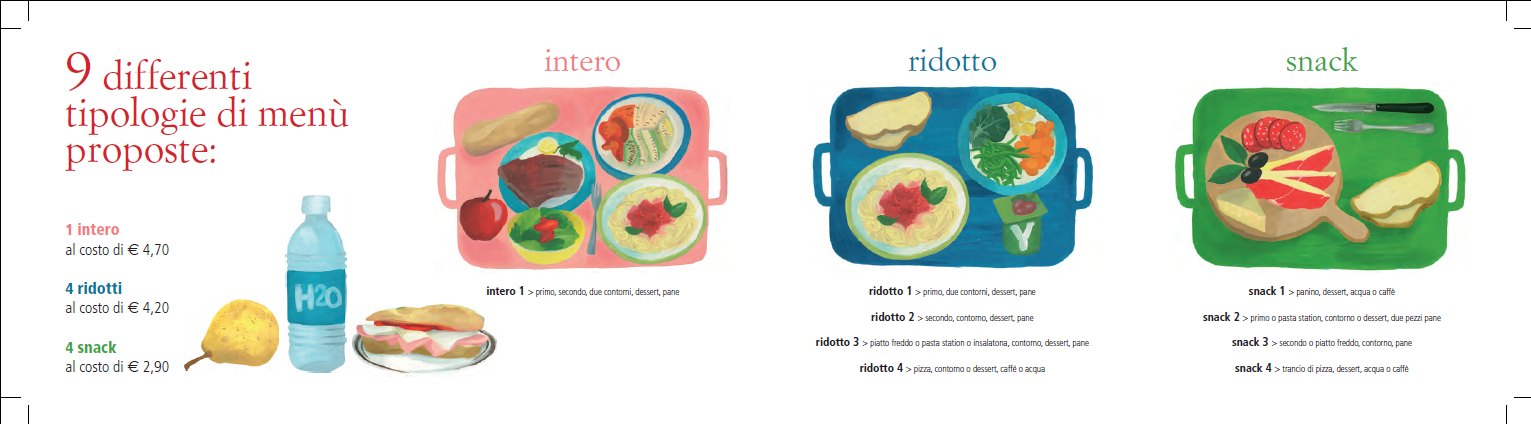
\includegraphics[width=5.5in,height=2in]{ch3/AppendixMenu/differentmenu}
  \caption{different menu of Mensa in University of Trento.}
  \label{fig:differentmenu}
\end{figure}
From this research, I have found the following facts:
\begin{itemize}
\item Since university of Trento has several departments in the several places,
university has a lot of cafeteria branch in different place as well.
\item I have also found that all cafeteria branches have a monthly opening time
schedule in the website as a pdf document.
\item I have also found each cafeteria offers different food menu such as full
menu, reduce menu and snack charging of different prices and where each menu contains
different food items and calories as well.
\end{itemize}
From those of facts, I have come down into a decision and added some more
functional requirements into the system. The additional functional requirements
as follows:\\ \\
\textbf{System administrator}
\begin{enumerate}
\item System administrator can add, edit and delete operation into the
system for cafeteria branch.
\item System administrator can add, edit and delete monthly operating time
schedule of each branch into the system; for example, povo1 is closed January 1
to January 6, 2013 and others working days of the month January 2013 will be
opened.
\item System administrator can add, edit and delete food item which contains
food item status e.g. first course, second course, dessert, side dishes, cold
drinks, etc. and their respective Kilo calories per 100gm and other
information's.
\end{enumerate}
\textbf{System users}
\begin{enumerate}
\item System users can see and browse the cafeteria branches and monthly
operating time schedule of each branch respectively.
\item System user can create own menu using menu wizard from different food
items depending on their choice which may have different cost depending on food
items.
\end{enumerate}

\subsection{Focus Group}
\label{subsec:FocusGroup}
Focus group and workshop is a very good technique to gather data and set of
requirements. Interview is a such kind of thing which tends to be one on one
perspective where as focus group and workshop is a very effective, alternative
and collaborative technique to get a group of stakeholders together to discuss
about the system and find out set of requirements. This activity sessions should
be very structured with predefined set topics for discussion and I was as a
facilitator in that focus group session and I have discussed and asked several
questions[Appendix~\ref{sec:DataGatheringQuestionnaire}] about our smart
cafeteria system and its facilities and functionalities.
The participants took part in open discussions as well as gave answers to the
questionnaires \cite{preece2002interaction}.

There were 7 participants in this session, all of them are the student of
University of Trento who used to take their lunch in University's cafeteria.
In the Table \ref{tab:FocusGroup} [Appendix~\ref{sec:AppendixFocusGroup}] , the
summary of the focus group meeting are shown.

\begin{table}[h!t]
\centering
%\captionof{table}{Usefulness} \label{tab:Usefulness} 
 \begin{tabular}{| p{3cm} | p{4.5cm} | p{4.5cm} |}
    \hline
    Agenda Item & Discussion &  Decision\\ \hline
    
    Smart Cafeteria Functional Requirements & We discussed all functional
    requirements that I have found earlier. & They agree with all functional
    requirements and they suggested one extra functional requirements which is
    mobile application should support QR BARCODE. \\ \hline
    
    Smart Cafeteria Non Functional Requirements & We have discussed all non
    functional requirements from IEEE-Std 830 - 1993'.& All participants strongly
    supported Internationalization, Usability and Portability.\\ \hline
   
    Smart Cafeteria in mobile and Tablet apps & Now we are in the age of
    informational technology, especially in mobile computing phase where all
    applications drive to support in mobile and tablet in smartly. & All
    participants strongly supported smart cafeteria mobile applications.\\ \hline
    
    Adaptive mobile application & Adaptive application will observe user
    behavior, test, and user's psychology and conclude a result with the help of
    machine learning techniques and finally suggests a list of solutions. & All
    participants strongly supported smart cafeteria mobile applications which
    must be adaptive application.\\ \hline
       \end{tabular}
 \caption{Focus Group Discussion Summary.}
\label{tab:FocusGroup}
\end{table}

From the discussion, I have found requirements that, since the application also
supports mobile plateform, so the application could scan QR BARCODE
[Figure-~\ref{QRBARCODE}] which along with food menu automatically it forces to
order menu phase. In the [Appendix~\ref{sec:DataGatheringQuestionnaire}], the
questions asked to participants is shown.

\begin{figure}[h!t]
    \centering
      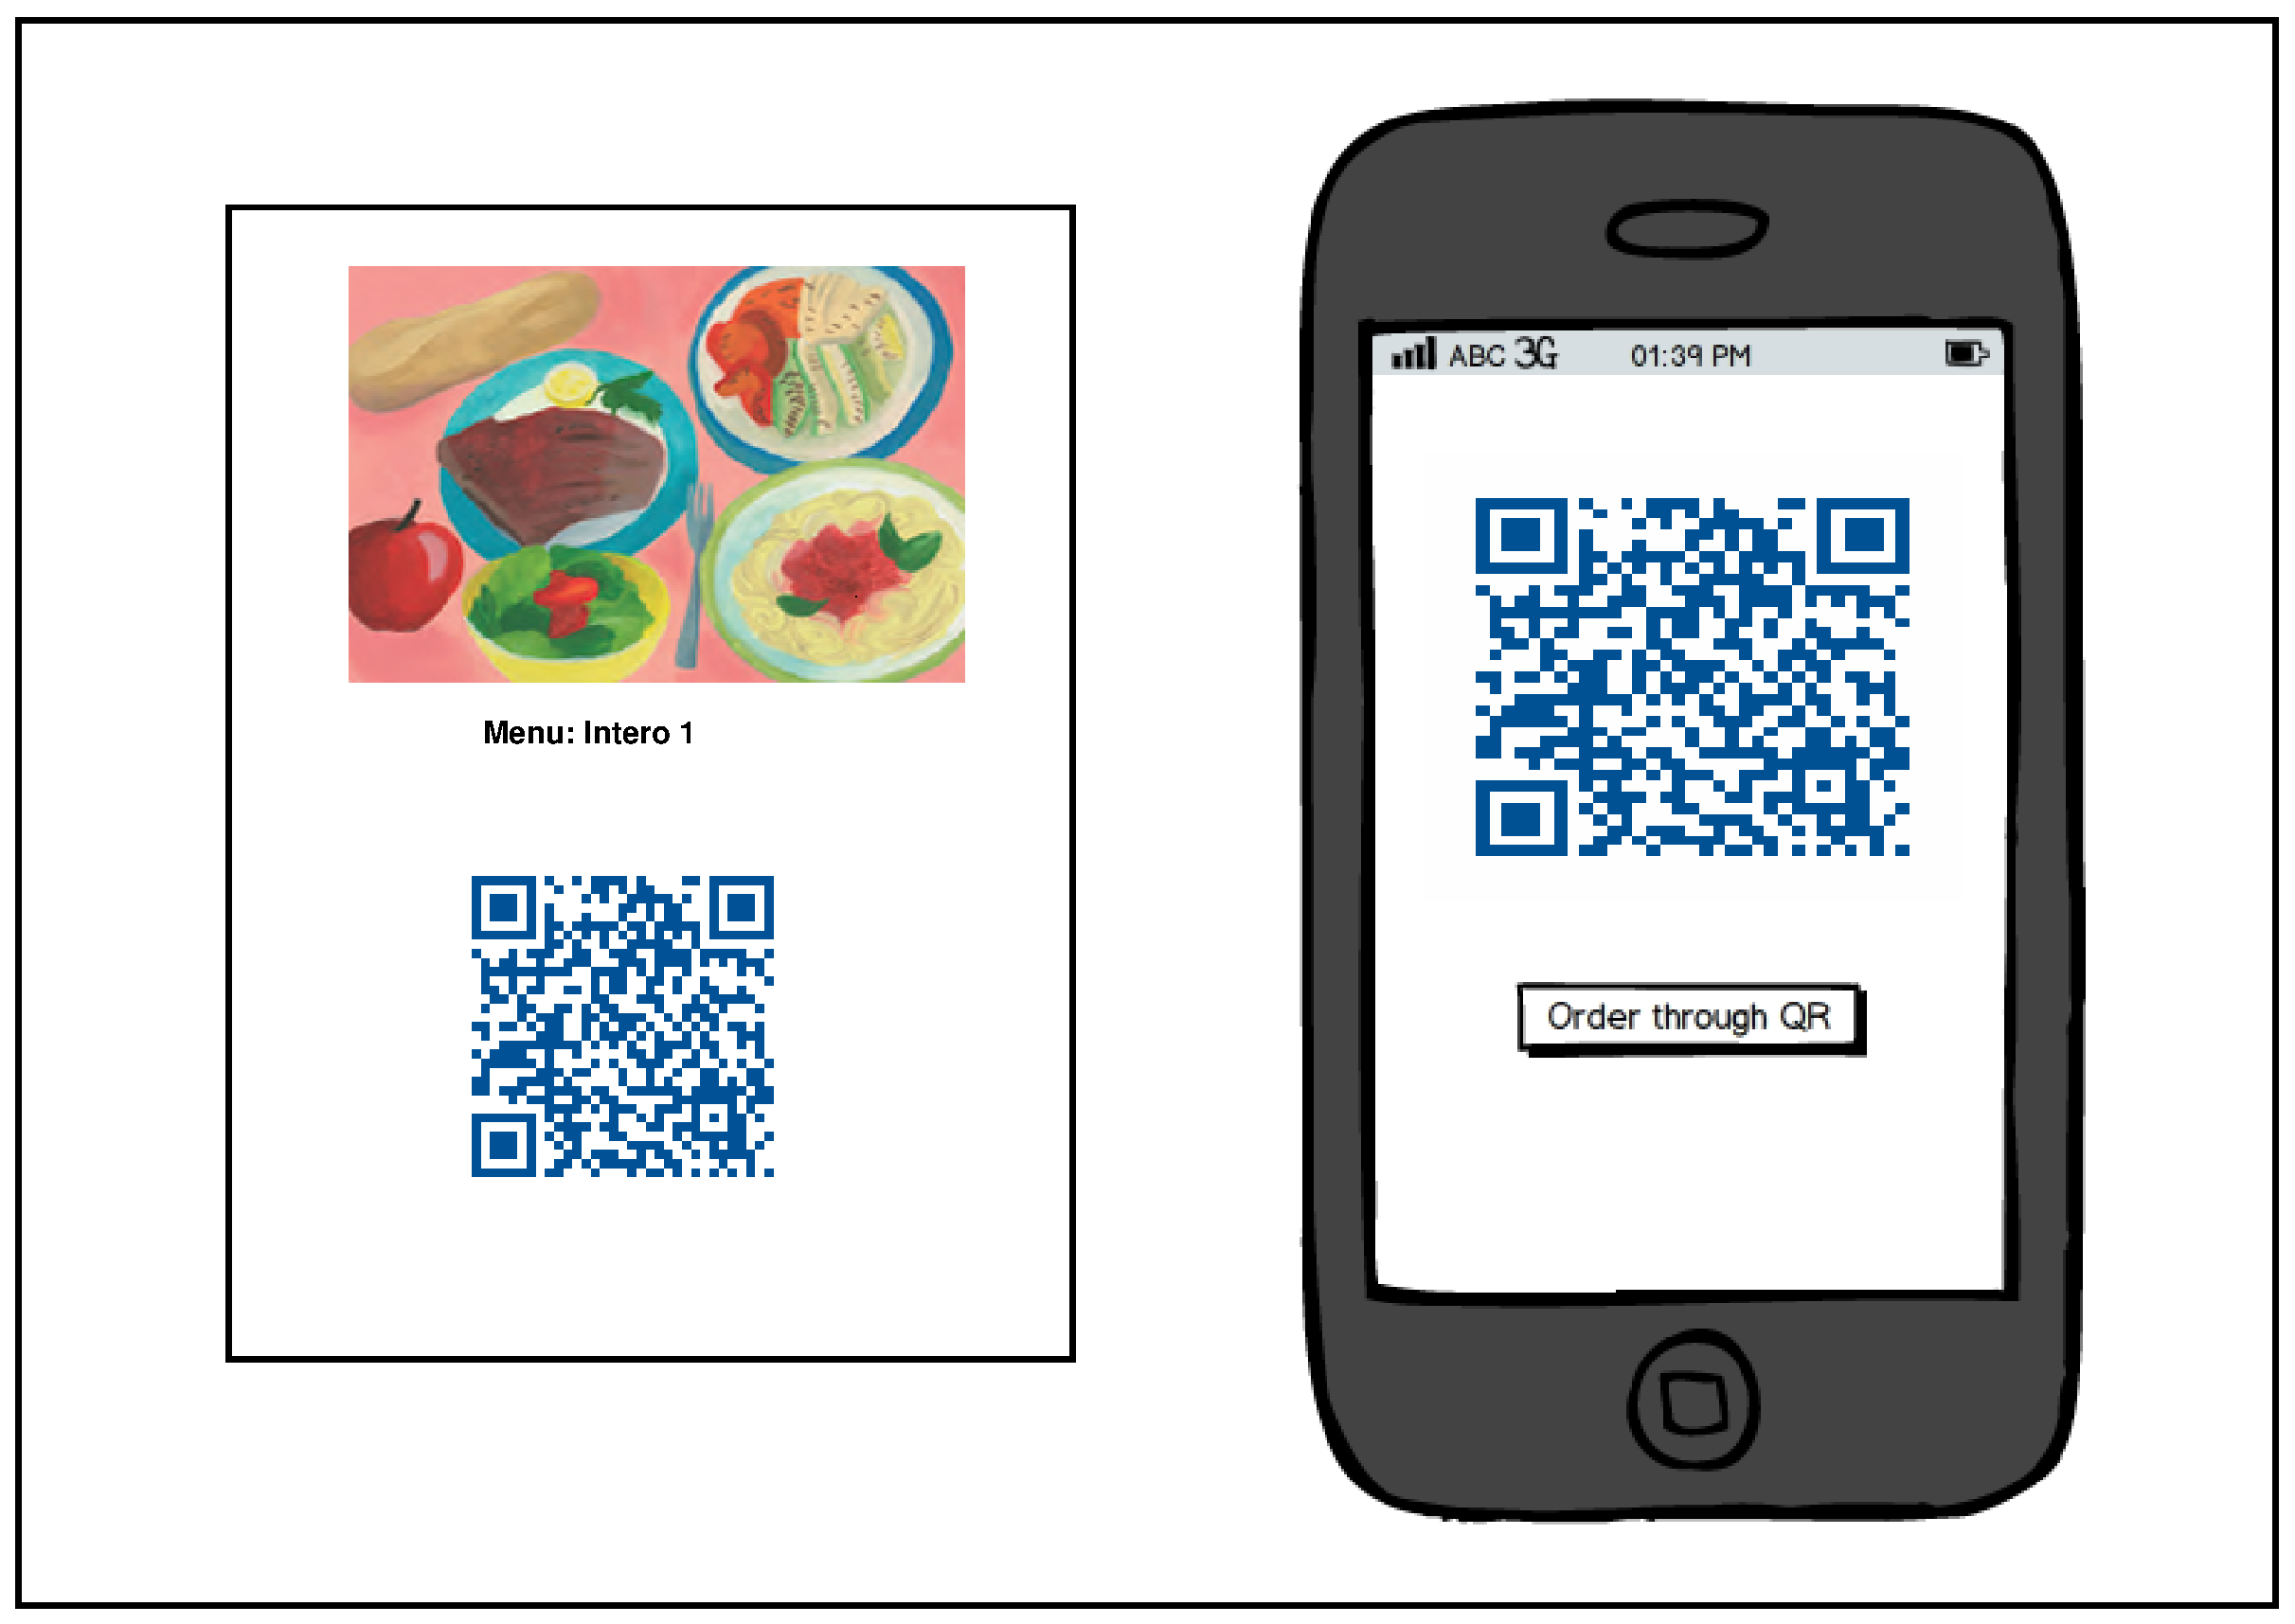
\includegraphics[width=5.5in]{ch3/FocusGroup/QRBARCODE}
  \caption{QR BARCODE}
  \label{QRBARCODE}
\end{figure}

\subsection{Questionnaires}
\label{subsec:Questionnaires}
\citet{AdamsAnneandCox2008} have defined that Questionnaires are usually paper
based or delivered online and consist of a set of questions which all
participants are asked to complete. Questionnaire is a kind tool that should be
easily understandable, interpretable; and should avoid complex words.
Questionnaires should hold reliability and validity; to increase the
effectiveness of questionnaires it is important that how it is structured and
it's unambiguity. Questionnaires should preserve interviewers' trust, privacy
and ethics; so interviewer should ensure confidentiality.
They also found that if a large number of users are participating, there
always have a chance to get a large amount of data which need to be coded and
analysed. They also suggested that focus group is better than conducting
single interview since interviews are usually conducted on a one-to-one basis.
It requires a large amount of the investigator's time during the interviews as
well as  transcribing and analyzing the data.

There were seven questions whose scale was based upon the Likert scale Effective
or not Effective and yes or no. On the other hand, two questions were for open
suggestions to improve the system's functionalities. The Table
\ref{tab:DataGatheringQuestionnaire}
[Appendix~\ref{sec:DataGatheringQuestionnaire}] has shown the questionnaire
which have asked to participants in focus group meeting and the number of
participants agreed or disagreed with the facts from total 7 participants.

\begin{table}[h!t]
\centering
%\captionof{table}{Usefulness} \label{tab:Usefulness} 
 \begin{tabular}{| p{8.5cm} | p{2cm} | p{2cm} |}
    \hline
    Questions/Answer & Yes or Effective &  No or Not Effective\\ \hline
    
    Do you support if an application which will provide mensa system where avoiding
    a long queues and saving time? & 7  & 0 \\ \hline
    
    If there will be an application where you could browse food menu, search
    food menu, order and pay online, then how effective the system will be ? & 7
     & 0 \\ \hline
    
    If the application let you create your own food menu as real
    scenario, how effective the system will be for you? & 5 & 2 \\ \hline
    
    how effective the system will be if the application supports mobile
    plateform? & 6 & 1 \\ \hline
    
    If the application could suggest you food menu depending on your choice,
    test, your dieting preferences, then how effective the system will be?  &
    7 & 0 \\ \hline
    
    If the application provides support in different languages, then how
    effective the system will be? & 7 & 0 \\ \hline
    
	Do you think that this application may help you or make your university life
	easier?  & 6 & 1 \\ \hline	

\end{tabular}
 \caption{Data Gathering Questionnaire \& Result.}
\label{tab:DataGatheringQuestionnaire}
\end{table}


\section{Data Analysis}
\label{sec:DataAnalysis}
Data interpretation and analysis is a very important part in the interactive
system development life-cycle. When Data-gathering session has been almost
finished, data interpretation and analysis phase could start and it is an
iterative step between data gathering and data analysis.

In data analysis~\cite{preece2002interaction}, different techniques and
notations were followed to find different aspects of the system that will give
different requirements. Traditionally, functional requirements have been
analyzed and expressed using data-flow diagrams, state charts diagram, work-flow
charts. Since our system development is using object-oriented approach,
functional and data requirements are combined in class diagrams and behavior of
the system being expressed using sequence diagrams. Use case focuses on goals of
users which were introduced through the object-oriented community . Use case
focuses specifically on the interaction between the user and a software system.
The term scenario is also used in the context of use cases.

In the following Subsections~\ref{subsec:usecase},~\ref{subsec:classdiagram}
and~\ref{subsec:activity} , I will describe and discuss about Use case diagrams,
Class diagram and Activity diagrams of ``Smart Cafeteria'' respectively.

\subsection{Use Case Diagram}
%\phantomsection
\label{subsec:usecase}
According to UML 2.0  specification~\cite{UML:2007:Specification}, a use case
diagram represents the relationship between actors and use cases within a
system. The use cases represent functionality of a system or a classifier as
like a subsystem or a class, as manifested to external integrator with the
system or the classifier. A use case diagram contains a set of actors, set of
use cases, some interfaces; and shows the relationships between these elements.
The relationships are mainly associations between the actors and the use cases;
generalizations, extend and includes among use cases; and generalizations
between the actors.

Since I have discovered some stakeholders and their goals in this system after
analysis, depending on those I have found four use cases scenarios. Bellow I
will describe those use case scenario one by one.

\subsubsection{Use case of System users}

In this use case, students, professors, researchers, university staffs all are
generalized as system user basically who are going to use the system to get some
service from ``Smart Cafeteria'' system.
System user can perform basic operation like registration, confirm registration,
forgot password, login and logout. Login could be performed through university's
authentication service and its own application login. After login into the
system users could access their own dashboard from where they could perform
search food menu, view list of food menu, view individual food menu, rating in
food menu, comments on food menu, place order food menu, change user's profile,
view dieting report. Through this system, users could also make their own food
menu using create menu wizard. System user could also see information about
cafeteria branches and their time schedule through the system. After order and
payments, system users must take a menu receipt after punching their card in the
POS terminal.

\begin{landscape}
\begin{figure}[h!t]
    \centering
    \fbox{
      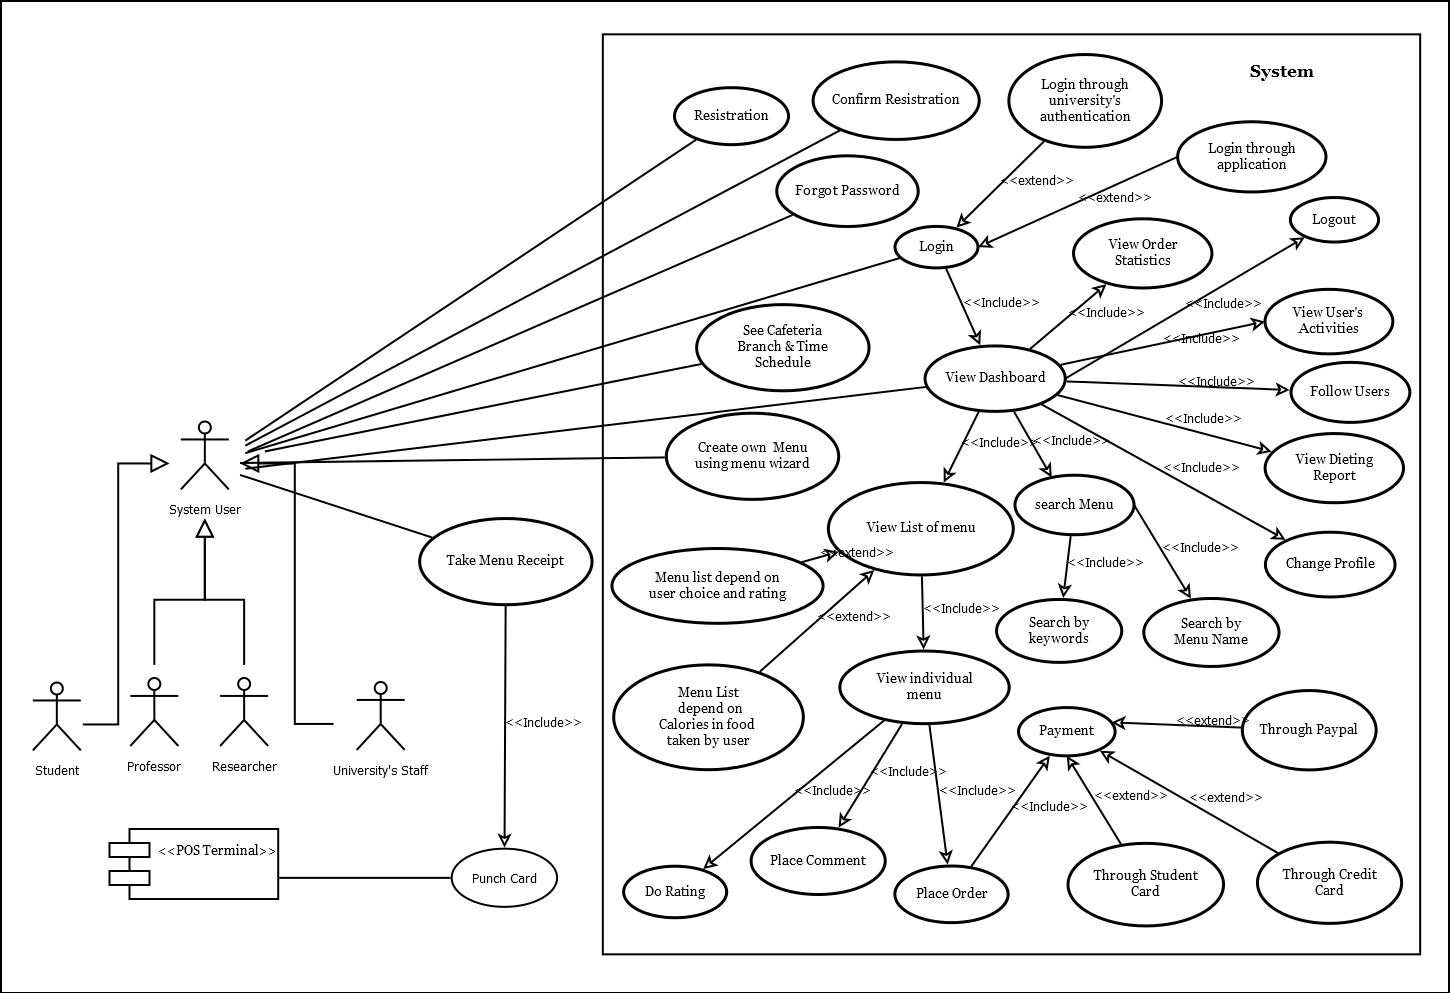
\includegraphics[width=8in]{ch3/UseCase/SystemUser}
      }
  \caption{Use Case Diagram of System User}
  \label{UCSystemUser}
\end{figure}
\end{landscape}

\subsubsection{Use case of System Administrator}

In the use case of system administrator, cafeteria staff's are generalized as
system administrator.
System administrator can perform their operation after login into the system.
After login, system administrator can access administrator dashboard. And from
administrator dashboard, system administrator can manage cafeteria branch which
means add, edit, delete and view operation on cafeteria branch and their
respected time schedule. System administrator can add, edit, delete and view
operation on food item and menu.
They also can make food menu from food item and menu. System user can view order
statistics, view total order, view order pending, generate various kind of
report.
\begin{figure}[h!t]
    \centering
      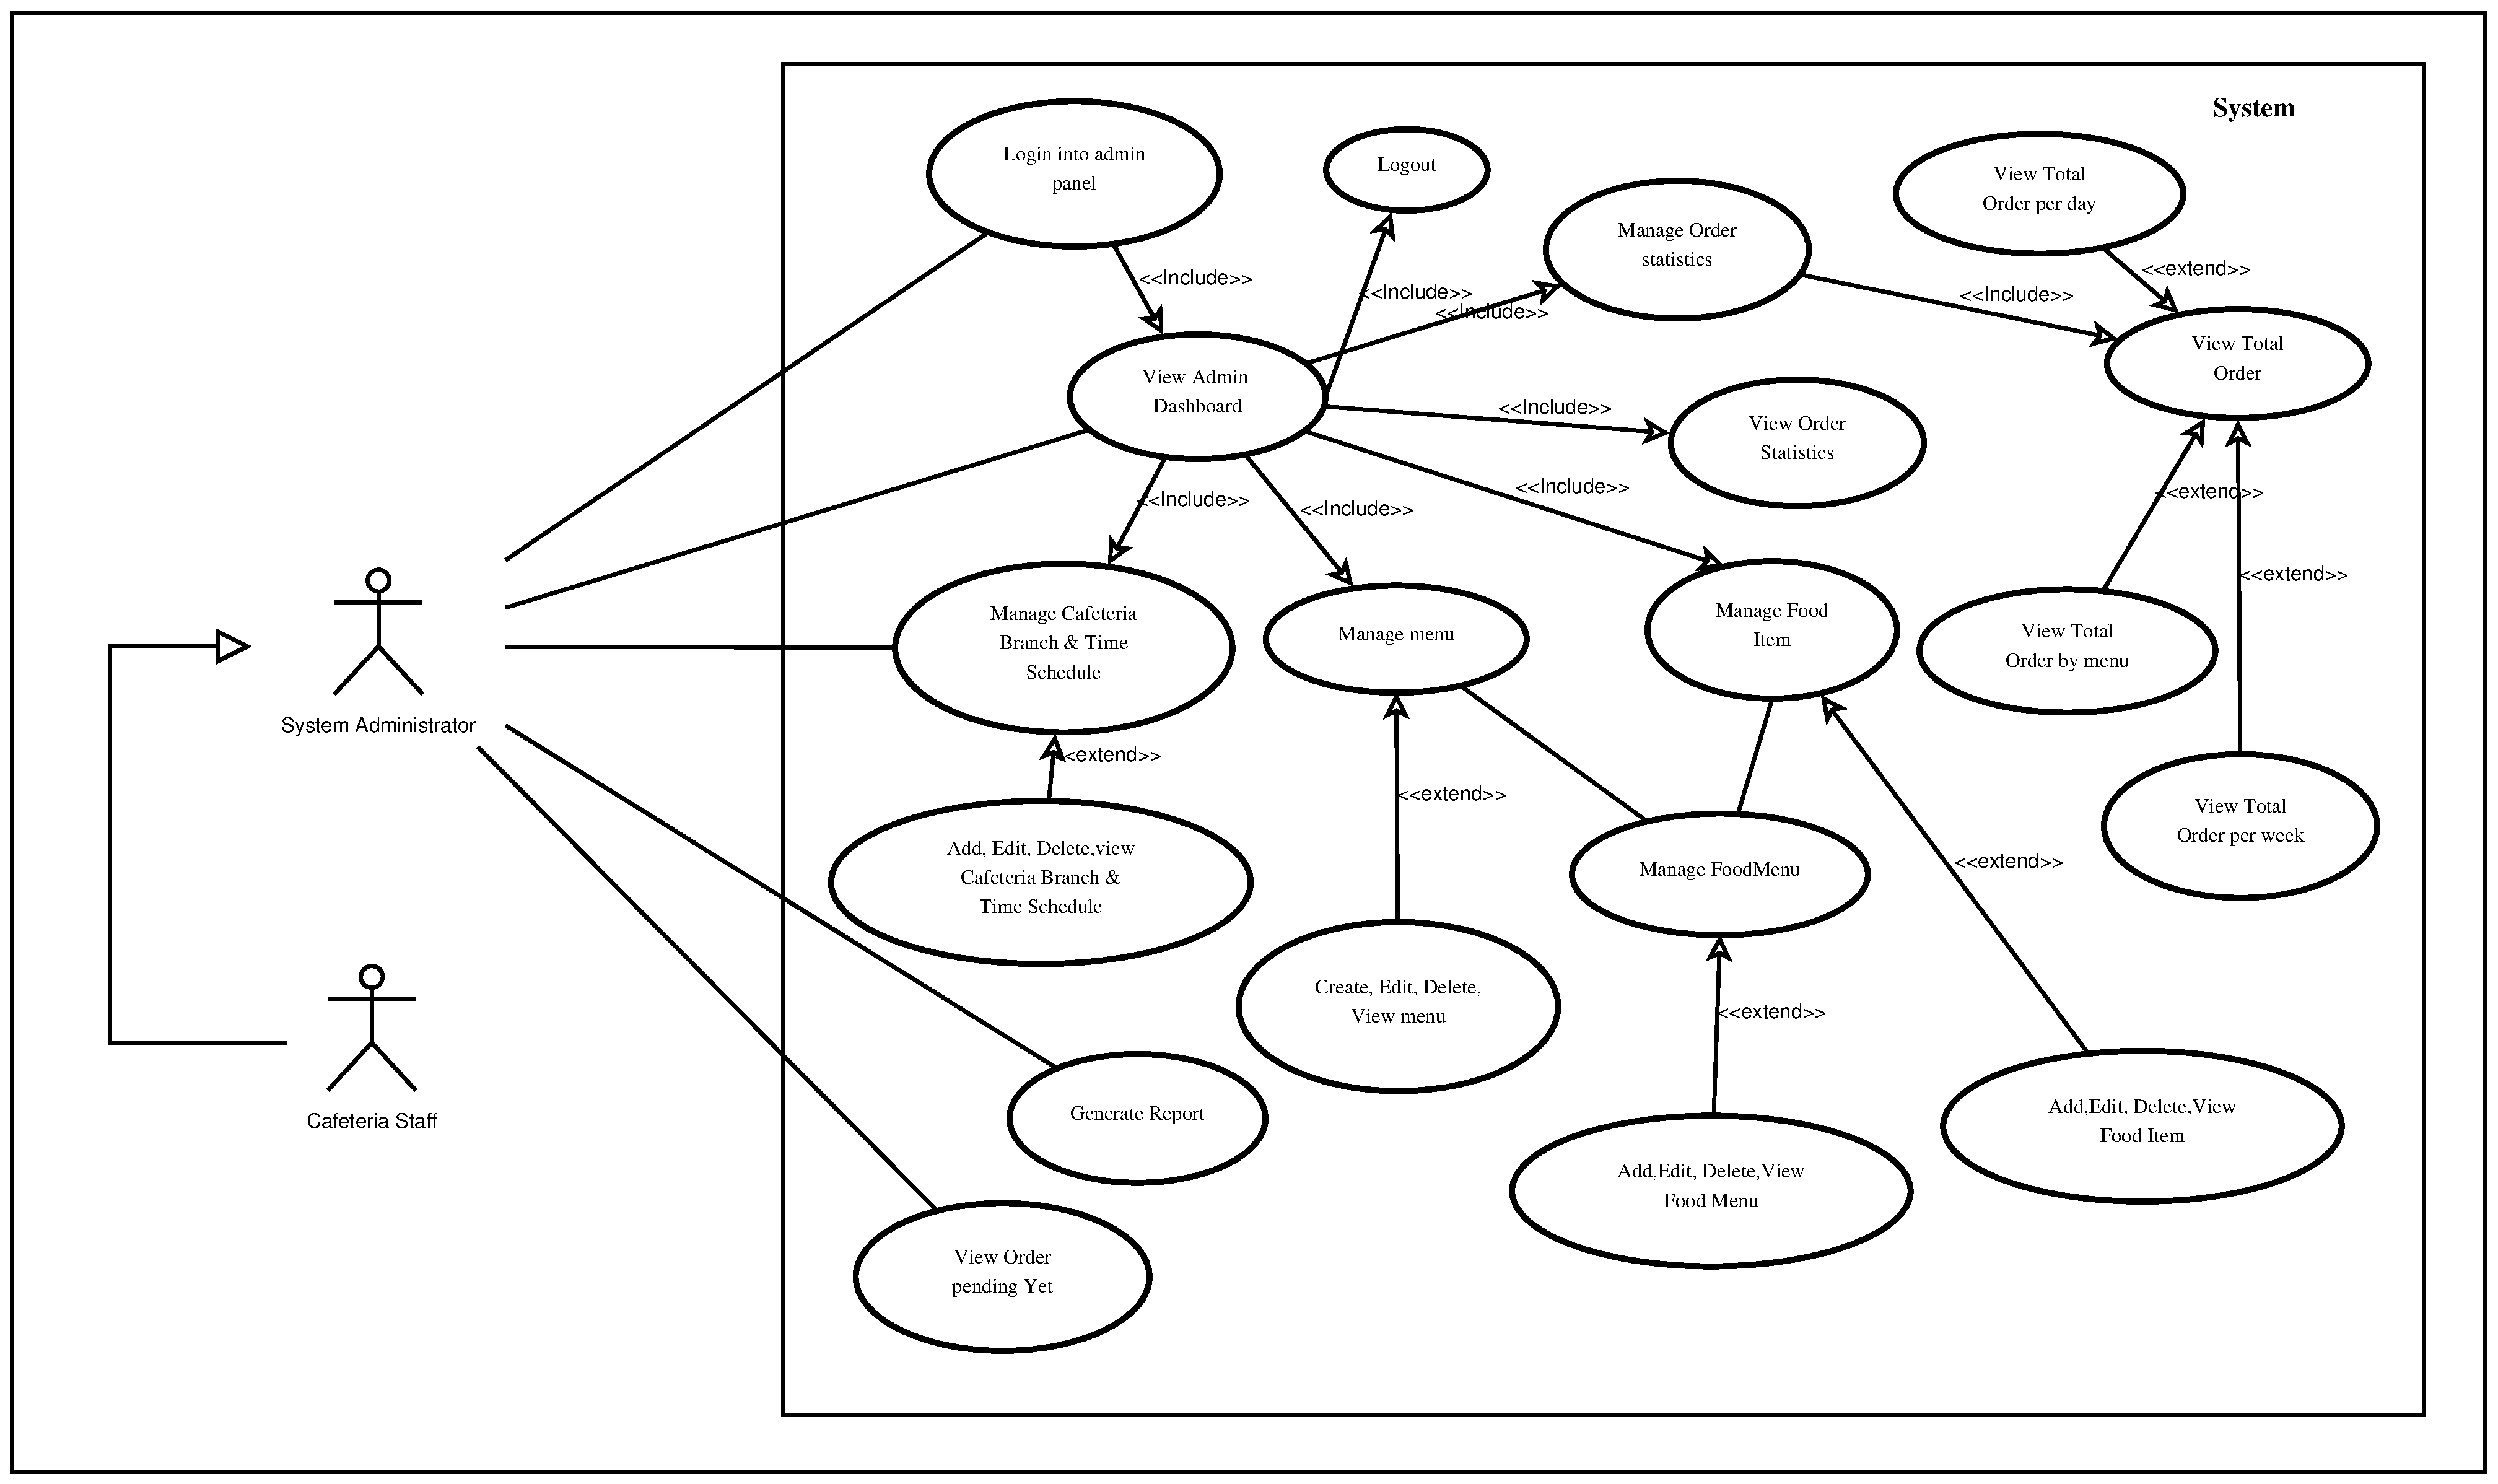
\includegraphics[width=5.5in]{ch3/UseCase/SystemAdministrator}
  \caption{Use Case Diagram of System Administrator}
  \label{UCSystemAdministrator}
\end{figure}

\subsubsection{Use case of System Application}

System application itself is a use case where generates various notifications
and sends to the system users either through using sms or email depends on user
preferences. System application also generates different list of food menu for
different user depending on their choices and calorie consumption of the last
couple of days. System application also make the order status pending until user
takes receipt from POS terminal  and also make the order status confirm when
user prints invoice from POS terminal punching the card.
\begin{figure}[h!t]
    \centering
      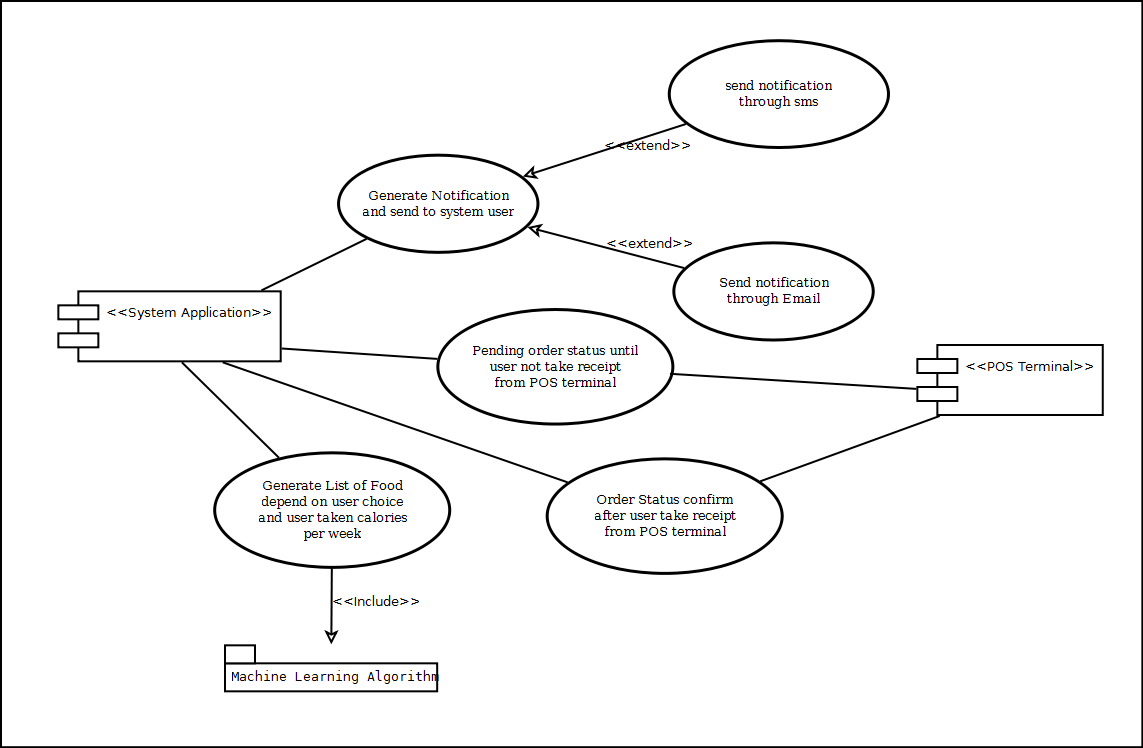
\includegraphics[width=5.5in]{ch3/UseCase/SystemApplication}
  \caption{Use Case Diagram of System Application}
  \label{UCSystemApplication}
\end{figure}

\subsubsection{Use case of POS terminal}

In the use case of POS terminal, POS terminal prints menu invoice for the system
user after he punches the card into the pos terminal after placing order for
food menu. When system user prints food menu receipt, POS terminal sends a
confirmation message to system application.
\begin{figure}[h!t]
    \centering
      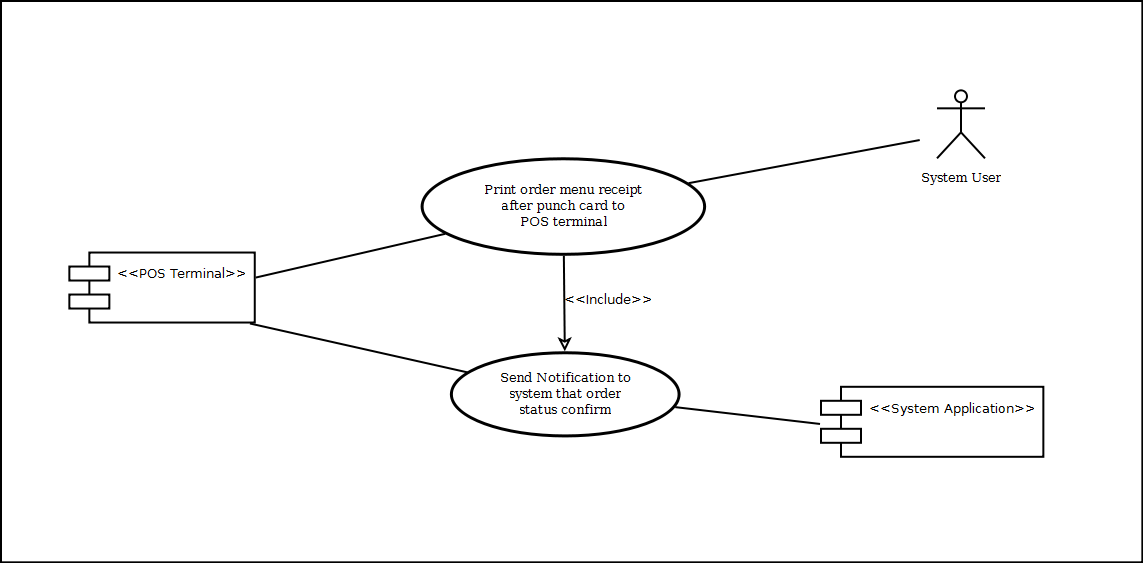
\includegraphics[width=5.5in]{ch3/UseCase/PosTerminal}
  \caption{Use Case Diagram of Pos Terminal}
  \label{UCPosTerminal}
\end{figure}
\newpage

\subsection{Class Diagram}
\label{subsec:classdiagram}
In UML 2.0 \cite{Donald} there are two basic categories of diagrams:
structure diagrams and behavior diagrams. Class diagram belongs to structure
diagrams which shows the static structure of the system which is going to be
modeled. In an object oriented application development, class diagram is very
important in initial stage to model a system. Each class consist attributes,
operations and relationships with other classes. In the following
figure~\ref{ClassDiagram}, I have modeled the class diagram of Smart cafeteria
and provided some description of each class.

\begin{landscape}
\begin{figure}[h!t]
    \centering
      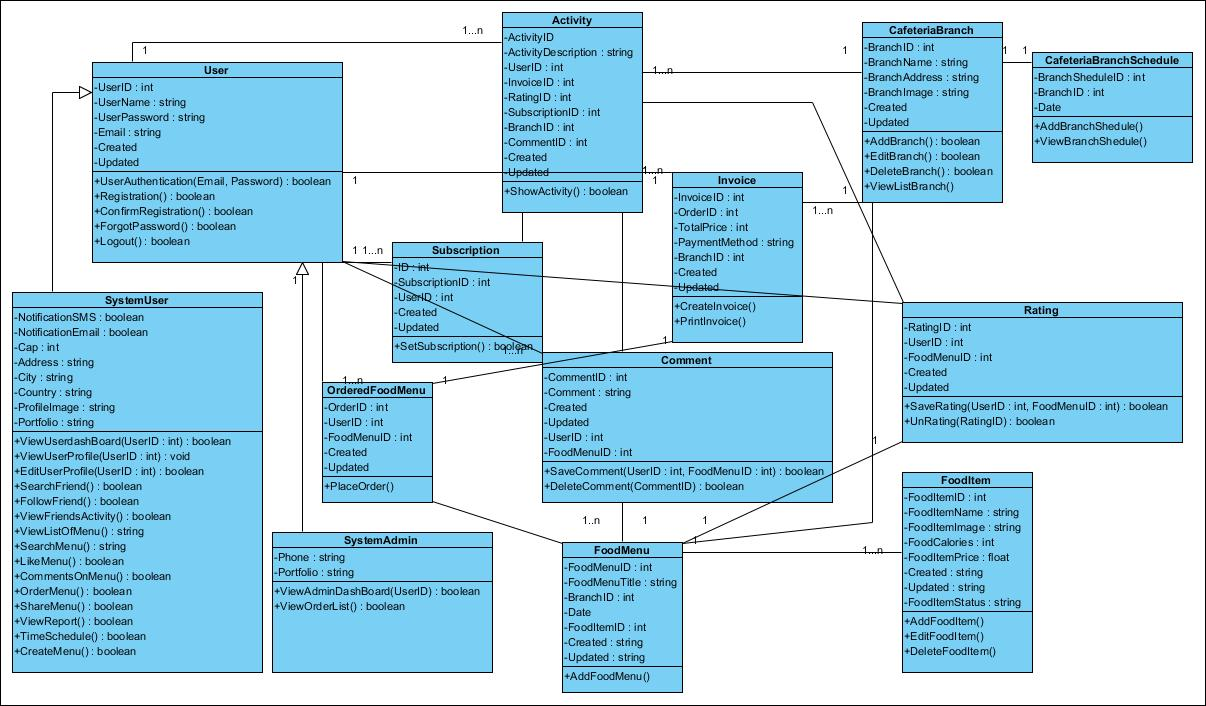
\includegraphics[width=9in]{ch3/ClassDiagram/Class}
  \caption{Class Diagram of Smart Cafeteria}
  \label{ClassDiagram}
\end{figure}
\end{landscape}
\textbf{User:} This class contains information about a user in the smart
cafeteria. The user class has a UserID as a primary key which will be unique,
UserName, UserPassword as credential information, Email address and created and
updated properties. This User class also has some functionality
UserAuthentication which will take arguments as Email and Password,
Registration, ConfirmRegistration, ForgotPassword and Logout. The user class is
associated with Activity, Subscriptions, Comments, Rating and OrderedFoodMenu
classes.

\textbf{System User:}The class System User will be inherited from User class
which means all properties and methods from User class will be included into
System User class. This class also contains some attributes such as
NotificationSMS that is a flag which gives notification users through SMS,
NotificationEmail that also gives notifications users through email, Cap,
Address, City, Country; and created and updated properties. This class also has
some functionalities such as ViewUserDashboard, ViewUserProfile,
EditUserProfile, SearchFriend, FollowFriends, Viewfriendsactivity,
ViewListofMenu, SearchMenu, Likemenu, CommentOnMenu, OrderMenu, ShareMenu,
ViewReport, TimeSchedule, CreateMenu.

\textbf{System Administrator:}The System User class also will be inherited from
User class; means all properties and methods from user class will be included
into system admin class. This class also contains some attributes such as phone
and portfolio. This class contains some functionalities such as
ViewAdminDashboard, ViewListofOrder.

\textbf{Food Item:} Food Item class has FoodItemID, FoodItemName, FoodItemImage,
FoodCalories, FoodItemPrice, FoodItemStatus, cretaed and updated attributes.
This class contains AddFoodItem, EditFoodItem and DeleteFoodtem methods. This
class is associated with FoodMenu and FoodItemID is the foreign key of FoodMenu
class.

\textbf{Food Menu:} Food Menu class contains FoodMenuID, FoodMenuTitle,
BranchID, FoodItemID, cretaed and updated properties.
This class has a method named AddFoodMenu and is associated with Comments,
Rating, FoodItem and OrderFoodMenu.

\textbf{Oder Food Menu:} The OrderedFoodMenu class contains OrderID, UserID,
FoodMenuID, cretaed and updated properties and OrderPlace function. This class
is associated with FoodMenu, Invoice and User classes.

\textbf{Invoice:} The Invoice class contains InvoiceID, OrderID, TotalPrice,
PaymentMethod, BranchID , cretaed and updated attributes. This class also has
CreateInvoice and PrintInvoice methods and associated with Activity.


\textbf{Comment:} Class Comment contains CommentID, Comment, UserID,
FoodMenuID, cretaed and updated properties and SaveComment and DeleteComment
methods. This class is associated with User and FoodMenu classes.

\textbf{Rating:} The class Rating contains RatingID, UserID, FoodMenuID,
cretaed and updated properties and SaveRating and UnRating methods. This class
is associated with User and FoodMenu classes. This class is associated with User
and FoodMenu classes.

\textbf{Subscription:} The class Subscription contains ID, SubscriptionID,
UserID, cretaed and updated properties and Subscription method. This class is
associated with User and Activity classes.

\textbf{Activity:} The class Activity has ActivityID, ActivityDescription,
UserID, InvoiceID, CommentID, RatingID, SubscriptionID, BranchID, cretaed and
updated properties and ShowActivity method. This class is associated with User,
Invoice, Comment, Rating, Subscription and Branch classes.


\textbf{CafeteriaBranch:} The class  CafeteriaBranch contains BranchID,
BranchName, BranchAddress, BranchImage, cretaed and updated properties and
AddBranch, EditBranch, DeleteBranch and ViewListBranch methods. The class
Cafeteriabranch is associated with Invoice, Activity and CafeteriaBranchShedule
classes.

\textbf{CafeteriaBranchSchedule:} The class CafeteiraBranchSchedule contains
BranchScheduleID, BranchID and Date properties and AddBranchSchedule,
ViewBranchSchedule methods. This class is associated with CafeteriaBranch class.


\subsection{Activity Diagram}
\label{subsec:activity}
Activity diagram \cite{UMLActivityDiagram} describes dynamic aspects of any system and
basically represents the flow of activity form one to another activity. The
activity could be described as an operation of the system and this diagram
captures the dynamic behavior of the system. So it is important to visualize
dynamic nature of a system. In this analysis, I have found some activity diagram
of Smart Cafeteria system and shown in figure[\ref{SystemUserActivityDiagram},
\ref{AdministratorActivityDiagram}, \ref{SystemActivityDiagram},
\ref{PointofSaleActivity}] and described step by step.

\subsubsection{System User} When a user browses the system, he or she can
navigate to search food menu, see time schedule, see today's top menu into the
slideshow and browse today's food menus. Users also can register in the system
and login into the system.  After successfully login into the system, user as a
registered user could navigate previous basic activities search food menu, see
time schedule as well as could browse User Dashboard from where user could
search friends, follow friends, see friend's activities, see dieting reports,
create food menu from foods, comment on food menus, like food menus, share food
menus and order food menus. Users also could change profiles and logout from
this stage.
The system will do some activities alone with user such as suggest daily
different food menus for different users based on users interest and previous
food consumed and dieting history. System will also save registration
information of user after registration and check account credential before login
action. After all actions, system saves preferences as well. In the figure
\ref{SystemUserActivityDiagram}, shows the activity of users as simultaneously
with system.

\begin{figure}[h!t]
    \centering
      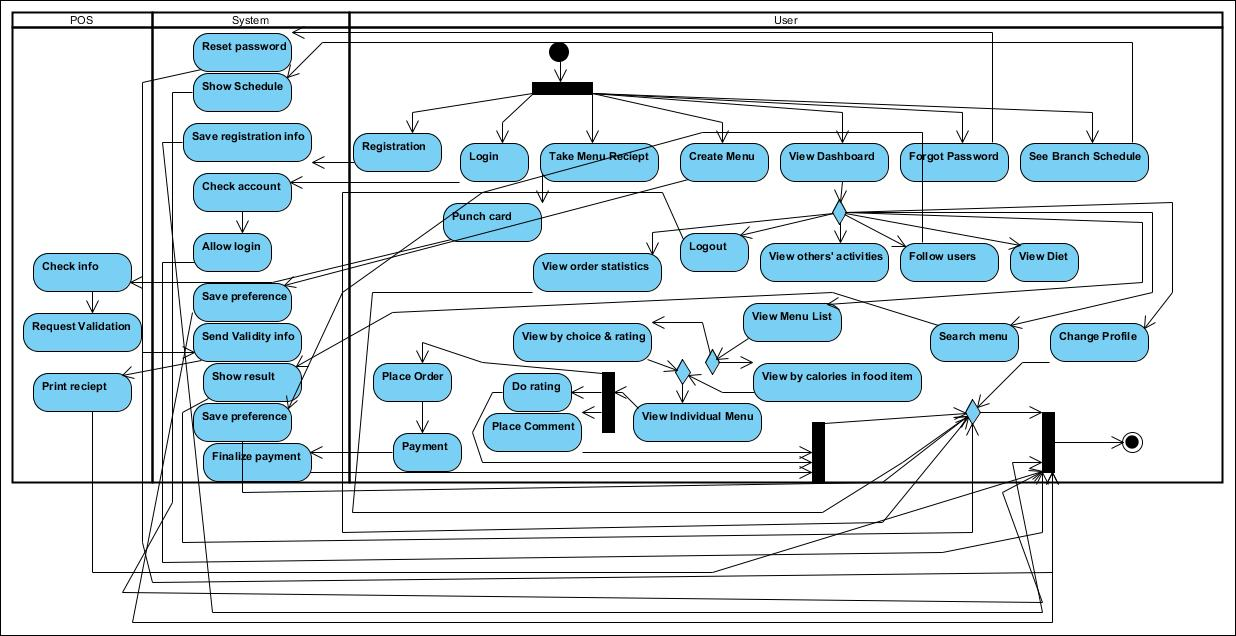
\includegraphics[width=6in,height=6in]{ch3/ActivityDiagram/SystemUser}
  \caption{System User Activity Diagram of Smart Cafeteria}
  \label{SystemUserActivityDiagram}
\end{figure}

\subsubsection{System Administrator} System administrator has some flow of activity
after login into the system using administrator panel. System Administrator
could view order pending from user's order and can confirm the order; and
search report and system show report as well. From dashboard, system
administrator can do different activity; manage food item, food menu, view order
statistics and manage order statistics into different request such as view order
by day, view order by month or view order by menu; and system response as well
in the every activity.In the figure \ref{AdministratorActivityDiagram}, shows
the activity of System Administrator.

\begin{figure}[h!t]
    \centering
      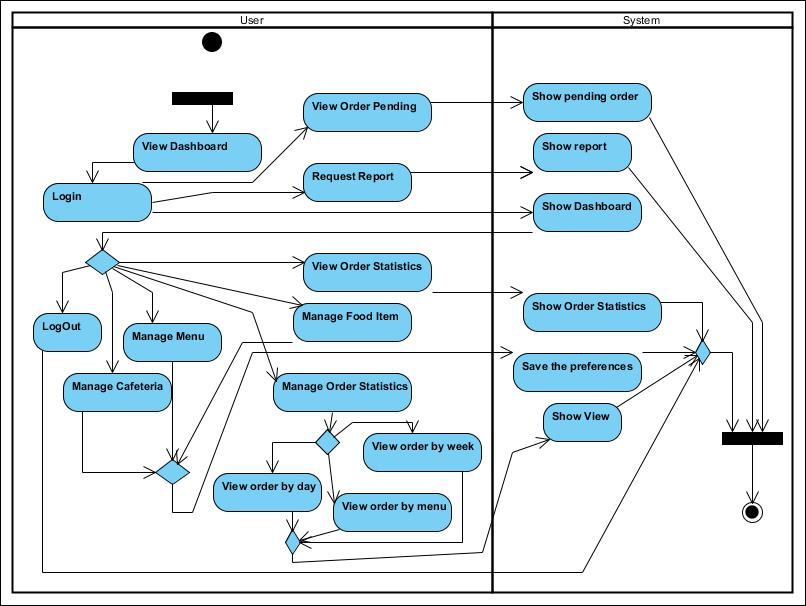
\includegraphics[width=5.5in]{ch3/ActivityDiagram/SysAdmin}
  \caption{System Administrator Activity Diagram}
  \label{AdministratorActivityDiagram}
\end{figure}

\subsubsection{System} In the system, there are some very important activities such
as receive order confirmation from users, generate diet reports, create food
suggestions, generate different kinds of notifications and send to users. The
system looks after both type of user's; system users and system administrators,
session and credentials as well. In the figure \ref{SystemActivityDiagram} shows
the activity of System.
\begin{figure}[h!t]
    \centering
      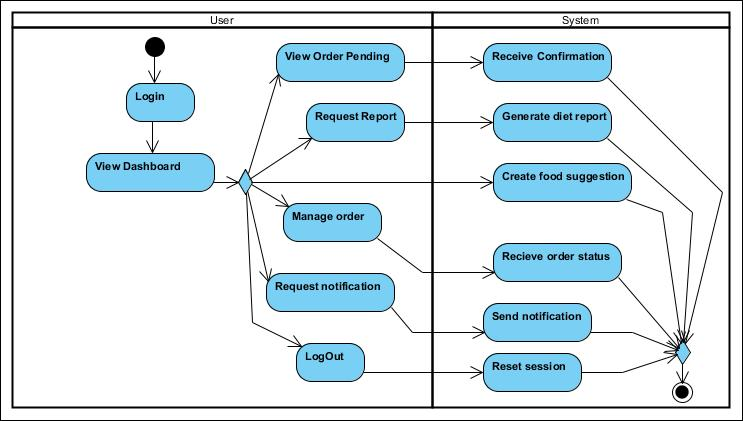
\includegraphics[width=5.5in]{ch3/ActivityDiagram/SysApp}
  \caption{System Activity Diagram}
  \label{SystemActivityDiagram}
\end{figure}

\subsubsection{Point of Sale} After confirmation of order, users punch card into
POS terminal and those POS terminations are responsible to print order receipt
for users and send a notification to the system application to update that the
food menu is being served. In the figure \ref{PointofSaleActivity} shows the
activity of Point of Sale.

\begin{figure}[h!t]
    \centering
      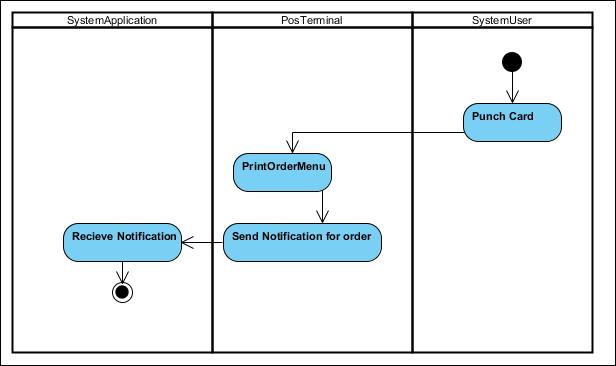
\includegraphics[width=5.5in]{ch3/ActivityDiagram/POS}
  \caption{Point of Sale Activity Diagram}
  \label{PointofSaleActivity}
\end{figure}

\clearpage
\newpage
%\thispagestyle{empty}
\mbox{}
%\enlargethispage*{1000pt}

\chapter{Smart Cafeteria Design}
\label{chap:DesignofSmartCafeteria}
In this chapter, I have discussed the design of ``Smart Cafeteria''. In first
[\ref{sec:CAD}] and second [\ref{sec:SOA}] section, conceptual architecture and
design and service oriented architecture (SOA) was discussed respectively. These
are the top level architecture and design of the system. In the next section
[\ref{sec:PrototypeSC}] prototype of ``Smart Cafeteria'' is discussed; a mid
fidelity prototype of all functionalities of the system; some of them was
covered in desktop prototype [\ref{subsec:prototypefordesktop}] and the rest was
covered in mobile prototype [\ref{subsec:PrototypeforMobile}]. And the final
section [\ref{sec:keyFeaturesSC}] was discussed about the key features of the
system.

\section{Conceptual Architecture And Design}
\label{sec:CAD}
A conceptual architecture~\cite{Zamg} describes essential and top level features
of a system and identifies the main processes and their flows taking place in
the system. It provides a definition of the phenomenon in terms of features
recognizable by analysis and observations; and describes the abstract life cycle
of the system.

Conceptual design~\cite{MicrosoftCorporation2003} is the process of gathering,
analyzing, and prioritizing business and user perspectives of the problem and
the solution, and then creating a high-level representation of the solution.
Conceptual design should follow three principle steps in any system
development life cycle; research, analysis and optimization by system designer.


In the figure \ref{ConceptualArchitecture_top_level} a top level architecture of
``Smart Cafeteria'' application is shown.
The mobile appplication users interact with the system through interface of the
mobile application and desktop users interact with the system through browser.
\begin{figure}[h!t]
    \centering
      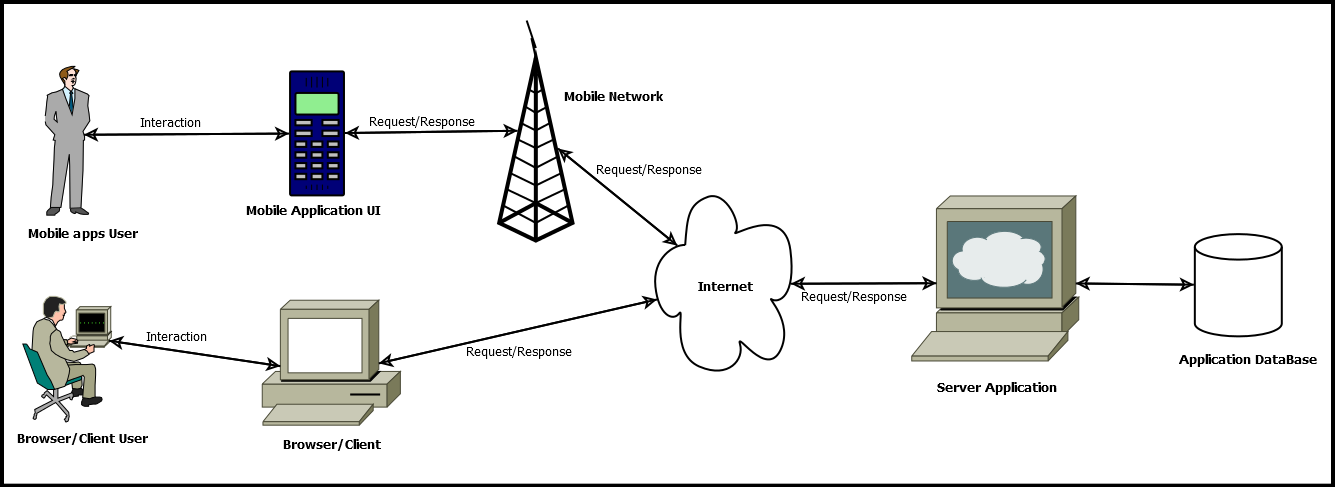
\includegraphics[width=5.5in]{ch4/SOA/ConceptualArchitecture}
  \caption{Conceptual Architecture of Smart Cafeteria[Top Level]}
  \label{ConceptualArchitecture_top_level}
\end{figure}

\begin{figure}[h!t]
    \centering
      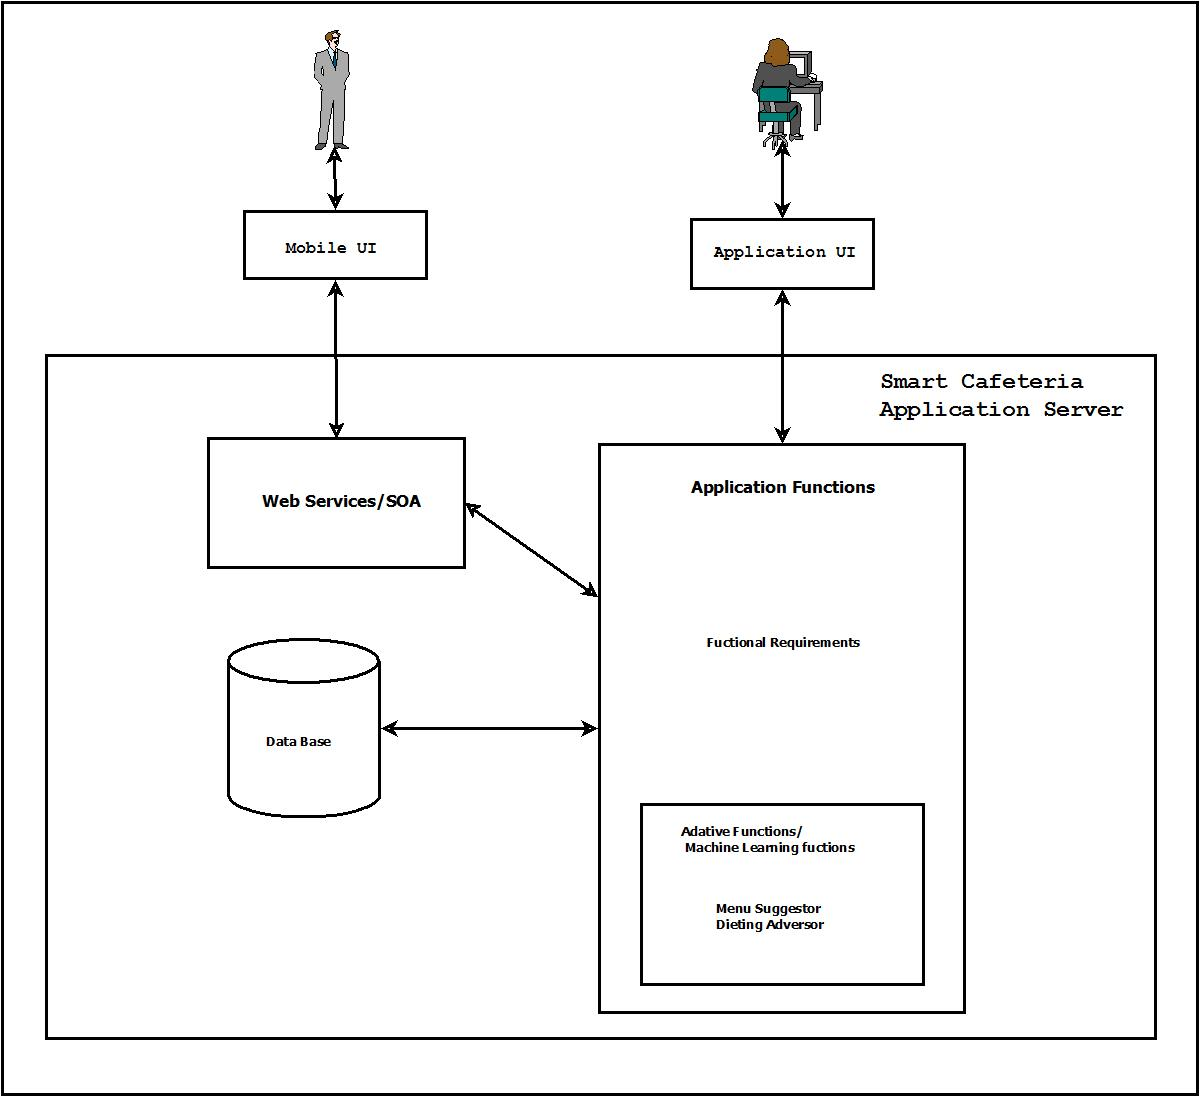
\includegraphics[width=5.5in,height=5in]{ch4/SOA/ConceptualArchitecture_new}
  \caption{Conceptual Design of Smart Cafeteria[Server Level]}
  \label{ConceptualArchitecture_server_level}
\end{figure}
In the figure~\ref{ConceptualArchitecture_server_level}, server level
conceptual design has been shown where application fuctionalities and
web services/SOA intergrates together to support mobile apps as well as desktop
application. Most of the process of conceptual design has been discussed in
Chapter~\ref{chap:AnalysisofSmartCafeteria}.

Within the application architecture, some fuctions of our application are
adaptive which support adaptivity features such as menu suggestor, dieting
advisor. Since smart cafeteria appplication will also support as a mobile
application, Service Oriented Architecture(SOA) is very important to implement
mobile application functionalities which is discussed in section~\ref{sec:SOA}.


\section{Service Oriented Architecture(SOA)}
\label{sec:SOA}
In recent years, the information technology has moved towards service oriented
architectures, especially in mobile computing and distributed computing. Since
the number of different clients such as mobile applications, tablet applications
are increasing rapidly; an emerging need of using SOA and Web services are also
increasing to support those applications. The Service Oriented Architecture
(SOA) recognizes and tries to construct a distributed, dynamic, flexible, and
reconfigurable service system over Internet~\cite{Aydin2007}.

The key feature of service orientation architecture is loose coupling that is
using resources only published but not accessable directly implementation behind
application. So the change in implementation by the service provider should not
affect the service consumer, for instance, weather service consumer and provider
have the same technologies for the implementation application, interface. SOA is
itself stateless which means it does not depend on the state of other services
and also support reuse of software components because of loose coupling. The key
component in SOA is web services that are well defined set of
actions~\cite{Linthicum2004,Sahin2008}.

\citet{Akinci2004} discussed about properties of web services; firstly,
web services are for application-to-application communication. Secondly, web
services are accessed over Internet. And finally, web services are XML based
open standards, such as WSDL, SOAP to support interoperable machine to machine
interaction over a network.

Richer UI could be the client side web service technologies such as Java
Applets, Flash, Flex, Silverlight, iOS application, Android Application, HTML5
that must has quick response. Services Layer are  Stateless Services and most of
cases XML, REST or JSON that will get from Object oriented program function such
as java, Ruby, Python, etc.

The following figure[~\ref{SOAArchitecture}] shows Service Oriented Architecture
of smart cafeteria.

\begin{figure}[h!t]
    \centering
      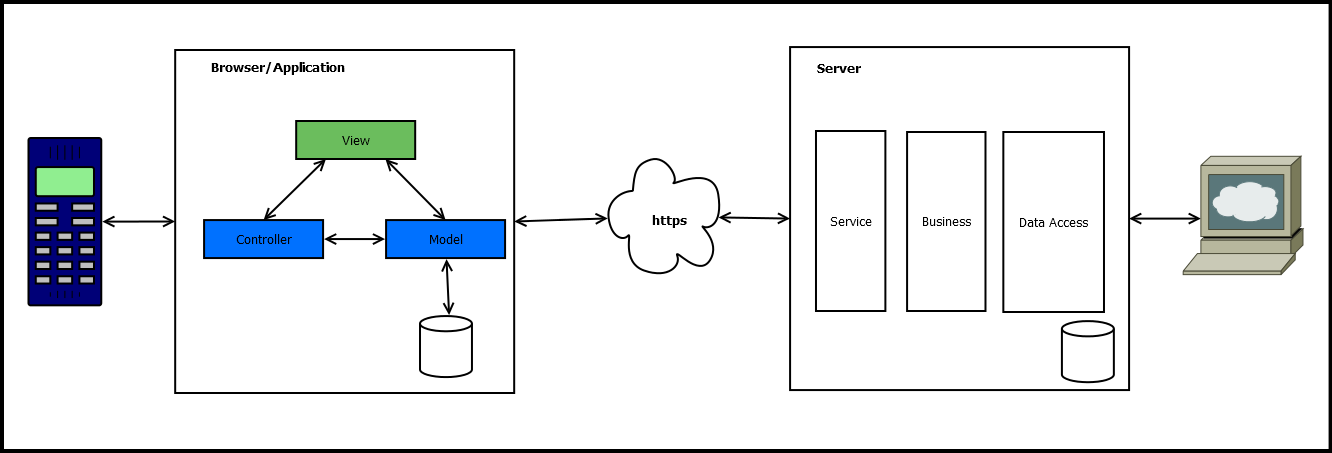
\includegraphics[width=5.5in]{ch4/SOA/SOAArchitecture}
  \caption{SOA Architecture of Smart Cafeteria}
  \label{SOAArchitecture}
\end{figure}


\section{Prototype of Smart Cafeteria}
\label{sec:PrototypeSC}
Prototyping~\cite{Mads2010,Greenberg}, the process of developing prototypes, is
a method used by designers to get feedback from users about future designs.
Prototypes are experimental and incomplete designs of system which are cheap;
can be developed quickly and it is an essential part of iterative user-centered
design.

The main purpose of prototyping is to involve the users in testing design ideas
and get their feedback in the early stage of development, to reduce cost and
save time. It provides an efficient and effective way to optimize interfaces
through interactive discussion and testing. The prototypes can be changed
multiple time until a stable version of user interface that has been
accomplished with efforts both from designers and users.

Prototyping can be divided into three categories; low-fidelity prototyping,
medium-fidelity prototyping and high-fidelity prototyping. In some literature,
it is simply classified as low-fidelity prototyping and high-fidelity
prototyping, where low-fidelity prototyping is mainly about paper-based mock-up
such as Sketches, Storyboard and high-fidelity is mainly about computer-based
simulation. High-fidelity prototypes are fully interactive, simulating most of
the functionality of the final product whereas medium-fidelity prototypes are
computer-based simulation too but it simulates the system interaction and
functionality partially; not all features of the intended system.


I have designed and demonstrate most of the functionalities and requirements
which I have gathered in previous chapter~\ref{chap:AnalysisofSmartCafeteria}.
According to structural diagram (Class Diagram \ref{subsec:classdiagram}) and
dynamic diagram (Activity Diagram \ref{subsec:activity}) in UML 2, I have come
to a stage from where I have proposed a medium fidelity prototype which meets
and shows initial visualization of most fundamental functionalities and
requirements.

To demonstrate and discuss full design template, I will discuss some
functionalities in desktop prototype section \ref{subsec:prototypefordesktop}
and rest of them will be discussed in mobile prototype section
\ref{subsec:PrototypeforMobile}.

\subsection{Desktop Prototype}
\label{subsec:prototypefordesktop}
In this thesis work, I have designed a medium fidelity prototype of smart
cafeteria.


The prototype of smart cafeteria has been designed by
HTML5\footnote{\href{http://www.w3.org/TR/html51/}{HTML 5}},
CSS3\footnote{\href{http://www.w3.org/TR/CSS/}{Cascading Style Sheets (CSS3)}}
and Twitter
Bootstrap\footnote{\href{http://twitter.github.io/bootstrap/}{Twitter
Bootstrap}} jQuery plugins.  To design the template, I have used Eclipse IDE
Juno\footnote{\href{http://twitter.github.io/bootstrap/}{Eclipse IDE}} and run
that on Apache Tomcat server
v7.0\footnote{\href{http://tomcat.apache.org/}{Apache Tomcat server v7.0}}.


There are two basic main part in the prototype; index \ref{indexpage} which will
come after starting the application or browsing the application and dashboard
\ref{dashboardpage} will be accessible after user logs into the system.

\subsubsection{Index}
\label{indexpage}
In the index page, there are a couple of functionalities; among them search food
menu, signup, login, todays hot food menu slider and today's all food menus are
most common. Using user information such as user name and password, user could
go into user dashboard page. There are two steps in signup activity; the first
step is for basic information of user and the last step will ask user's
additional information which will help to calculate user's dieting information
and suggesting food menu by some adaptive mechanism such as machine learning
methods. The functionality of user's password recovery also exists there. There
exists two navigation shortcuts link such as search more menu and time schedule
of cafeteria and branches. This page also contains a list of today's food menu
supported by pagination functionality that are divided into three subcategory;
full menu, half menu and snacks. In full menu, there are three types of menu
courses such as first course (pasta or rice and sauce), second course (fish or
meat and vegetable soup) and desert. Since the proposed system would support as
dynamic content management so we should not concentrate about number of foods
and food menus. In the figure \ref{PLindex}, demonstrate a medium fidelity
prototype of index page of Smart cafeteria system.

\begin{figure}[h!t]
    \centering
    \fbox{
      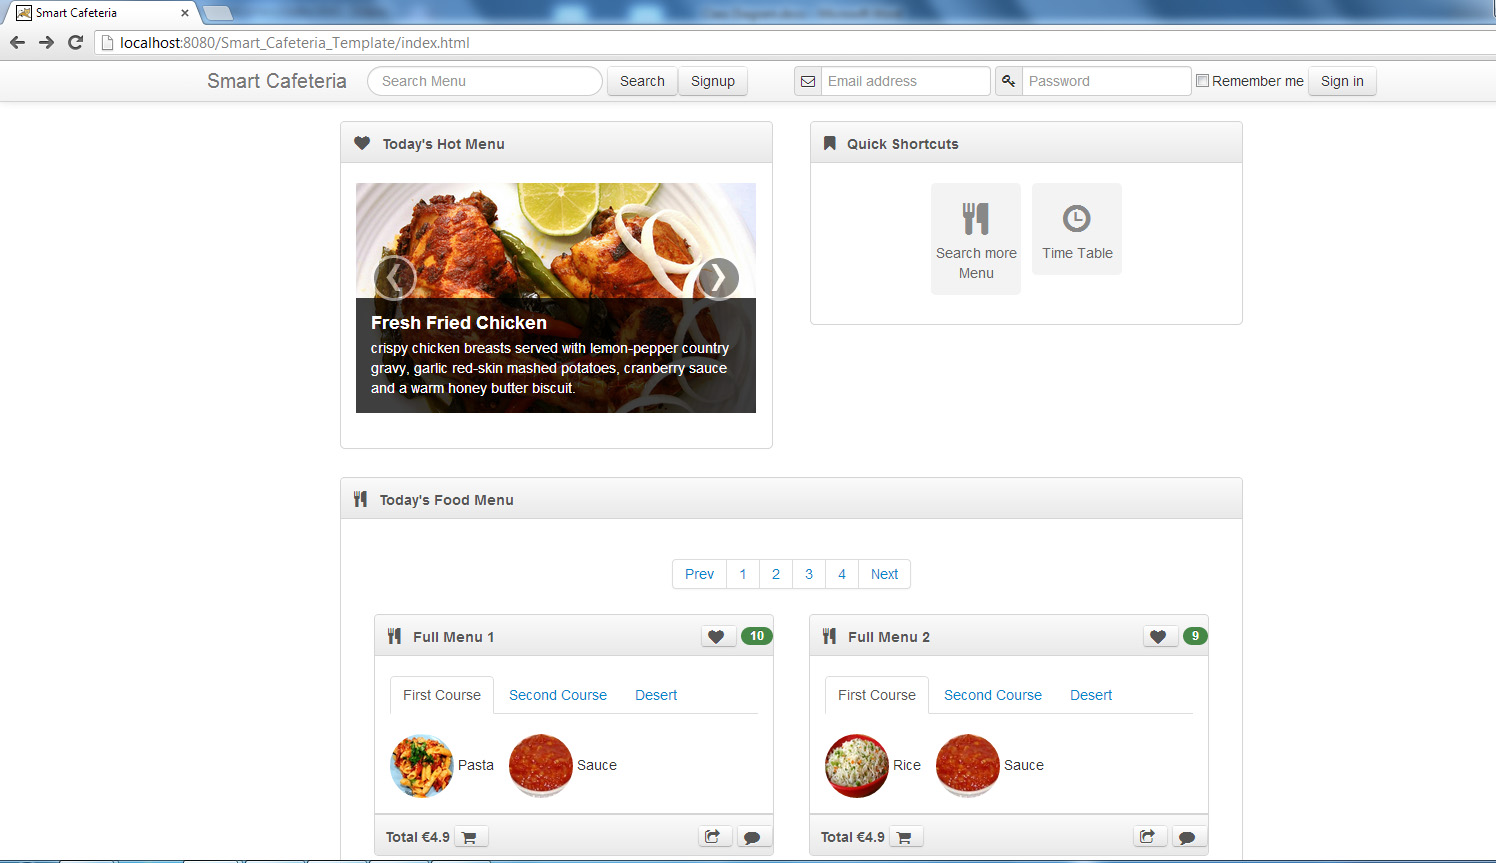
\includegraphics[width=5.5in]{ch4/Prototype/Laptop/index}
      }
  \caption{Index of Smart Cafeteria}
  \label{PLindex}
\end{figure}

\subsubsection{Dashboard}
\label{dashboardpage}
 This is the most important page in the system where credentials are required to
 get access. In this page, there are two sides; upper side of the page
 [Figure~\ref{PLdashboard}] consist navigation shortcuts and a short report of
  food consumption by user and lower side of the page
  [Figure~\ref{PLfoodmenusuggestion}] consists
 suggested food menu by the system using adaptive mechanism (Machine learning
 approach). The navigation shortcuts [Figure~\ref{PLdashboard}] consists
 different functionalities such as search menu, search friends, see follower,
 friend's activities, show dieting reports, create custom menu, show time table
 and branches.
 
\begin{figure}[h!t]
    \centering
      \fbox{
      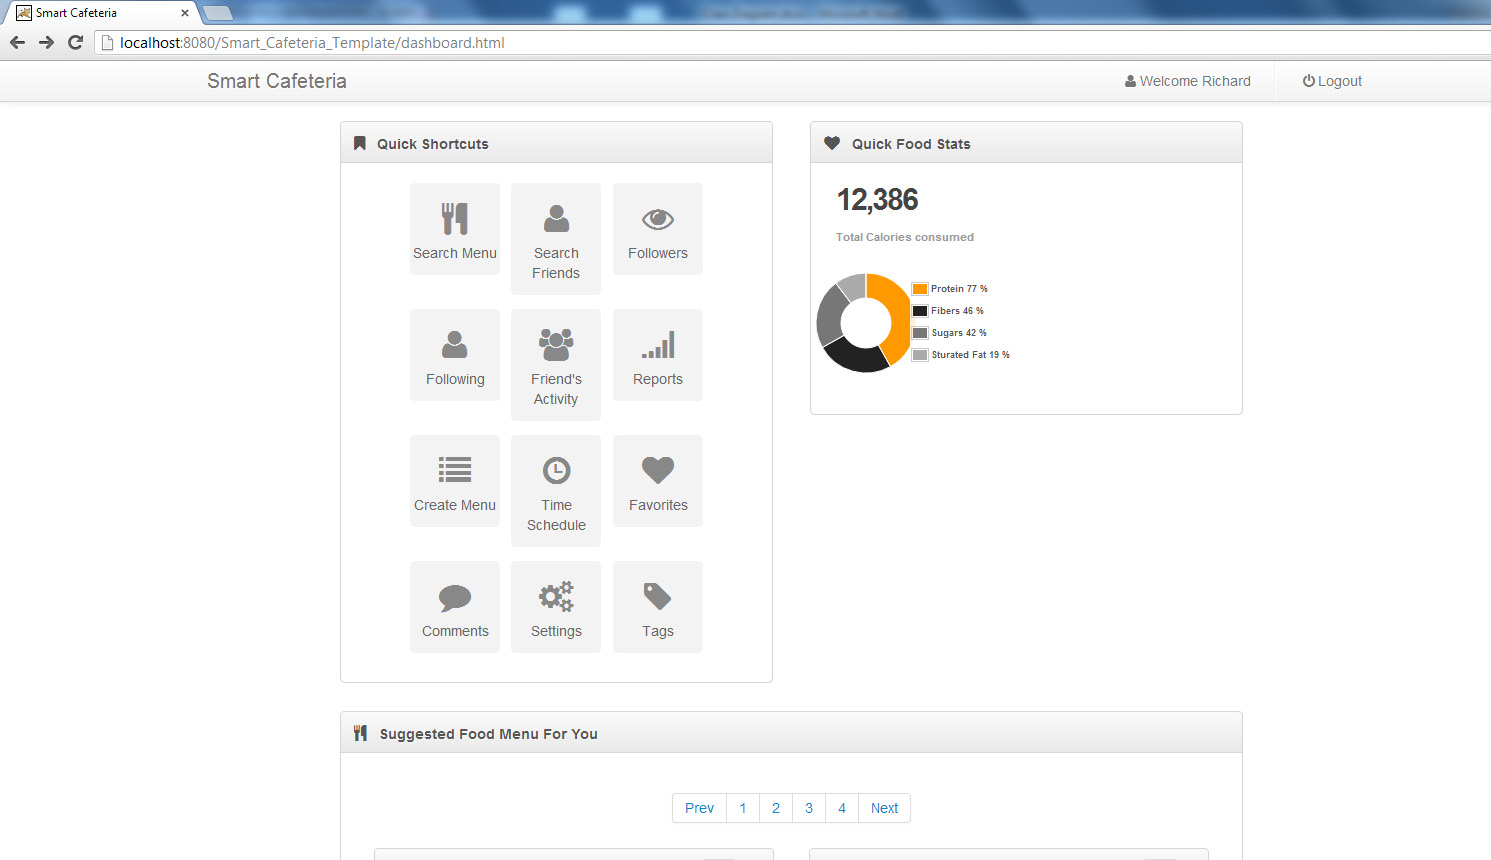
\includegraphics[width=5.5in,height=3.4in]{ch4/Prototype/Laptop/dashboard}
      }
  \caption{Dashboard of Smart Cafeteria [Navigation]}
  \label{PLdashboard}
\end{figure}

\begin{figure}[h!t]
    \centering
      \fbox{
      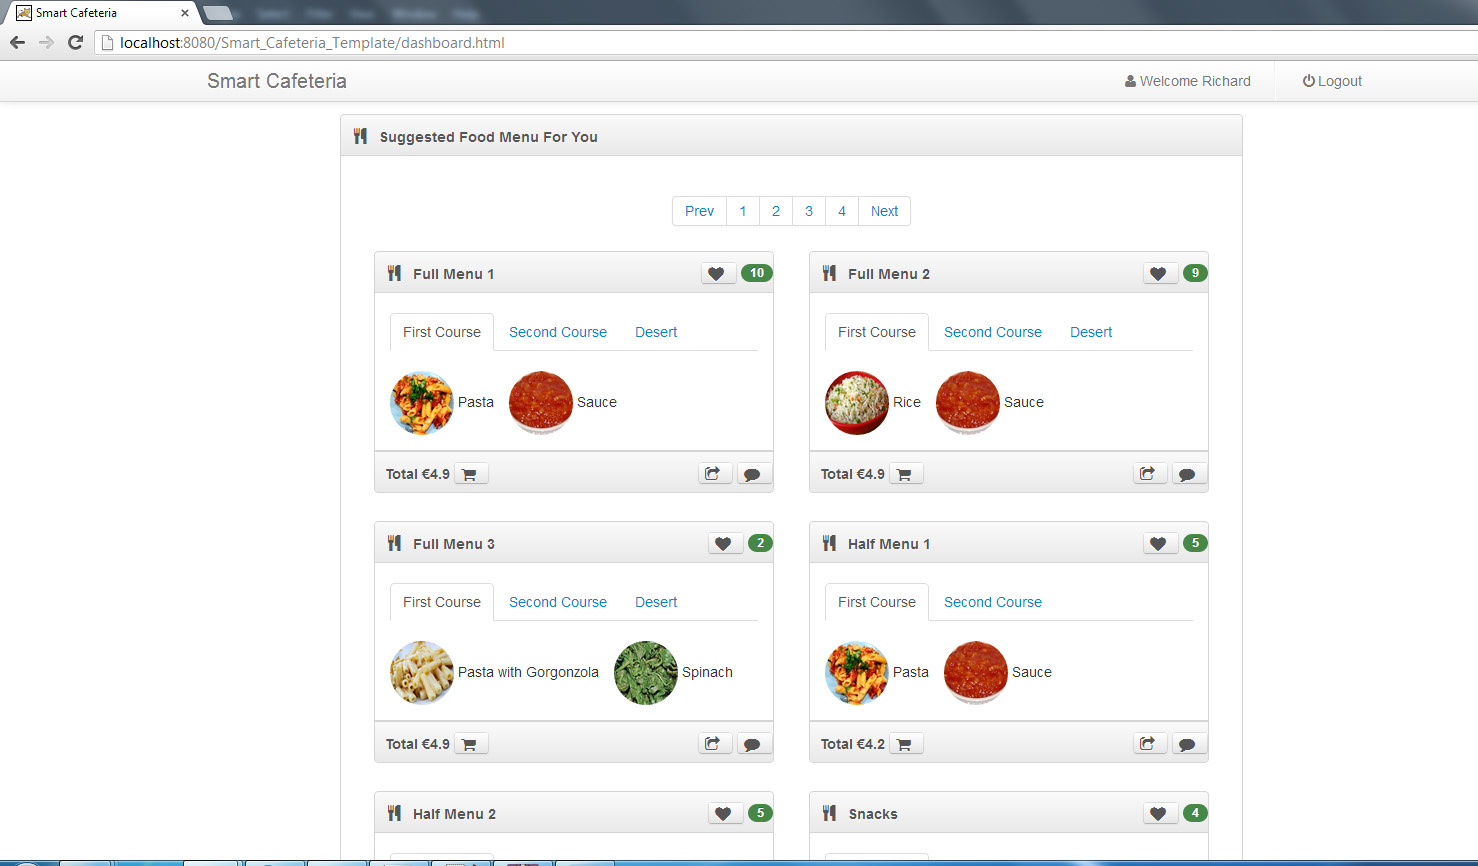
\includegraphics[width=5.5in,,height=3.4in]{ch4/Prototype/Laptop/foodmenusuggestion}
      }
  \caption{Dashboard of Smart Cafeteria [Today's \& Suggested food menu]}
  \label{PLfoodmenusuggestion}
\end{figure}

\newpage
\subsection{Mobile Prototype}
\label{subsec:PrototypeforMobile}
The prototype of smart cafeteria for mobile plateform was designed with HTML5,
CSS3 and Twitter Bootstrap jQuery plugins. To design and demonstrate the
template, I have used phonegap\footnote{\href{http://phonegap.com/}{Phonegap}}
tools for implemention as it supports most of mobile OS such as android, iOS.
I have described some functionalities in the previous
section~\ref{subsec:prototypefordesktop} and the rest of the functionalities of
smart cafeteria I will be demonstrated in this section.

\subsubsection{Index}
\label{Indexpagemobile}
The index page contains search food menu, signup, login, today's hot food menu
slider and today's all food menus offered by cafeteria. In the
figure~\ref{fig:PMInstalledIndex}, left shows installed smart cafeteria apps and
the right shows index page of smart cafeteria.

\begin{figure}[h]
\centering
      \fbox{
\begin{subfigure}[b]{.5\textwidth}
  \centering
    \fbox{
  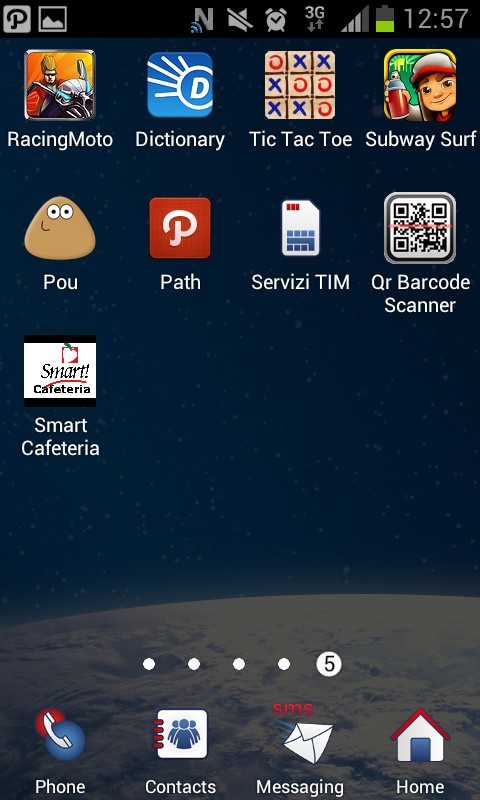
\includegraphics[width=0.9\textwidth]{ch4/Prototype/Mobile/mobile-installed.png}
  }
\end{subfigure}%
\begin{subfigure}[b]{.5\textwidth}
  \centering
  \fbox{
  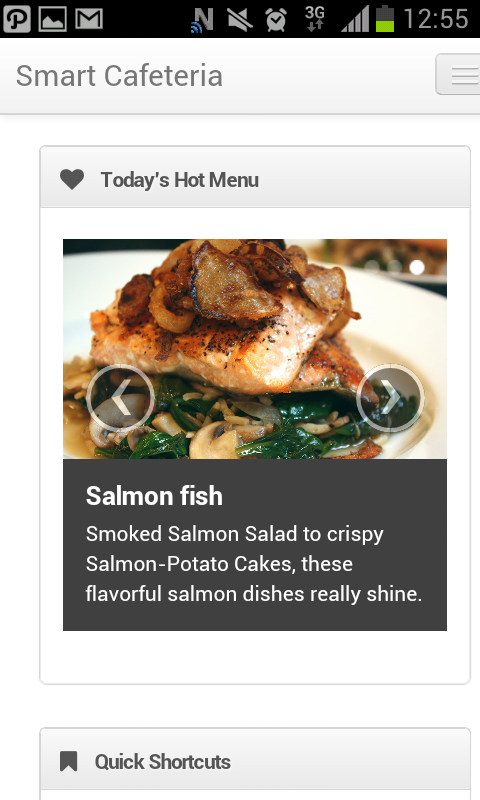
\includegraphics[width=0.9\linewidth]{ch4/Prototype/Mobile/mobile-index.png}
  }
\end{subfigure}
}
\caption{Installed Smart Cafeteria Apps(Left). Index page of Smart Cafeteria (Right).}
\label{fig:PMInstalledIndex}
\end{figure}
\newpage

\subsubsection{User Registration}
\label{UserRegistration}
The registration has two steps; step one needs the basic information of users
such as User Name, Email, password which is shown in left of the figure
\ref{fig:PMUserRegistration} and on the right of the figure
\ref{fig:PMUserRegistration} step two which asks users' physical
information which will help to calculate dieting report and suggest appropriate
food menu is shown.
\begin{figure}[h]
\centering
  \fbox{
\begin{subfigure}[b]{.5\textwidth}
  \centering
   \fbox{
  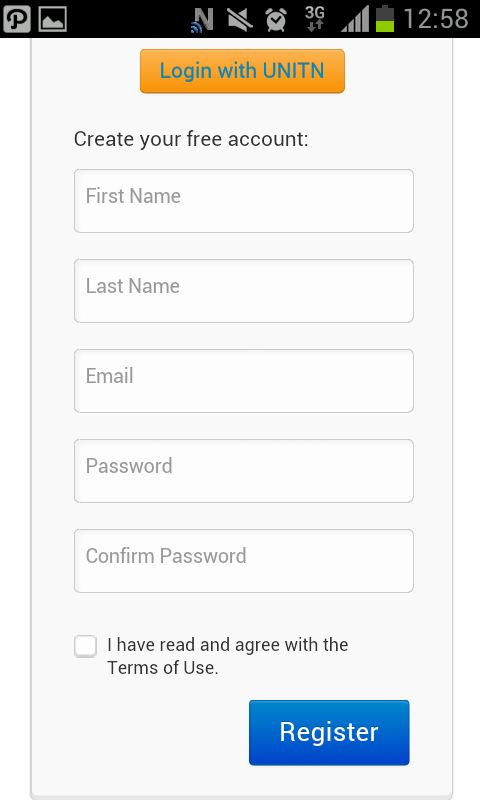
\includegraphics[width=0.9\textwidth]{ch4/Prototype/Mobile/mobile-registration-step1}
  }
\end{subfigure}%
\begin{subfigure}[b]{.5\textwidth}
  \centering
   \fbox{
  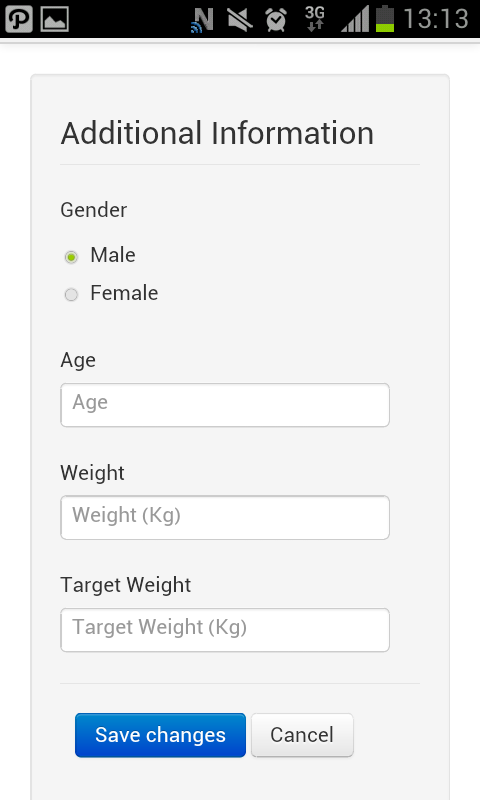
\includegraphics[width=0.9\linewidth]{ch4/Prototype/Mobile/mobile-registration-step2}
  }
\end{subfigure}
}
\caption{User Registration step one of smart cafeteria (Left). User Registration step two of smart cafeteria (Right).}
\label{fig:PMUserRegistration}
\end{figure}


\subsubsection{User Login and Password Recovery}
\label{UserLoginandPasswordRecovery}
To use full functionalities of the system such as order food menu, follow
friends, share lunch item with friends; it is very important to login into the
system. Since sometimes it is essential to recover password in any system,
password recovery also an important function in the smart cafeteria. In the left
of the figure~\ref{fig:PMUserLogin} shows user Login of smart cafeteria and in
the right of the figure~\ref{fig:PMUserLogin} shows user Password Recovery of
smart cafeteria.

\begin{figure}[h]
\centering
  \fbox{
\begin{subfigure}[b]{.5\textwidth}
  \centering
        \fbox{
  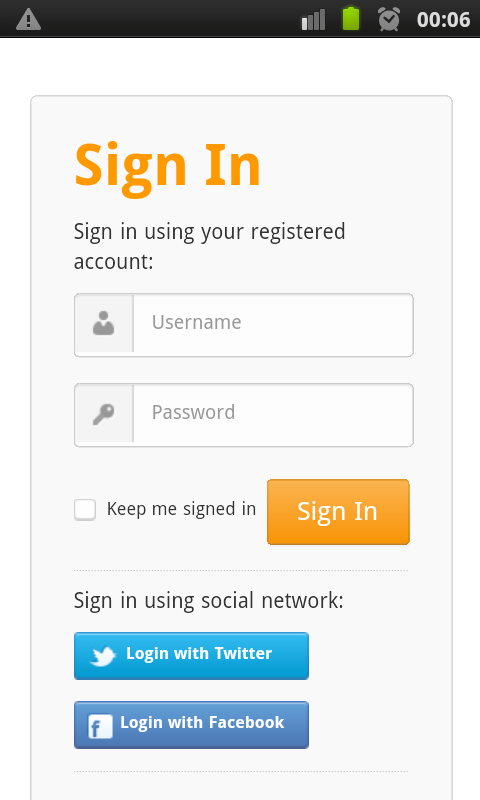
\includegraphics[width=0.9\textwidth]{ch4/Prototype/Mobile/login}
  }
\end{subfigure}%
\begin{subfigure}[b]{.5\textwidth}
  \centering
        \fbox{
  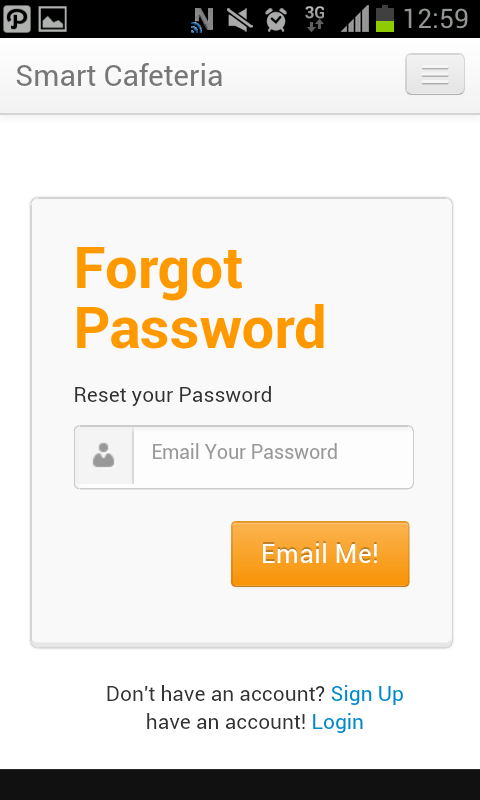
\includegraphics[width=0.9\linewidth]{ch4/Prototype/Mobile/forgotpassword}
  }
\end{subfigure}
}
\caption{User Login of smart cafeteria (Left). User Password Recovery of smart cafeteria (Right).}
\label{fig:PMUserLogin}
\end{figure}

\subsubsection{Generate dieting report}
\label{Generatedietingreport}
Since the system will store the basic information of users as well as their
physical information; using these information through some machine learning
approach, system will generate dieting report, menu suggestion as an adaptive
system. In the left of the figure~\ref{fig:PMReport} shows users dieting report
of smart cafeteria and in the right of the figure~\ref{fig:PMReport} shows
Nutrition Suggestion for user of smart cafeteria.

\begin{figure}[h]
\centering
      \fbox{
\begin{subfigure}[b]{.5\textwidth}
  \centering
        \fbox{
  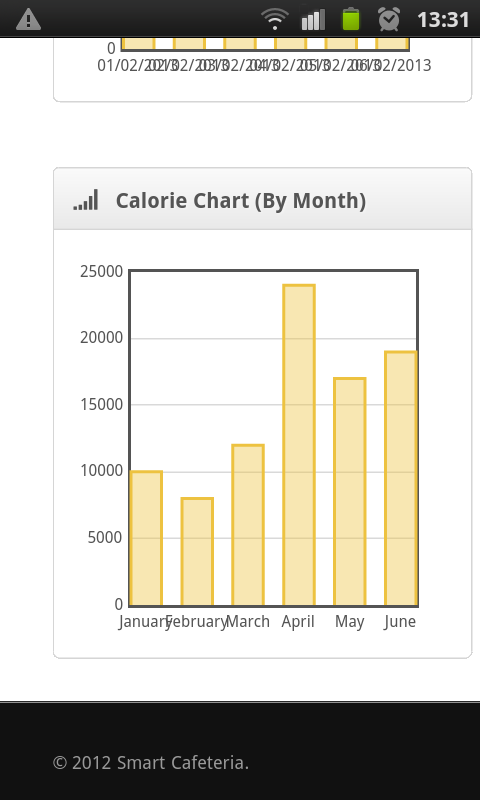
\includegraphics[width=0.9\textwidth]{ch4/Prototype/Mobile/report}
  }
\end{subfigure}%
\begin{subfigure}[b]{.5\textwidth}
  \centering
        \fbox{
  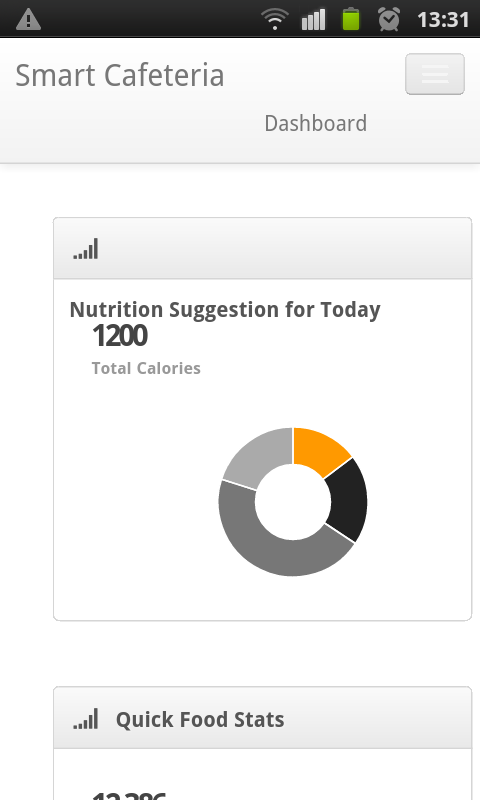
\includegraphics[width=0.9\linewidth]{ch4/Prototype/Mobile/suggestion}
  }
\end{subfigure}
}
\caption{Dieting Report for User of smart cafeteria (Left). Nutrition Suggestion of smart cafeteria (Right).}
\label{fig:PMReport}
\end{figure}
\newpage

\subsubsection{Collaborative and Sharing Activities}
\label{Searchfollowingfriends}
Since Smart cafeteria support collaborative activities, the design template
consists those functionalities: search friends, follow friends and sharing their
activities which will make the system more interactive and usable in user
prospective. In the left of the figure~\ref{fig:PMUserFollow} shows following
friends functionality of smart cafeteria and in the right of the
figure~\ref{fig:PMUserFollow} shows friends activity of smart cafeteria.

\begin{figure}[h]
\centering
      \fbox{
\begin{subfigure}[b]{.5\textwidth}
  \centering
        \fbox{
  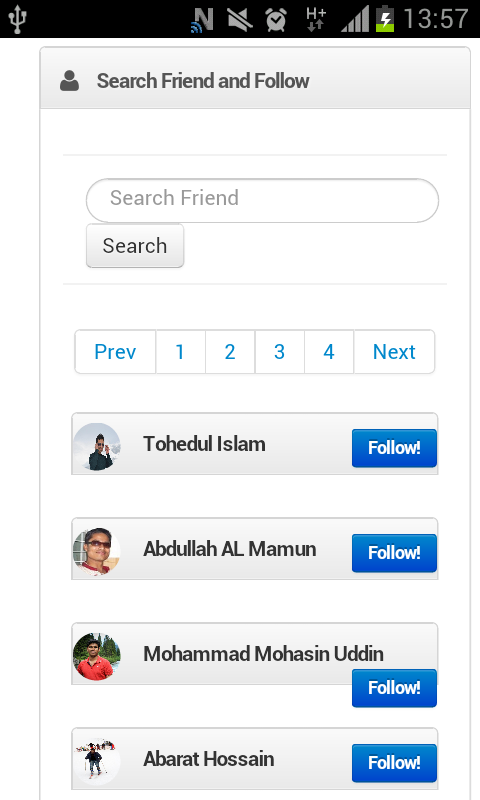
\includegraphics[width=0.9\textwidth]{ch4/Prototype/Mobile/following}
  }
\end{subfigure}%
\begin{subfigure}[b]{.5\textwidth}
  \centering
        \fbox{
  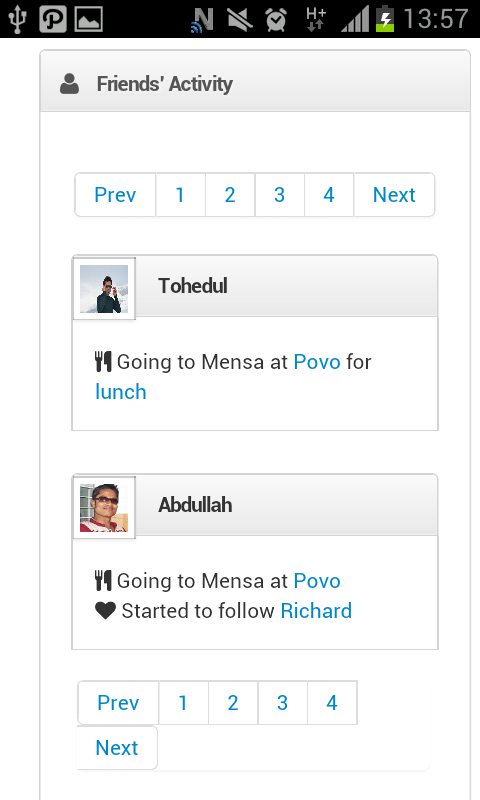
\includegraphics[width=0.9\linewidth]{ch4/Prototype/Mobile/friendsactivity}
  }
\end{subfigure}
}
\caption{: Following Friends for User of smart cafeteria (Left). Friends activity of smart cafeteria (Right).}
\label{fig:PMUserFollow}
\end{figure}
\newpage

\section{Key Features of Smart Cafeteria}
\label{sec:keyFeaturesSC}
There are three key feature in proposed smart cafeteria system which will
support this system's analysis as a research work. The features are listed and
describing bellow:

\subsection{Online Cafeteria services}
The application will provide online cafeteria services where user could search
food menu, order online food menu, pay online that will support
university's cafeteria queue skipper; namely users could browse and choose their
food menu before entering cafeteria. Thus user could easily skip long queue that
seems to be very annoying task in every day lunch time at university. At the same
time, through this application, user could get knowledge about every day food
menu in different branch and acknowledge about time schedule of all branches of
cafeteria. This is very important services now days in university to make life
easy and enjoyable.

\subsection{Adaptive services}
The application will provide online adaptability services such as daily menu
suggestion based on users' previous choice and calorie consumption of the users
in the last couple of weeks. The system will also provide dieting report of
every user which makes the life of the people more comfortable, more enjoyable
and happier. This is very important issue especially for students so these
adaptive services will have a great significance in university life without any
doubt.

\subsection{Social collaboration services}
The application will provide such an environment where user could interact in
social collaboration such as follow friends, share food menu with friends, share
activities of social eating as well as can see friend's activities. These services
will help students to increase collaboration between domestic students with
international students due to exchange food culture, language or psychological
peer supporting.

\subsection{Mobile Interaction}
Now a days, only web 2.0 applications are not sufficient to provide services to
users; a huge number of users want to get the application's services using Smart
phone. People are now used to get portable services to ensure maximum level of
satisfaction and enjoyable experience from application. Since Smart cafeteria
will provide services to university students, so all services and
functionalities of Smart Cafeteria should be supported by mobile apps and tablet
apps. So the plan is to make the application services portable, enjoyable,
usable using smart phone application  to help students.



\clearpage
\newpage
%\thispagestyle{empty}
\mbox{}

\chapter{Usability Evaluation of Smart Cafeteria}
\label{chap:EvaluationSC}
In interactive system design, usability evaluation appears to be very vital
issue in the design life cycle and development process. Sometimes,
usability evaluation is performed in user-centric design at the very
beginning stage with low fidelity prototype such as paper based prototype; or at
requirements gathering stage using focus group and survey questionnaire to get
users' feedback which helps to find out more requirements to make a system
stable; and the modification process continues until the final version of the
product.


The usability evaluation goals of ``Smart Cafeteria" is to test usefulness of
the system, how easy the system to use, Satisfaction, learnability and find out
more requirements to improve the design. To know and figure out best evaluation
methods for ``Smart Cafeteria'', I have studied a couple of article, paper and
book which is discussed here.



\citet{Nielsen2003} define five usability components to assesses how easy user
interfaces are to use. These are Learnability, Efficiency, Memorability, Errors
and Satisfaction.

\citet{Dix2004} defines usability as quality attribute of a system that ensure
the efficiency, effectiveness and satisfaction of specified users to achieve
specified goals in particular environment. They suggested making a distinction
between evaluation by the users at early design stage using focus groups,
survey questionnaires and the evaluation by the designer or a usability expert
at completed system or functional prototype design stage as a cheap and quick
usability assessment. According to their consideration, there are four
approaches for expert analysis: cognitive walkthrough, heuristic evaluation, the
use of models and use of previous work.

In the cognitive walkthrough, the sequence of actions will be performed in order
to accomplish some known task by the users in the system and the principle focus
of the cognitive walkthrough methodology  is to establish how easy a system is
to learn.

Heuristic evaluation, developed by Jakob Nielsen and Rolf Molich, is performed
in design specification stage or early design evaluation stage but could also be
used on prototypes, fully functioning systems.

There are four approaches for user analysis too: empirical or experimental
methods, observational methods, query techniques, and methods that use
physiological monitoring.

Query techniques are a kind of evaluation techniques that is asking the user
about the interface directly and these could be useful in drawing out detail
about the user's view of a system and collect information about user
requirements and tasks. The main query techniques approaches are interview and
questionnaires.

Interviewing users with an interactive system about their experience is a direct
and structured way of collecting feedbacks and gathering information or
requirements.

Questionnaire is an alternative method of querying the user with different
question styles such as general opens ended, scalar, multiple choice and ranked
questions.


M. Ivory~\cite{Ivory2001} has shown in his thesis work that the activities that
may occur during the usability evaluation process.
\begin{enumerate}
\item Specify usability evaluation goals.
\item Determine UI aspects to evaluate.
\item Identify target users.
\item Select usability metrics.
\item Select evaluation method(s).
\item Select tasks.
\item Design experiments.
\item Capture usability data.
\item Analyze and interpret usability data.
\item Critique UI to suggest improvements.
\item Iterate the process if necessary.
\item Present results.
\end{enumerate}

\section{Evaluation Methodology}
From above definition and discussion of usability evaluation techniques, this
work has followed \textbf{user studies methodology and questionnaire} techniques
for evaluation. In the beginning of evaluation, the goal of evaluations are
defined; \textbf{(i) to test usefulness of the system, (ii) how easy the system
is to use, (iii) learnability and (iv) Satisfaction} to improve the design.


Then I have identified the \textbf{target users (students of University of
Trento)} for evaluation who are used to have lunch in cafeteria in the working
days. I have chosen ten (10) students; all of them takes lunch at cafeteria
more than three times in a week. In each session, I have discussed with them the
main goals and key features [section \ref{sec:keyFeaturesSC}] of the ``Smart
Cafeteria'' and given them some specific tasks to perform. The users had no
previous experience about the system and UI. The tasks were as follows:
\begin{itemize}
  \item \textbf{T1:} Perform Login.
  \item \textbf{T2:} Search Food Menu.
  \item \textbf{T3:} Create A Food Menu.
  \item \textbf{T4:} Search  Friends.
  \item \textbf{T5:} Check Your Diet Report.
  \item \textbf{T6:} Check Followers.
  \item \textbf{T7:} Check Time Schedule.
  \item \textbf{T8:} Check who are Following you.
  \item \textbf{T9:} Check friend's activities.
\end{itemize}

I have given to users simple tasks to perform, as I had mid-fidelity prototype
for both desktop and mobile application with the most important navigation
control and basic functionalities at that time. The reason for giving tasks was
because I wanted the users to browse the whole system at once and those tasks
would cover the present version of prototype. The task analysis and user
observation has done only for desktop prototype[subsection
\ref{subsec:UserObservation}].


After performing the tasks, I have presented some questionnaire to the users and
requested them to answer which covered the goal of usability evaluation of this
work. The questionnaire was built based upon the Likert scale and the users were
allowed to indicate their agreement or disagreement with a 7 point scale.

The usability evaluation has done for both desktop prototype[subsection
\ref{subsec:QuestionnaireDesktop}] and mobile prototype[subsection
\ref{subsec:QuestionnaireMobile}] followed by the same questionnaire.

\section{Evaluation Result}
\subsection{User Observation}
\label{subsec:UserObservation}
In the user observation phase, most of users were able to perform the task
correctly. There was one iteration conducted for testing the performance of the
users on using the user interfaces of Smart Cafeteria initially; but in future
there will be more iteration to conduct for making the system more usable. In
this phase, no bench mark time would be fixed, only observe users how many
attempts they need to perform the task. The scale of observation was from one
attempt to three attempts which indicate best case to worst case. There was also
a case unsuccessful which was meant user didn't find the option.

The outcome of the study of the user observation test for the tasks is presented
in details here.

%Perform Login and search Food menu
\begin{figure}[h!t]
\centering
\begin{subfigure}[b]{.5\textwidth}
  \centering
  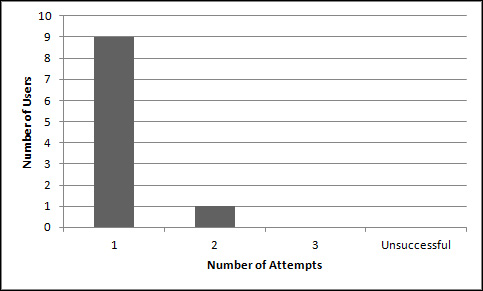
\includegraphics[width=0.9\textwidth]{ch5/Interview/EvaluationResult/PerformLogin.jpg}
\end{subfigure}%
\begin{subfigure}[b]{.5\textwidth}
  \centering
  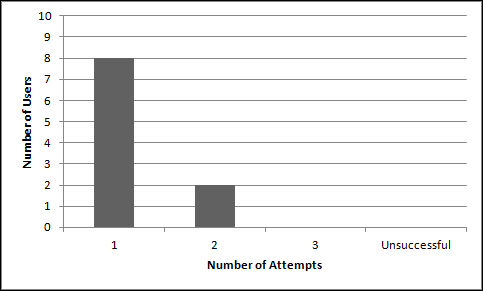
\includegraphics[width=0.9\linewidth]{ch5/Interview/EvaluationResult/SearchFoodMenu.jpg}
\end{subfigure}
\caption{Perform Login(Left).Search Food Menu(Right).}
\label{fig:EvaluationResult1}
\end{figure}

It is found that nine (9) users [figure \ref{fig:EvaluationResult1}] were able
to perform login in first attempt and only one (1) user needed two attempts. And
Eight (8) users were able to Search Food Menu in the first attempt without any
error and two (2) users took two attempts. In those tasks 100\% users are
successful.

%Create Food menu and Search friend
\begin{figure}[h!t]
\centering
\begin{subfigure}[b]{.5\textwidth}
  \centering
  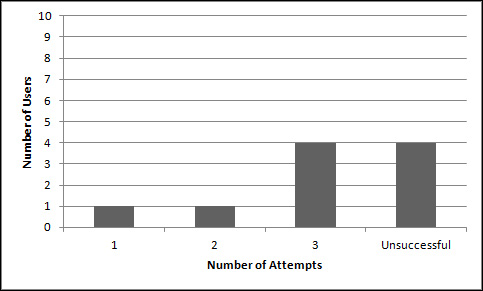
\includegraphics[width=0.9\textwidth]{ch5/Interview/EvaluationResult/CreateAFoodMenu.jpg}
\end{subfigure}%
\begin{subfigure}[b]{.5\textwidth}
  \centering
  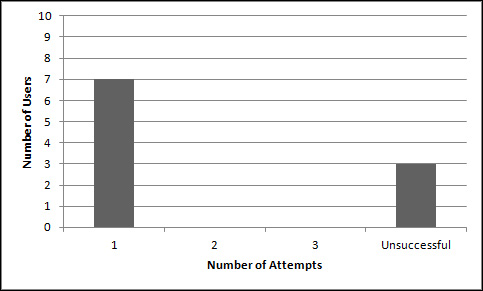
\includegraphics[width=0.9\linewidth]{ch5/Interview/EvaluationResult/SearchFriends.jpg}
\end{subfigure}
\caption{Create Food Menu(Left). Search friend(Right).}
\label{fig:EvaluationResult2}
\end{figure}

From the figure \ref{fig:EvaluationResult2}  we can see that 40\% of the users
were unsuccessfully in create food menu tasks and 30\% users were unable to
search their friends.


In the figure \ref{fig:EvaluationResult3}  shows that 60\% of the users were
able to perform these two tasks successfully in the first attempt and 100\% was
successful.
%Check your Diet Report and Check followers
\begin{figure}[h!t]
\centering
\begin{subfigure}[b]{.5\textwidth}
  \centering
  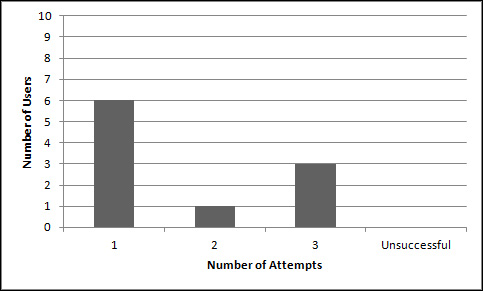
\includegraphics[width=0.9\textwidth]{ch5/Interview/EvaluationResult/CheckYourDietReport.jpg}
\end{subfigure}%
\begin{subfigure}[b]{.5\textwidth}
  \centering
  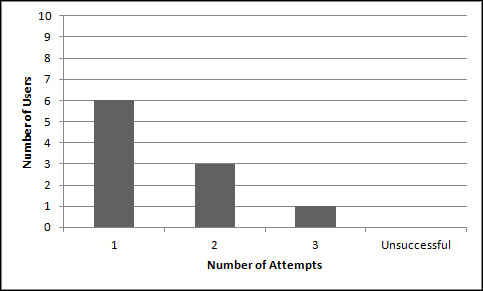
\includegraphics[width=0.9\linewidth]{ch5/Interview/EvaluationResult/CheckFollowers.jpg}
\end{subfigure}
\caption{Check your Diet Report(Left). Check followers(Right).}
\label{fig:EvaluationResult3}
\end{figure}

In case of checking time schedule [figure \ref{fig:EvaluationResult4}] and ``who
are following you'' [figure \ref{fig:EvaluationResult4}], 80\% and 70\% users
were able to perform the tasks successfully with only one attempt respectively.
%Check Time Schedule and Check who are Following you 
\begin{figure}[h!t]
\centering
\begin{subfigure}[b]{.5\textwidth}
  \centering
  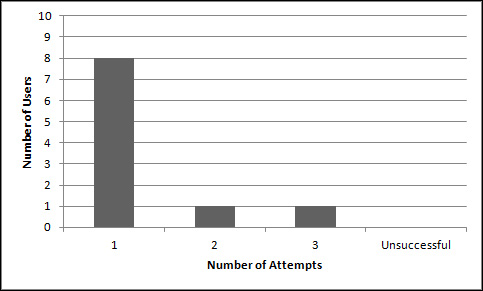
\includegraphics[width=0.9\textwidth]{ch5/Interview/EvaluationResult/CheckTimeSchedule.jpg}
\end{subfigure}%
\begin{subfigure}[b]{.5\textwidth}
  \centering
  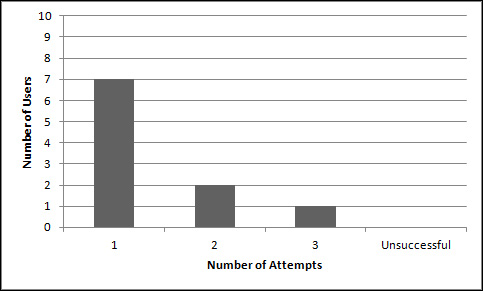
\includegraphics[width=0.9\linewidth]{ch5/Interview/EvaluationResult/CheckwhoareFollowingyou.jpg}
\end{subfigure}
\caption{Check Time Schedule(Left). Check who are Following you (Right).}
\label{fig:EvaluationResult4}
\end{figure}
\newpage
From the figure [\ref{fig:EvaluationResult5}] we can see that 90\% of the
users successfully done the task to check friend's activities successfully in
the first attempt.
%Check friend's activities
\begin{figure}[h!t]
\centering
\begin{subfigure}[b]{.5\textwidth}
  \centering
  \includegraphics[width=0.9\textwidth]{ch5/Interview/EvaluationResult/CheckFriend'sActivities.jpg}
\end{subfigure}%

\caption{Check friend's activities}
\label{fig:EvaluationResult5}
\end{figure}
 
 In the figure [\ref{ComparisonofTasksPerformance}], we can see the
 comparison of the tasks performance of the users where create food menu and
 search friends only had 40\% and 30\% unsuccessful rate, otherwise the other
 task had satisfactory performance rate.

% Comparison�of�Task Performance
\begin{figure}[h!t]
    \centering
      \includegraphics[width=5.5in,,height=3.5in]{ch5/Interview/EvaluationResult/ComparisonofTaskPerformance.jpg}
  \caption{Comparison of Tasks Performance.}
  \label{ComparisonofTasksPerformance}
\end{figure}

\subsection{Desktop Prototype Evaluation}
\label{subsec:QuestionnaireDesktop}
The study of the collected responses from the users through the questionnaire
has been presented in the tables bellow. In the
appendix[\ref{chap:UsabilityQuestionnaire}], questionnaire to measure usability
created in accordance with the USE questionnaire are provided
\cite{usabiltyUSE}. There was two part of questionnaire; firstly the general
information about the users and last part was for usability testing. The scale
of the questionnaire was based upon the Likert scale agreement or disagreement
within 7 point scale. The scale is as follows:

\begin{table}[h!t]
\centering
%\captionof{table}{Satisfaction} \label{tab:Satisfaction} 
 \begin{tabular}{| p{10cm} | p{2cm} |}
    \hline
      Likert Scale & Point  \\ \hline
      Strongly disagree & 1  \\ \hline
      Disagree & 2  \\ \hline
      More disagree than agree & 3  \\ \hline
      Neutral & 4  \\ \hline
      More agree than disagree & 5  \\ \hline
      Agree & 6  \\ \hline
      Strongly agree  & 7  \\ \hline   
    \end{tabular}
 \caption{Likert scale for Evaluation.}
\label{tab:Likertscale}
\end{table}

Ten users participated in the evaluation session. They have answered
14 usability questions which were labeled as Q1, Q2,\ldots and so on. Finally the
result was analyzed calculating Mean($\mu$) and Standard deviation($\sigma$).


Standard Deviation, $\sigma$ =  $\sqrt{\frac{1}{N}\sum_{i}^{N} (x_i - \mu^2)} $
where Mean, $\mu$ = $\frac{1}{N}\sum_{i}^{N} x_i$.

The reason of using Standard Deviation is to measure how spread feedback score
from Mean. Mean measures usability acceptance value; namely it belongs to below
neutral(scale 4)[not accepted] or upper regions from neutral(scale
4)[accepted][figure \ref{fig:EvaluationStatistics:Desktop}].


\subsubsection{Usefulness}
\label{subsub:Usefulness:Desktop}
In the first section of the questionnaire it was requested to the users for
providing their valuable feedback about the usefulness of smart cafeteria to
improve the system design.

\begin{table}[h!t]
\centering
%\captionof{table}{Usefulness} \label{tab:Usefulness} 
 \begin{tabular}{| p{6.2cm} | p{2cm} |p{4.3cm} | }
    \hline
    Questions & Mean ($\mu$) & Standard Deviation ($\sigma$) \\ \hline
    Q1. The smart cafeteria will help me to schedule my meal easily. & 4.9 & 1.663329993  \\ \hline
    Q2. This system will make my life more comfortable. & 4.3 & 1.766981104   \\   \hline
    Q3. This system will give me more control over the activities of my life. & 3.8 & 1.686548085 \\ \hline
    Q4. This system does everything I would expect it to do. & 4.3 & 1.636391694  \\   \hline
    \end{tabular}
 \caption{Usefulness[Desktop Prototype].}
\label{tab:Usefulness:Desktop}
\end{table}

From users' feedback result sheet [Appendix
\ref{sec:ResultforDesktopPrototype}], Usefulness of desktop prototype has been
calculated [Table \ref{tab:Usefulness:Desktop}]. The result sheet has shown that
``Smart Cafeteria'' system makes life easy at university and most of the users
agreed with usefulness of the new system. A significant number of users agreed
that by using this system they could find out their lunch menu easily. Half of
the user agreed that the system could make life comfortable and give more
control over activities of life; specially time at university.

\subsubsection{Ease of Use}
\label{subsub:EaseofUse:Desktop}
In second section of questionnaire, the feedback about ease of use of the ``Smart
Cafeteria'' was provided.

\begin{table}[h!t]
\centering
%\captionof{table}{Ease of Use} \label{tab:EaseofUse} 
 \begin{tabular}{| p{6.2cm} | p{2cm} |p{4.3cm} | }
    \hline
    Questions & Mean ($\mu$) & Standard Deviation ($\sigma$) \\ \hline
    Q5. The system is easy to use. & 4.9 & 1.33749351  \\ \hline
    Q6. The system requires fewest steps to accomplish what I want to do with it. & 5.1 & 1.370320319 \\ \hline
    Q7. I can use it without any written instruction. & 4.4 & 1.95505044 \\ \hline
    Q8. The system is user friendly. & 5.4 &  1.429840706 \\  \hline
    \end{tabular}
 \caption{Ease of Use [Desktop Prototype].}
\label{tab:EaseofUse:Desktop}
\end{table}

Table ``Ease of Use [Desktop Prototype]" [\ref{tab:EaseofUse:Desktop}] has been
generated from users' feedback result sheet for evaluating desktop prototype of
``Smart Cafeteria'' [Appendix \ref{sec:ResultforDesktopPrototype}]. The feedback
result has indicated that most users feel the software is easy to use and user
friendly but they have strong suggestion to include any written or visual
instruction of how to use the system.

\subsubsection{Ease of Learning}
\label{subsub:EaseofLearning:Desktop}
In the third section of questionnaire, users were asked to provide their opinion
about the system complexity of learnability.

\begin{table}[h!t]
\centering
%\captionof{table}{Ease of Learning} \label{tab:EaseofLearning} 
 \begin{tabular}{| p{6.2cm} | p{2cm} |p{4.3cm} | }
    \hline
    Questions & Mean ($\mu$) & Standard Deviation ($\sigma$) \\ \hline
    Q9. I learned to use it quickly. & 4.9 & 1.054092553 \\ \hline
    Q10. I easily remember how to use it. & 5.4 & 1.264911064 \\ \hline
    \end{tabular}
 \caption{Ease of Learning [Desktop Prototype].}
\label{tab:EaseofLearning:Desktop}
\end{table}

Table ``Ease of Learning [Desktop Prototype]" [\ref{tab:EaseofLearning:Desktop}] has
been calculated from users' feedback result sheet to evaluate desktop
prototype [Appendix \ref{sec:ResultforDesktopPrototype}]. In the feedback, more
than half of the users agreed that the desktop prototype is ease to learn.

\subsubsection{Satisfaction}
\label{subsub:Satisfaction:Desktop}
In the forth section of the questionnaire, users were asked to provide their
feedback about level of satisfaction after using the system.

\begin{table}[h!t]
\centering
%\captionof{table}{Satisfaction} \label{tab:Satisfaction} 
 \begin{tabular}{| p{6.2cm} | p{2cm} |p{4.3cm} | }
    \hline
    Questions & Mean ($\mu$) & Standard Deviation ($\sigma$) \\ \hline
    Q11. I am satisfied with it. & 4.9 & 1.888562063 \\ \hline
    Q12. It is fun to use. & 4.4 & 1.429840706 \\ \hline
    Q13. I feel I have to need it. & 4.9 & 1.286683938  \\ \hline
    Q14. I would recommend this to my friend. & 5.8 & 1.398411798 \\ \hline
    \end{tabular}
 \caption{Satisfaction [Desktop Prototype].}
\label{tab:Satisfaction:Desktop}
\end{table}

The table ``Satisfaction [Desktop Prototype]" [\ref{tab:Satisfaction:Desktop}]
has been deduced from users' feedback result sheet to evaluate desktop prototype
[Appendix \ref{sec:ResultforDesktopPrototype}]. The result sheet has shown that
more than half of the users were satisfied with the system and recommended the
system to their friends. Besides, to make the system more fun and enjoyable, it
needs more research to find out how we could make the system more fun and
attractable.

\subsubsection{Evaluation Statistics}
\label{subsub:EvaluationStatistics:Desktop}
The figure \ref{fig:EvaluationStatistics:Desktop} has shown that Q1, Q2 and Q4
feedback scores are more than neutral(scale 4) which deduces that Smart
cafeteria is usefull application in univesity. The feedback scores of questions
Q5, Q6, Q7 and Q8 are more than neutral(scale 4) which has proved that the
desktop prototype [\ref{subsec:prototypefordesktop}] of the application is easy
to use. The mean value of Q9, Q10 are more than neutral(scale 4) which ensured
that the desktop prototype [\ref{subsec:prototypefordesktop}] of the application
is easy to learn. The mean value of Q11, Q12, Q13 and Q14 are more than
neutral(scale 4) which make sure users' satisfaction when they use the system in
desktop's browser.

\begin{figure}[h!t]
    \centering
      \includegraphics[width=5.5in,,height=3.5in]{ch5/Interview/EvaluationResult/UsabilityEvaluationGraphDesktop.jpg}
  \caption{Desktop Evaluation Statistics.}
  \label{fig:EvaluationStatistics:Desktop}
\end{figure}

\newpage

\subsection{Mobile Prototype Evaluation}
\label{subsec:QuestionnaireMobile}
Mobile prototype usability evaluation has followed similar procedure as desktop
prototype evaluation [\ref{subsec:QuestionnaireDesktop}]; same amount of
users(10) have participated and same questionnaire was provided. The same
techniques has been followed or analyzing the result
[\ref{subsub:EvaluationStatistics:Mobile}]. In the following section I have
analyzed the result of mobile prototype usability evaluation [Appendix
\ref{sec:ResultforMobilePrototype}].

\subsubsection{Usefulness}
\label{subsub:Usefulness:Mobile}
\begin{table}[h!t]
\centering
%\captionof{table}{Usefulness} \label{tab:Usefulness} 
 \begin{tabular}{| p{6.2cm} | p{2cm} |p{4.3cm} | }
    \hline
    Questions & Mean ($\mu$) & Standard Deviation ($\sigma$) \\ \hline
    Q1. The smart cafeteria will help me to schedule my meal easily. & 5.9 & 1.100504935 \\ \hline
    Q2. This system will make my life more comfortable. & 5.5 & 1.178511302  \\   \hline
    Q3. This system will give me more control over the activities of my life. & 4.6 & 1.577621275 \\ \hline
    Q4. This system does everything I would expect it to do. & 5.4 & 0.966091783  \\   \hline
    \end{tabular}
 \caption{Usefulness of Smart cafeteria.}
\label{tab:Usefulness:Mobile}
\end{table}

Table \ref{tab:Usefulness:Mobile} has concluded that ``Smart Cafeteria'' will be
more usefull; specially when it will be accessible through mobile. Above 70\%
users agreed to the usefullness of ``Smart Cafeteria'' mobile application [Appendix
\ref{sec:ResultforMobilePrototype}].

\subsubsection{Ease of Use}
\label{subsub:EaseofUse:Mobile}
\begin{table}[h!t]
\centering
%\captionof{table}{Ease of Use} \label{tab:EaseofUse} 
 \begin{tabular}{| p{6.2cm} | p{2cm} |p{4.3cm} | }
    \hline
    Questions & Mean ($\mu$) & Standard Deviation ($\sigma$) \\ \hline
    Q5. The system is easy to use. & 6.1 & 0.737864787  \\ \hline
    Q6. The system requires fewest steps to accomplish what I want to do with it. & 6 & 0.816496581 \\ \hline
    Q7. I can use it without any written instruction. & 5.8 & 1.135292424 \\ \hline
    Q8. The system is user friendly. & 5.6 &  0.966091783 \\  \hline
    \end{tabular}
 \caption{Ease of Use of Smart cafeteria.}
\label{tab:EaseofUse:Mobile}
\end{table}

Table \ref{tab:EaseofUse:Mobile} has drawn a conclusion that mobile ``Smart
Cafeteria'' is easy to use. Above 80\% of users agreed with the fact that it is
easy to use [Appendix \ref{sec:ResultforMobilePrototype}].

\subsubsection{Ease of Learning}
\label{subsub:EaseofLearning:Mobile}
\begin{table}[h!t]
\centering
%\captionof{table}{Ease of Learning} \label{tab:EaseofLearning} 
 \begin{tabular}{| p{6.2cm} | p{2cm} |p{4.3cm} | }
    \hline
    Questions & Mean ($\mu$) & Standard Deviation ($\sigma$) \\ \hline
    Q9. I learned to use it quickly. & 6 & 1.054092553 \\ \hline
    Q10. I easily remember how to use it. & 6.1 & 0.567646212 \\ \hline
    \end{tabular}
 \caption{Ease of Learning of Smart cafeteria.}
\label{tab:EaseofLearning:Mobile}
\end{table}
Table \ref{tab:EaseofLearning:Mobile} has concluded that users were agreed that
the mobile application is ease to learn.

\subsubsection{Satisfaction}
\label{subsub:Satisfaction:Mobile}
\begin{table}[h!t]
\centering
%\captionof{table}{Satisfaction} \label{tab:Satisfaction} 
 \begin{tabular}{| p{6.2cm} | p{2cm} |p{4.3cm} | }
    \hline
    Questions & Mean ($\mu$) & Standard Deviation ($\sigma$) \\ \hline
    Q11. I am satisfied with it. & 5.2 & 1.135292424 \\ \hline
    Q12. It is fun to use. & 4.6 & 1.429840706 \\ \hline
    Q13. I feel I have to need it. & 5.3 & 1.766981104  \\ \hline
    Q14. I would recommend this to my friend. & 5.8 & 1.475729575 \\ \hline
    \end{tabular}
 \caption{Satisfaction of Smart cafeteria.}
\label{tab:Satisfaction:Mobile}
\end{table}
The table \ref{tab:Satisfaction:Mobile} has deduced the average satisfactory
level which are more than neutral opinion of using ``Smart Cafeteria'' mobile
application.

\subsubsection{Evaluation Statistics}
\label{subsub:EvaluationStatistics:Mobile}
The figure \ref{fig:EvaluationStatistics:Mobile} has shown that Q1, Q2, Q3 and
Q4 feedback scores are more than scale 5 which deduces that ``Smart Cafeteria"
mobile application is usefull. The feedback scores of questions Q5, Q6, Q7 and
Q8 are more than scale 5 which has proved that the mobile
prototype[\ref{subsec:PrototypeforMobile}] of the application is easy to use.
The mean value of Q9, Q10 are more than scale 5 which ensured that the mobile
prototype[\ref{subsec:PrototypeforMobile}] is easy to learn. The mean value of
Q11, Q12, Q13 and Q14 are more than neutral(scale 4) which make sure users'
satisfaction when they use ``Smart Cafeteria" in mobile.

\begin{figure}[h!t]
    \centering
      \includegraphics[width=5.5in,,height=3.5in]{ch5/Interview/EvaluationResult/UsabilityEvaluationGraphMobile.jpg}
  \caption{Mobile Evaluation Statistics.}
  \label{fig:EvaluationStatistics:Mobile}
\end{figure}


\section{Suggestions for Improvement}
The last three questions were open question to users about their suggestions,
comments about the system and which part they like most. Finally analysis of the
qualitative data we have found the following facts.

\begin{itemize}
  \item Users mostly liked parts in the system are they could know about the
  updates of food menu everyday, time schedule of cafeteria, serve menu on time
  means no queue time, dieting suggestion e.g. suggest food menu, dieting report
  e.g. calorie consumptions per month. Users also like adaptability of the
  system which is responsible for generating automatic menu suggestions and create
  customized menu functionality. Users like social collaboration activities such
  as food menu's pictures, url and real time odrer activity with friends.
  \item This part is open suggestions and comments from users. They want to see the
  following things:
  \begin{itemize}
    \item Help instruction should be provided using short video.
    \item Advanced customized food menu booking system and that should be
    clearly define with drag and drop action.
    \item Provide waiting time notification after booking the lunch. Time of
    delivery can be included with time flexibilities (In case of emergency user
    can postponed the delivery time).
    \item Inviting friends from other social media or let them know about this
    application.
    \item Brief summary of monthly calorie consumption in front page.
    \item Want to know which cafeteria is less crowded at lunch time.
    \item Should indicate which food menus are Halal(for Muslim people).
    \item Should clarify that different prices for different stakeholder;
    e.g.  Students will pay at discount rate.
    \item Should have users flexibility in cancel order or delay order option.
   \end{itemize}
\end{itemize}
Since this was the first time evaluation and user study, UI navigation and
control should be improved such that user will not face difficulties and could
understand what's going on in the system. It should include all the new
requirements of the system and conducted more survey and evaluation.


\clearpage
\newpage
%\thispagestyle{empty}
\mbox{}

\chapter{Conclusion}
\label{chap:Conclusion}
In this thesis, it has been proposed an adaptive and interactive mobile
application for Smart cafeteria which gives very essential services to students
at everyday life in university. The main objectives were (I) Create ``Smart
Cafeteria'' which will be supported by web 2.0 systems and Smartphone
application. (II) The application should be adaptive and interactive. These
objectives has been achieved by finding stakeholders, functional requirements;
developing desktop, mobile prototype and usability evaluation using HCI
interaction design methodology for ``Smart Cafeteria''.


In depth, there was some sub goals of ``Smart Cafeteria'' which overlapped with
the main objectives and those were (i) Provide online cafeteria services, (ii)
Provide dieting services to the students, and (iii) Provide social collaboration
services into the system application. To achieve those objectives and sub goals,
I have analyzed requirements, developed prototypes for desktop and mobile
related to proposed services (i) Mensa Queue Skipper, (ii) Menu Finder, (iii)
Menu Suggester and Dieting Adviser, (iv) Create Customized Menu and (v) Lunch
with Friend.


The online cafeteria services are able to skip long queue in the cafeteria and
users' are able to browse, choose and order meal in advance before entering
cafeteria. In addition, users also able to know time schedule of cafeteria using
this application. Dieting services provides some functionalities such as
generate dieting report for users, suggesting food menu based on users choice
and having calories everyday at cafeteria, generates offers and notification
through email and sms which will help student keep happy and healthy life. In
the social collaboration, users shares meal activities, status with friends.


In this thesis, ``Smart Cafeteria'' has been analyzed, proposed the application,
designed both UI prototype for desktop and mobile, and finally usability
evaluation has been performed by through users' study. From the users'
evaluation, it is proven that it is essential providing quality services in
cafeteria for achieving the goal of a smart campus. By this proposed cafeteria
application's ideas and functionalities, the goals of ``Smart Cafeteria'' have
been achieved.


\section{Further Work}
\label{sec:FurtherWork}
Since this is the first time analysis and designs such an application in
cafeteria domain to provide services through mobile as well as browser to the
university students, it is very important to design high fidelity prototype,
programming model such as ORM model, controller, view and service oriented
architecture (SOA) to provide real services to users.


This moment, I have developed UML model and UI of application to demonstrate
``Smart Cafeteria'' and evaluated user experience following interactive design
methodology.  In future I will extend the work and build high fidelity
prototype, develop mobile services and perform users study to evaluate the
system again until maximum level of usability. I will do also more work with
application's adaptation using various machines learning approaches and figure
out which will be the best for ``Smart Cafeteria''. Finally I will develop rest of
the parts as full functional application of ``Smart Cafeteria'' which will ensure
more interactive, adaptability and usability.



%for bib file
\bibliographystyle{IEEEtranN}% ieeetr,plain,acm,unsrtnat
\cleardoublepage
\phantomsection
\addcontentsline{toc}{chapter}{References}
%\addcontentsline{toc}{chapter}{Bibliography}
\bibliography{SmartCafeteriabib}% .bib tex file

%for normal 99 references stype
%\input{bibliography.tex}

\begin{appendices}
\chapter{Data and Requirements Gathering}
\section{Studying Documents and Research}
\label{sec:MenuAppendix}
\begin{figure}[h!t]
    \centering
      \includegraphics[width=5.5in,height=2in]{ch3/AppendixMenu/differentmenu}
  \caption{different menu of Mensa in University of Trento.}
  \label{differentmenu}
\end{figure}
\newpage \begin{figure}[h!t]
    \centering
      \includegraphics[width=5.5in,height=4in]{ch3/AppendixMenu/timeschedule}
  \caption{Time Schedule of Mensa in University of Trento.}
  \label{timeschedule}
\end{figure}
\newpage \begin{figure}[h!t]
    \centering
      \includegraphics[width=5.5in,height=4in]{ch3/AppendixMenu/Weeklylunchmenu}
  \caption{Weekly lunch menu of Mensa in University of Trento.}
  \label{Weeklylunchmenu}
\end{figure}
\newpage
\section{Focus Group and Workshop}
\label{sec:AppendixFocusGroup}
\begin{figure}[h!t]
    \centering
      \includegraphics[width=5.5in]{ch3/AppendixFocusGroup/FocusGroup}
  \caption{FocusGroup}
  \label{FocusGroup}
\end{figure}
\newpage

\section{Data Gathering Questionnaire \& Result}
\label{sec:DataGatheringQuestionnaire}
\begin{figure}[h!t]
    \centering
      \includegraphics[width=5.5in]{ch3/AppendixQuestionnaires/Questionnaire}
  \caption{Questionnaire}
  \label{Questionnaire}
\end{figure}

\chapter{Usability Evaluation}
\label{chap:UsabilityQuestionnaire}
\section{Usability Evaluation Questionnaire}
\label{sec:UsabilityEvaluationQuestionnaire}
%\includepdf[pages={1,2,3,4},scale=.8]{ch5/QuestionnaireSmartCafeteria.pdf}

\begin{figure}[h!t]
    \centering
      \includegraphics[height=4.7in, width=6in]{ch5/UsabilityQuestionnaire1.pdf}
  %\caption{Usability Questionnaire}
  \label{UsabilityQuestionnaire1}
  
\end{figure}


\begin{figure}[h!t]
    \centering
      \includegraphics[width=6in]{ch5/UsabilityQuestionnaire2.pdf}
  %\caption{Usability Questionnaire}
  \label{UsabilityQuestionnaire2}
\end{figure}


\begin{figure}[h!t]
    \centering
      \includegraphics[width=6in]{ch5/UsabilityQuestionnaire3.pdf}
  %\caption{Usability Questionnaire}
  \label{UsabilityQuestionnaire3}
\end{figure}


\begin{figure}[h!t]
    \centering
      \includegraphics[width=6in]{ch5/UsabilityQuestionnaire4.pdf}
  %\caption{Usability Questionnaire}
  \label{UsabilityQuestionnaire4}
\end{figure}

\clearpage
\newpage
\section{Result of Desktop Prototype Evaluation}
\label{sec:ResultforDesktopPrototype}

\begin{figure}[h!t]
    \centering
      \includegraphics[width=5.6in]{ch5/Result/Desktop/1.pdf}
  %\caption{Usability Questionnaire}
  \label{fig:Result:Usefulness:EaseofLearning:Desktop}
\end{figure}

\begin{figure}[h!t]
    \centering
      \includegraphics[width=6in]{ch5/Result/Desktop/2.pdf}
  %\caption{Usability Questionnaire}
  \label{fig:Result:EUS:Desktop}
\end{figure}


\begin{figure}[h!t]
    \centering
      \includegraphics[width=6in]{ch5/Result/Desktop/3.pdf}
  %\caption{Usability Questionnaire}
  \label{fig:Result:Analysis:Desktop}
\end{figure}

\clearpage
\newpage
\section{Result of Mobile Prototype Evaluation}
\label{sec:ResultforMobilePrototype}

\begin{figure}[h!t]
    \centering
      \includegraphics[width=5.6in]{ch5/Result/Mobile/1.pdf}
  %\caption{Usability Questionnaire}
  \label{fig:Result:Usefulness:EaseofLearning:Mobile}
\end{figure}

\begin{figure}[h!t]
    \centering
      \includegraphics[width=6in]{ch5/Result/Mobile/2.pdf}
  %\caption{Usability Questionnaire}
  \label{fig:Result:EUS:Mobile}
\end{figure}


\begin{figure}[h!t]
    \centering
      \includegraphics[width=6in]{ch5/Result/Mobile/3.pdf}
  %\caption{Usability Questionnaire}
  \label{fig:Result:Analysis:Mobile}
\end{figure}

\end{appendices}




\end{document}

